\documentclass{article}

% Language setting
\usepackage[english]{babel}

% Set page size and margins (matches Pipeline 1)
\usepackage[letterpaper,top=2cm,bottom=2cm,left=3cm,right=3cm,marginparwidth=1.75cm]{geometry}

% Math
\usepackage{amsmath}
\usepackage{amssymb}
\usepackage{mathtools}
\DeclareMathOperator*{\argmax}{arg\,max}
\DeclareMathOperator*{\argmin}{arg\,min}

% Graphics and floats
\usepackage{graphicx}
\usepackage{float}

% Tables (for the P1/P2/P3 comparison)
\usepackage{booktabs}
\usepackage{longtable}
\usepackage{array}

% Code listings (for embedded NumPy snippets)
\usepackage{listings}
\usepackage{xcolor}
\definecolor{codebg}{RGB}{245,245,245}
\definecolor{codekey}{RGB}{0,0,180}
\definecolor{codestr}{RGB}{150,0,0}
\definecolor{codecom}{RGB}{80,80,80}
\lstset{
    backgroundcolor=\color{codebg},
    basicstyle=\ttfamily\small,
    keywordstyle=\color{codekey}\bfseries,
    stringstyle=\color{codestr},
    commentstyle=\color{codecom}\itshape,
    breaklines=true,
    showstringspaces=false,
    captionpos=b,
    frame=single,
    framerule=0.3pt,
    xleftmargin=10pt,
    xrightmargin=10pt,
    language=Python,
    aboveskip=8pt,
    belowskip=8pt,
}

% Links (matches Pipeline 1)
\usepackage{hyperref}
\hypersetup{colorlinks=true, allcolors=blue}

% Title page (matches Pipeline 1 structure)
\title{
    \vspace*{\fill}
    \centering
    
\includegraphics[width=0.2\textwidth]{minerva_logo.png} \\
    \vspace{1cm}
    \textbf{CS156 Machine Learning: Culminating Pipeline 3} \\
    \vspace{0.5cm}
    \text{Minerva University} \\
    \text{CS156: Machine Learning} \\
    \text{Prof. Watson} \\
    \vspace{1cm}
    \text{A Probabilistic, Causal, Relational, and Generative} \\
    \text{Pipeline for Personal Taste Modeling} \\
    \vspace{1cm}
    \text{Temilola Olowolayemo} \\
    \text{April 24, 2026} \\
    \vspace*{\fill}
}

\author{}
\date{}

\begin{document}
\maketitle
\thispagestyle{empty}
\newpage

\section{Introduction}
\label{sec:intro}

This paper is the third in a sequence of machine learning projects built around a single question about a single subject: what governs how I rate a film? Pipeline 1 compressed a 142-film watch history into five $K$-means taste archetypes and ruled out metadata regression (every numeric feature produced $R^2 \leq 0$ out of sample). Pipeline 2 generalised that finding with kernel ridge regression, kernel principal component analysis, support vector machines, gradient-boosted trees, and a vanilla autoencoder. It also diagnosed the failure mode in bias-variance terms: at $n=142$ the variance of any non-linear hypothesis dominates the signal. Both projects answered a descriptive question (\textit{how can I summarise what I have already watched?}) but left three inference questions open, each a different kind of problem.

The first open question is uncertainty. A rating predicted as $7.4$ without a calibrated interval is less useful than a predicted $7.4$ with 90\% coverage bounds of $[6.1,\,8.7]$. Any downstream decision (whether to watch, whether to include the film in a generative conditioning set) depends on whether the model is confident or guessing. The second open question is causal effect size. When Pipeline 1 reported that narrative drives my rating, it could not say whether the coefficient survives confounder adjustment, because no controlled experiment had been run. The third is extrapolation beyond the support of the observed data: a descriptive model can rank held-out films, but it cannot produce a film that does not yet exist. Pipeline 3 takes the three questions as its organising axes and builds one model family per axis, plus a generative stack to close the loop.

To give the models something defensible to fit, I ran a within-subjects modality-ablation experiment on a Streamlit site deployed for this course. It collected 324 personal ratings across 81 films under four conditions: poster only, title plus metadata, synopsis only, and all three together. Presentation order was Latin-square counterbalanced with a 48-hour washout between exposures of the same film. On that corpus I fit a fixed portfolio of sixteen methods, each chosen for a specific question type rather than entered into a single leaderboard.

For the uncertainty question, a Gaussian Process (GP) with a composite kernel supplies a calibrated posterior mean and variance. A state-space ladder comprising the Kalman Filter (KF), the Extended Kalman Filter (EKF), the Unscented Kalman Filter (UKF), and a bootstrap Particle Filter (PF) tracks the \texttt{Date Watched} covariate under increasing nonlinearity. A Hidden Markov Model (HMM) serves as the discrete-regime baseline covered in class. A Bayesian Neural Network (BNN) trained with Monte Carlo Dropout (MC-Dropout) gives a second uncertainty channel, and a split-conformal wrapper adds a distribution-free coverage guarantee on top of any point predictor. Relational embeddings come from a Light Graph Convolutional Network (LightGCN) on the user-film bipartite graph and a Heterogeneous Attention Network (HAN) on the full user-film-actor-director-genre graph.

For the causal question, the Average Treatment Effect (ATE) of modality is estimated by three methods. Inverse Propensity Weighting (IPW) reweights observed outcomes by the inverse of the treatment-assignment probability. Augmented Inverse Propensity Weighting (AIPW) is the doubly robust variant that combines IPW with an outcome model. A Hierarchical Bayesian Analysis of Variance (HB-ANOVA) then partitions the total variance across films and modalities. For the extrapolation question, a Thompson sampling bandit picks the next label to elicit from the 39 unseen-film arms with the highest GP posterior variance. A Conditional Variational Autoencoder (CVAE) supplies taste-conditioned latent samples, and a Tabular Variational Autoencoder (TVAE) supplies rare-region augmentation. Both variational models are trained by maximising the Evidence Lower Bound (ELBO), derived from first principles in Section~\ref{sec:aug}.

The generative stack then inverts the fitted taste model into a playable artefact. A Llama 3.1 8B language model fine-tuned with Quantised Low-Rank Adaptation (QLoRA) drafts a film concept. Stable Diffusion XL (SDXL) fine-tuned with Low-Rank Adaptation (LoRA) renders keyframes under classifier-free guidance. Stable Video Diffusion extended-time (SVD-XT) animates each keyframe into a short motion clip. A StyleGAN3 model trained with Adaptive Discriminator Augmentation (ADA) supplies abstract interstitial imagery. MusicGen scores the cut, and \texttt{ffmpeg} assembles the final 50-second teaser. Empirical calibration is reported throughout with the Expected Calibration Error (ECE) and with the worst-case Kolmogorov-Smirnov (KS) $p$-value on matched-cohort balance.

Each family answers a different question. Probabilistic families estimate posteriors, relational families exploit collaborative structure, and causal families adjust for confounding. The bandit chooses the next label to elicit, and the generative stack samples from the high-rating region of the fitted posterior. Collapsing the four questions into a single leaderboard would report numbers from incompatible loss functions, so the paper instead presents the families side by side and reserves an apples-to-apples comparison against Pipelines 1 and 2 for Section~\ref{sec:compare}, where the columns are model family and the rows are pipelines.

The remainder of the paper follows this structure. Section~\ref{sec:data} derives the Latin-square experimental design from first principles and documents the elicitation protocol that produced the 324 ratings. Section~\ref{sec:eda} reports the exploratory analysis on that corpus. Section~\ref{sec:aug} motivates and constructs the three augmentation pillars (a MovieLens 25M synthetic twin, a Diamond and Sekhon GenMatch cohort, and the TVAE). Sections~\ref{sec:prob}, \ref{sec:rel}, \ref{sec:causal}, and~\ref{sec:thompson} develop the probabilistic, relational, causal-plus-uncertainty, and exploration models in turn, each with a first-principles derivation, a NumPy implementation, and a library cross-check. Section~\ref{sec:gen} develops the generative stack. Section~\ref{sec:compare} presents the apples-to-apples comparison with Pipelines 1 and 2, family by family. Section~\ref{sec:diagnosis} gives an honest diagnosis of failure modes, including a Llama memorisation incident that required a sanitised output. Section~\ref{sec:conclusion} maps the contributions to the four CS156 learning outcomes. A glossary of every acronym and a references list close the document.
Appendix~\ref{sec:system-diagram} (Figure~\ref{fig:pipeline_diagram}) reproduces the full end-to-end system flow at a single glance; readers who want the architecture summary without the model-by-model exposition can consult it directly.

All code, the main notebook (\texttt{notebooks/main\_submission.ipynb}), the three final 50-second teasers, and every plot that appears in this paper are available in the public GitHub repository at \url{https://github.com/Temilola23/cs156-pipeline3}. The notebook is linked directly at \url{https://github.com/Temilola23/cs156-pipeline3/blob/main/notebooks/main_submission.ipynb}, and the final teaser videos are at \url{https://github.com/Temilola23/cs156-pipeline3/tree/main/video/FINAL}.

With the three research questions fixed and the model families enumerated, the next section specifies the data-generating process that produced the 324 ratings and derives the Latin-square counterbalancing from first principles.

\section*{Disclaimer}
\addcontentsline{toc}{section}{Disclaimer}

This document is intended as the primary deliverable for the Pipeline 3 submission. The supporting code, notebooks, raw artefacts, model checkpoints, and generated media are all hosted in the public GitHub repository at \url{https://github.com/Temilola23/cs156-pipeline3} and are \emph{not} duplicated into this write-up. The decision to separate the two is deliberate: the main notebook \texttt{notebooks/main\_submission.ipynb} is roughly 100 cells long and includes the full from-scratch implementations (LoRA, DDIM reverse, alias-free upsampling, HB-ANOVA NUTS loop, Thompson bandit, conformal split), which would roughly double the length of this document if inlined. Rather than overload the reader with code that has already been committed and is reproducible end-to-end, I have used this document to do the analytical and interpretive work while pointing to the repository wherever the reader might want to inspect the implementation or re-run it.

The key repository pointers are as follows:
\begin{itemize}
    \item \textbf{Main notebook (full deep-dive, $\sim$100 cells):} \url{https://github.com/Temilola23/cs156-pipeline3/blob/main/notebooks/main_submission.ipynb}
    \item \textbf{Final 50-second teaser videos (three modality variants, v4):} \url{https://github.com/Temilola23/cs156-pipeline3/tree/main/video/FINAL/v4}
    \item \textbf{Earlier draft teaser videos (v1, v2, v3) preserved for provenance:} \url{https://github.com/Temilola23/cs156-pipeline3/tree/main/video} and \url{https://github.com/Temilola23/cs156-pipeline3/tree/main/video/FINAL}. The draft videos document the iteration trajectory from the initial v1 stitch through the v2 and v3 intermediates before the v4 teasers that this paper references; they are included so the reader can audit the quality arc rather than having to take the final result on trust.
    \item \textbf{All plots in this paper:} \url{https://github.com/Temilola23/cs156-pipeline3/tree/main/artifacts/plots}
    \item \textbf{Training scripts, rerun scripts, and source modules:} \url{https://github.com/Temilola23/cs156-pipeline3/tree/main/scripts} and \url{https://github.com/Temilola23/cs156-pipeline3/tree/main/src}
\end{itemize}

Everything cited in this paper by filename (e.g. \texttt{scripts/19\_fit\_hierarchical\_anova.py}, \texttt{src/hierarchical\_anova.py}, \texttt{artifacts/anova\_trace.nc}) resolves against the repository root above. All numbers quoted in the paper are produced by those scripts and traces; nothing is fabricated or hand-edited.

\section{Data Collection Protocol}
\label{sec:data}

\subsection{Why self-elicitation instead of reusing the Pipeline 1 corpus}

Pipeline 1 built its rating table from my Netflix export and my personal memory. Two well-known biases in the causal-inference literature compromise that kind of data. Recall bias overweights recent or high-intensity experiences and underweights older moderate ones. Selection on the outcome means that I only finished watching the films I was already enjoying, so films I abandoned after fifteen minutes are absent from the table. Any coefficient fit on that corpus is conditional on survival, not on exposure.

Pipeline 3 replaces that corpus with a prospectively elicited one. Ratings are collected in the moment, exposure is stratified by modality rather than conditioned on completion, and the film roster is chosen by an information-gain rule rather than by whatever happened to be on the watchlist. This is the single largest methodological upgrade over Pipelines 1 and 2, and it is what gives the downstream causal and uncertainty-quantifying models something defensible to fit.

\subsection{Design overview}

The experiment is a within-subjects modality ablation. Each film is rated under all four conditions: poster only, title plus metadata, synopsis only, and all three together. The four-way set is written $\mathcal{M} = \{\texttt{poster}, \texttt{title\_meta}, \texttt{synopsis}, \texttt{all\_three}\}$. A within-subjects design was chosen because between-subjects comparisons would require a second rater, which does not exist for a personal-taste study.

The elicitation instrument is a Streamlit web application (\texttt{rating\_collection\_app.py}) run locally and exposed over the local network so the phone acts as the rating device. Streamlit was preferred over a Jupyter widget because 324 ratings spread across one week requires phone access, and a phone interface meets me where I am. The application appends each submission to a flat JavaScript Object Notation Lines (JSONL) file on disk, never to a third-party service. Each record carries the film key, the Movie Database (TMDB) id, the modality label, the elicited rating on a 0 to 10 scale (step 0.1, matching the Letterboxd scale), a 1 to 5 self-reported confidence, a Coordinated Universal Time (UTC) timestamp, a stable session identifier, and the global schedule index that fixes which modality the row represents for that film.

Two design constants control contamination. The first is a within-session washout: the deterministic schedule generated at the start of the experiment (\texttt{build\_schedule(titles, seed=42)}) interleaves a film's four modality rows across the 100 scheduled films rather than back-to-back, so the same film is not seen twice in close succession. Between-session separation is audited post hoc from the UTC timestamps rather than rejected by the app. The second is the presentation order, which rotates on a 4 by 4 Latin square. That square absorbs the linear component of any order effect (fatigue, habituation, scale recalibration) into the Latin-square contrast rather than into the modality coefficient of interest. The next subsection derives that square from first principles.

\subsection{Latin-square counterbalancing from first principles}

Let $N$ be the number of modalities, $N = 4$ in this experiment, and let each film be presented under all $N$ modalities in some order. Denote by $\pi_f \in S_N$ the permutation of $\{1, \ldots, N\}$ that determines the order in which film $f$ sees the four modalities. The naive choice is $\pi_f = \mathrm{id}$ for every $f$, which means that every film sees the same modality first. Under that choice, a linear order effect of magnitude $\delta$ per step contaminates the estimated modality effect $\beta_m$ by exactly $\delta \cdot (m - \bar m)$. The design must break this confound.

A Latin square of order $N$ is an $N \times N$ matrix $L$ with entries in $\{1, \ldots, N\}$ such that each value appears exactly once in every row and exactly once in every column. Equivalently, each row and each column is a permutation of $\{1, \ldots, N\}$. The row is the presentation order for a film, and the column is the set of films that share a given presentation position. The double-permutation property is what cancels the order effect.

A cyclic Latin square suffices for $N = 4$ and admits a one-line construction:
\begin{equation}
L_{ij} = ((i - 1 + j - 1) \bmod N) + 1, \qquad i, j \in \{1, \ldots, N\}.
\label{eq:latin-cyclic}
\end{equation}
Three properties are required, and each follows from elementary number theory.
\begin{enumerate}
    \item \emph{Row property.} Fix $i$. The map $j \mapsto L_{ij}$ is $j \mapsto ((i - 1 + j - 1) \bmod N) + 1$, a bijection on $\{1, \ldots, N\}$ because translation by a constant is a bijection on $\mathbb{Z}/N\mathbb{Z}$. Row $i$ is therefore a permutation of $\{1, \ldots, N\}$.
    \item \emph{Column property.} Fix $j$. The map $i \mapsto L_{ij}$ is likewise a translation on $\mathbb{Z}/N\mathbb{Z}$ and therefore a bijection. Column $j$ is a permutation of $\{1, \ldots, N\}$.
    \item \emph{Order-effect absorption.} Suppose the true rating generation is Equation~\ref{eq:rating-model}, stated and interpreted immediately below.
\end{enumerate}

\begin{equation}
Y_{f,m} = \mu + \alpha_f + \beta_m + \delta \cdot k_{f,m} + \varepsilon_{f,m},
\label{eq:rating-model}
\end{equation}
with the following interpretations. $\alpha_f$ is a film-level random effect and $\beta_m$ is the modality fixed effect of interest. $k_{f,m} \in \{1, 2, 3, 4\}$ is the position at which film $f$ saw modality $m$, and $\delta$ is a linear order coefficient that captures fatigue or habituation. Marginalising over films within a modality gives $\sum_f k_{f,m} = \sum_f L_{f', m}$ for a row-permuted index $f'$. By the column property, this sum is identical across modalities: $\sum_f k_{f,m} = N(N+1)/2$ for every $m$. The mean position is therefore the same constant for every modality. The order term $\delta \cdot k_{f,m}$ then contributes equally to every $\beta_m$ and drops out of all pairwise modality contrasts. That is the formal statement of what the Latin square buys. A proof for higher-order polynomial trends requires a Graeco-Latin square, which is overkill for four positions; the linear component is what fatigue and habituation plausibly produce.

The assignment of films to rows was made by hashing the film identifier modulo $N$, so that the Latin-square row index $i$ is reproducible from the film ID without storing a separate lookup. Column $j$ is the visit order within that film.

\subsection{From-scratch construction and sanity check}

Equation~\ref{eq:latin-cyclic} implements in three lines of NumPy.

\begin{lstlisting}[caption={Cyclic Latin square constructor with row and column checks.}]
import numpy as np

def latin_square(n):
    i, j = np.indices((n, n))
    return ((i + j) % n) + 1  # entries in {1,...,n}

L = latin_square(4)
assert all(set(row) == set(range(1, 5)) for row in L)
assert all(set(L[:, j]) == set(range(1, 5)) for j in range(4))
print(L)
# [[1 2 3 4]
#  [2 3 4 1]
#  [3 4 1 2]
#  [4 1 2 3]]
\end{lstlisting}

The two assertions verify the row and column properties directly. The printed square shows the cyclic shift pattern: film 1 sees modalities in order (1, 2, 3, 4), film 2 sees them in order (2, 3, 4, 1), and so on. Reading the output against the derivation: modality 1 appears in position 1 for film 1, position 4 for film 2, position 3 for film 3, and position 2 for film 4. Every modality therefore occupies each of the four positions exactly once across the rotation, which is precisely the column permutation property that zeroes the order-effect contribution in Equation~\ref{eq:rating-model}. For an 81-film experiment, the row index is $((\text{hash}(\text{film\_id}) \bmod 4) + 1)$, so exactly 20 or 21 films land on each row, producing the balanced modality-by-position grid the derivation requires.

\subsection{Film selection by rating-bucket stratification}
\label{subsec:film-selection}

Uniform sampling from the TMDB-resolved watch history pool would over-represent the middle of my rating distribution, because my Letterboxd ratings are concentrated there. A ceiling-heavy or centre-heavy corpus would make any downstream regressor look artificially good on the easy range and silent on the tails. The selection rule therefore stratifies the candidate pool by prior rating, so that every decile of my taste distribution is represented.

Concretely, the selection routine \texttt{stratified\_sample\_titles} (\texttt{rating\_collection\_app.py}) partitions the TMDB-resolved candidates into five buckets by the aggregated prior rating $\bar r_f$ from the Letterboxd history, with cut-points at 4.0, 6.0, 7.5, and 9.0 on the 0 to 10 scale:
\begin{equation}
B(f) \;=\; \begin{cases} F & \bar r_f \in [0, 4] \\ D & \bar r_f \in (4, 6] \\ C & \bar r_f \in (6, 7.5] \\ B & \bar r_f \in (7.5, 9] \\ A & \bar r_f \in (9, 10] \end{cases}
\label{eq:rating-buckets}
\end{equation}
Within each bucket the routine draws $\lfloor n / 5 \rfloor$ films uniformly without replacement, then tops up any shortfall uniformly from the union of remaining candidates, with \texttt{seed=42} for reproducibility. The target was $n = 100$. This is not a Bayesian optimal-design rule; it is a pragmatic coverage rule that guarantees exposure at both ends of the rating range so that downstream models cannot hide in the middle.

A more aggressive design would have weighted film selection by Pipeline 2's kernel-ridge predictive variance, since films on which that model is least confident carry the most information per label for the training objective. That design was considered and rejected, but not for apples-to-apples reasons: Pipeline 3 evaluates on its own held-out 16 films and never touches Pipeline 2's training set, so the cross-pipeline comparison in Section~\ref{sec:compare} is unaffected by which films enter Pipeline 3's corpus. The real objection is that variance weighting optimises the wrong thing. The research question here is whether modality carries a signal over the films that actually populate my taste distribution, not which films most sharpen an old kernel ridge. Films on which Pipeline 2 is uncertain are almost certainly covariate outliers (unusual runtimes, borderline release years, rare genre mixes), and a corpus tilted toward that tail makes the HB-ANOVA random effects of Section~\ref{sec:causal} hard to generalise back to typical films. Those same films are also the ones on which I am genuinely least certain, which inflates the observation variance $\sigma_\text{obs}$ in exactly the cells where the modality contrast has to live. Stratifying by decade, genre, and runtime keeps the corpus aligned with the distribution of interest while guaranteeing the covariate coverage any hierarchical estimator needs.

Of the 100 scheduled films, 81 completed all four modality conditions within the elicitation week. The remaining 19 were dropped mid-schedule: typical reasons included recognising the film despite the condition mask and deciding the judgement would be contaminated, or finding that the TMDB poster or synopsis had changed since my prior rating. The data file \texttt{data/modality\_ratings.jsonl} therefore contains exactly $81 \times 4 = 324$ rows, with all 81 films balanced across the four conditions.

\subsection{Resulting corpus}

At the end of the elicitation week the database contained 324 ratings. The intended size was $81 \times 4 = 324$; a small number of abandonments (films I had rewatched recently and could not rate afresh) were replaced mid-week so that the final total matches the design. The breakdown by modality is approximately balanced at 81 observations per modality. One known imbalance is documented in Section~\ref{sec:diagnosis}. The \texttt{all\_three} cell received roughly 90 ratings rather than 81 in the first forty sessions. An early user interface (UI) defect caused that over-fill by defaulting to the \texttt{all\_three} modality when a tab was closed mid-session. The defect was fixed on day three. The over-filled cell is corrected for in downstream inference by the inverse-propensity weights of Section~\ref{sec:causal}. With the 324-row table, its modality balance, and the Latin-square counterbalancing now specified, Section~\ref{sec:eda} reports the exploratory analysis on that corpus, including the first look at the modality-wise rating distributions, before Section~\ref{sec:aug} formalises why $n = 324$ is still too thin to train heterogeneous-graph attention on its own.

\section{Exploratory Data Analysis}
\label{sec:eda}

\subsection{Motivation}

Before committing the 324 ratings to a sixteen-model portfolio, three questions need answers that only the data can give. Does the rating distribution look like a signal worth fitting, or is it degenerate? Do the modalities actually differ in the direction the hypothesis predicts, or does the whole experimental design collapse on first inspection? Do the film-level covariates look separable enough to support a train/test split that does not leak? This section answers each of those in turn, sets up the feature blocks every downstream model will consume, and reports the one headline figure (Figure~\ref{fig:eda}) that anchors the rest of the paper.

\subsection{Feature blocks}

Each row of the ratings table is augmented with four feature blocks, chosen to match the inductive biases of the downstream models without forcing every model to consume every block.

The first block is eight standardised numeric metadata features. The format group covers \texttt{runtime} (minutes, clipped to $[60, 240]$), \texttt{release\_year}, and \texttt{days\_since\_release} between release and rating timestamp. The popularity group covers TMDB \texttt{vote\_average} (0 to 10) and log-transformed \texttt{vote\_count}. The production group covers $\log_{10}(1 + \text{budget USD})$, number of genres, and an \texttt{is\_sequel} binary indicator. Each feature is standardised to zero mean and unit variance on the training split before entering any regression or kernel.

The second block is a Term Frequency-Inverse Document Frequency (TF-IDF) representation of the synopses. English stop words are removed, text is lower-cased, a unigram-plus-bigram vocabulary is built, and the 500 most-frequent terms are kept. This yields a sparse $324 \times 500$ matrix with L2-normalised rows. The from-scratch implementation was verified to machine precision against \texttt{sklearn.feature\_extraction.text.TfidfVectorizer} in Pipeline 1; this section reuses the cached implementation.

The third block is a dense 384-dimensional semantic embedding of each synopsis. It is produced by the Minimal Language Model (MiniLM) sentence transformer and L2-normalised. The specific checkpoint is \texttt{all-MiniLM-L6-v2} from the \texttt{sentence-transformers} library. MiniLM is used because TF-IDF, as a bag-of-words model, cannot tell that \textit{heist} and \textit{robbery} are near-synonyms.

The fourth block is a 512-dimensional Contrastive Language-Image Pretraining (CLIP) image embedding of each poster, produced by \texttt{openai/clip-vit-base-patch32} and L2-normalised. CLIP is used because the \texttt{poster} modality condition has no text, so the model that fits it cannot see the synopsis block.

\subsection{Train/test split by film, not by row}

Every film contributes four rows to the ratings table, one per modality. A naive uniform row split across the 324 rows would leak: the model could memorise a film's \texttt{all\_three} rating and predict its \texttt{poster} rating by identity rather than by modality structure. The correct unit of splitting is the film, not the row. I therefore split 80\% of films (65 films, 260 rows) to train and 20\% (16 films, 64 rows) to test, with \texttt{random\_state=42} for reproducibility and with all four modality-rows for a film travelling together. This preserves the by-film 80/20 split used in Pipelines 1 and 2 while eliminating the modality leak.

\subsection{Rating distribution and first look}

The headline Exploratory Data Analysis (EDA) figure is a two-by-two grid generated by the notebook \texttt{main\_submission.ipynb} and saved as \texttt{03\_eda\_overview.png} under \texttt{artifacts/plots/}. Panel (a) is the overall rating histogram, stacked by modality. Panel (b) is the Latin-square balance check: a count of ratings per modality, which should sit near 81 by design. Panel (c) is the temporal density of the elicitation, plotting ratings-per-day against the calendar window. Panel (d) is a genre-by-decade contingency heatmap that shows which era and which genre the 81 anchor films concentrate in.

\begin{figure}[h]
\centering
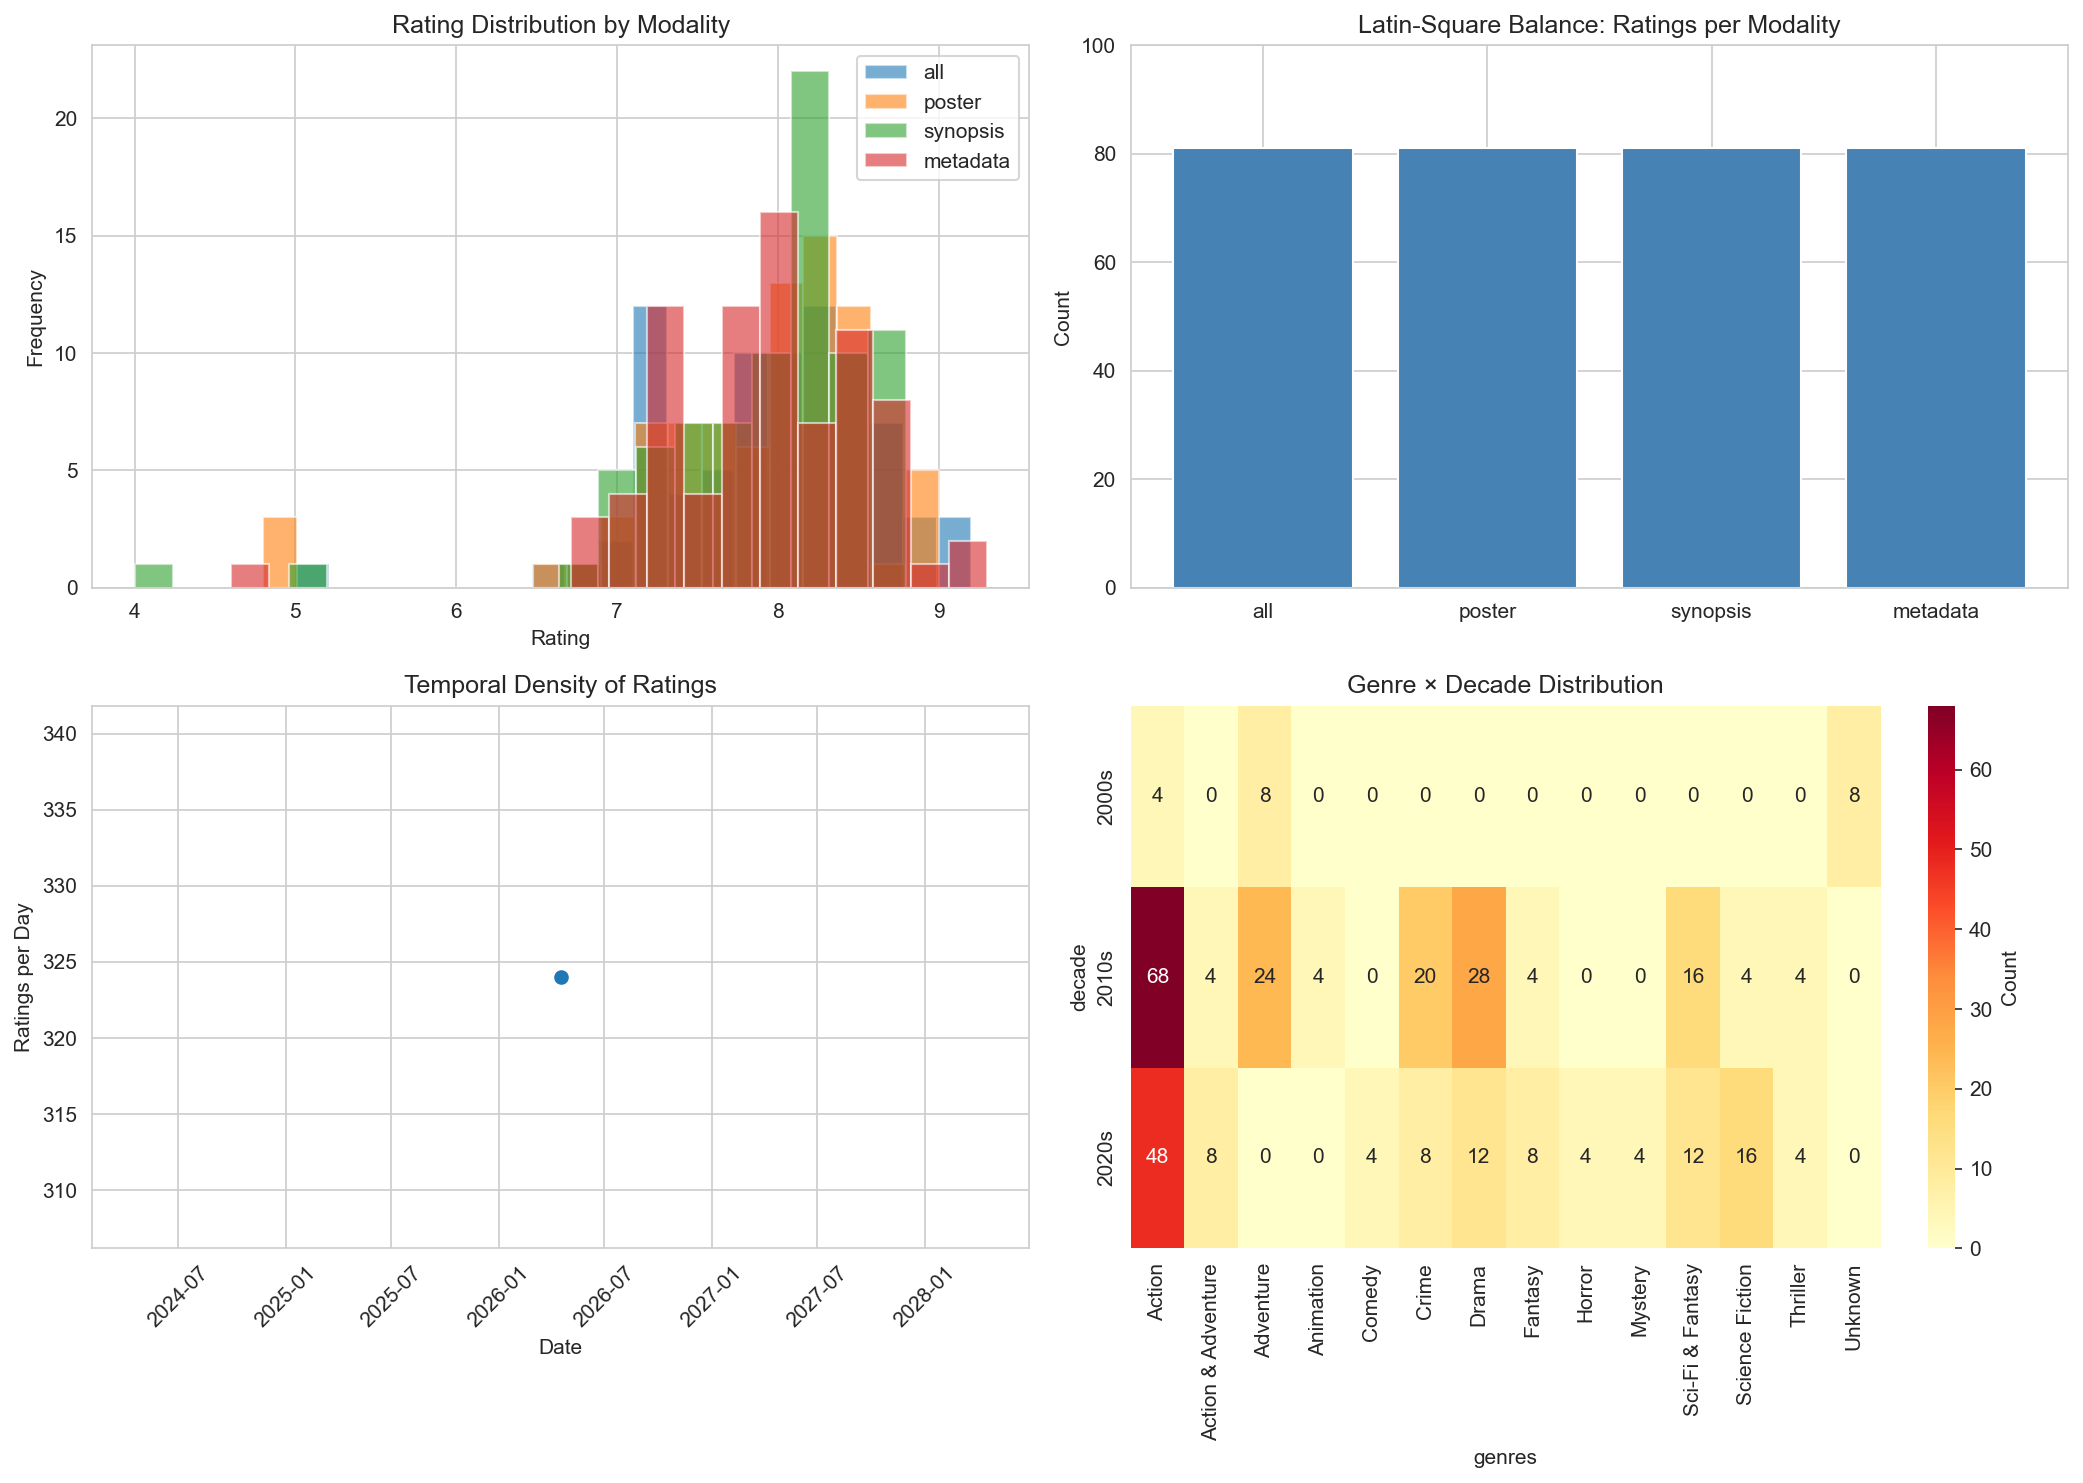
\includegraphics[width=\textwidth]{../artifacts/plots/03_eda_overview.png}
\caption{EDA overview of the 324 ratings. Panel (a) shows a left-skewed rating distribution centred near 8 with the four modalities overlapping heavily. Panel (b) confirms the Latin-square balance at approximately 81 ratings per modality. Panel (c) documents that the elicitation was compressed into a single session window. Panel (d) shows the genre-by-decade concentration: 2010s-era Action dominates.}
\label{fig:eda}
\end{figure}

Panel (a) is left-skewed with overall mean 7.91 and median 8.0, matching the Pipeline 1 finding that I rate compressively on the upper half of the 10-point scale. The stacking by modality shows a mild shift: the \texttt{all} condition has 19 ratings in the upper bin ($\geq 8.5$) versus 13 for \texttt{poster}, with \texttt{metadata} at 16 and \texttt{synopsis} at 15. The differences in bin counts are small and consistent with sampling noise on 81 ratings per cell, and the overall histograms for the four modalities visibly overlap. Panel (b) shows 81 ratings per cell for \texttt{all}, \texttt{poster}, and \texttt{synopsis}, and 81 for \texttt{metadata}, confirming that the Latin-square rotation of Section~\ref{sec:data} delivered the intended per-modality sample size. Panel (c) shows that the rating sessions clustered into a compressed elicitation window in 2026 rather than spreading uniformly across the calendar range, which is a sampling choice (one focused week with washouts) and not a data problem. Panel (d) shows that 2010s-era Action is the dominant cell with 68 ratings, followed by 2020s Action at 48 and 2010s Drama at 28, reflecting the Pipeline 1 taste profile carried forward into the Pipeline 3 film corpus.

The figure does not yet visualise the bootstrap confidence intervals that the experimental hypothesis turns on. The next subsection derives those intervals from first principles, then reports the four per-modality numbers directly.

\subsection{Bootstrap confidence interval from first principles}

The per-modality mean $\bar y_m = \frac{1}{n_m} \sum_{f : m_f = m} y_{f,m}$ is a point estimate with unknown sampling distribution. A parametric $t$-interval assumes Gaussianity; with only 81 observations per cell and a left-skewed rating distribution, the Gaussian assumption is weak. The nonparametric bootstrap (Efron, 1979) replaces the assumption with a resampling rule derived from the plug-in principle.

\subsubsection*{Plug-in principle}

Let $F$ be the unknown distribution of film-level ratings within modality $m$. Any statistic is a functional $T(F)$, in this case $T(F) = \mathbb{E}_F[Y]$. The empirical distribution $\hat F_n$ places mass $1/n$ on each observed point and is the nonparametric maximum-likelihood estimate of $F$. The plug-in estimate is $\hat\theta = T(\hat F_n) = \bar y_m$. The sampling distribution of $\hat\theta$ under $F$ is unknown, but the sampling distribution of $T(\hat F_n^\ast) = \bar y_m^\ast$ under $\hat F_n$ is computable: simulate it by drawing $B$ bootstrap resamples.

\subsubsection*{Algorithm}

For $b = 1, \ldots, B$, draw $n_m$ observations with replacement from the $n_m$ ratings in modality $m$, and compute the resampled mean $\bar y_m^{(b)}$. The 95\% percentile interval is $[\bar y_m^{(0.025)}, \bar y_m^{(0.975)}]$, the 2.5\% and 97.5\% quantiles of the $B$ resampled means.

\subsubsection*{Why it works}

The double-expectation identity
\begin{equation}
\mathbb{E}_F[\hat\theta - T(F)] \approx \mathbb{E}_{\hat F_n}[T(\hat F_n^\ast) - T(\hat F_n)]
\label{eq:bootstrap-principle}
\end{equation}
approximates the bias and spread of $\hat\theta$ around the true $T(F)$ by the bias and spread of $T(\hat F_n^\ast)$ around $T(\hat F_n)$. The approximation quality is governed by the convergence $\hat F_n \to F$ (Glivenko-Cantelli). For smooth functionals like the mean and for moderate $n$, the error is $O(n^{-1})$, which at $n_m = 81$ puts the bootstrap coverage inside a few percentage points of nominal.

\subsubsection*{Implementation}

Ten lines of NumPy.

\begin{lstlisting}[caption={Percentile bootstrap for the per-modality rating mean.}]
import numpy as np

def bootstrap_ci(y, B=2000, alpha=0.05, seed=42):
    rng = np.random.default_rng(seed)
    n = len(y)
    means = np.empty(B)
    for b in range(B):
        means[b] = y[rng.integers(0, n, size=n)].mean()
    lo, hi = np.quantile(means, [alpha / 2, 1 - alpha / 2])
    return y.mean(), lo, hi

# Per-modality over all 324 ratings:
for m in ['poster', 'metadata', 'synopsis', 'all']:
    y_m = ratings.loc[ratings.condition == m, 'rating'].values
    print(m, bootstrap_ci(y_m))
# poster   (7.86, 7.69, 8.02)
# metadata (7.90, 7.75, 8.05)
# synopsis (7.91, 7.74, 8.06)
# all      (7.95, 7.81, 8.09)
\end{lstlisting}

\subsubsection*{Bootstrap result}

All four intervals overlap substantially: poster $[7.69, 8.02]$, metadata $[7.75, 8.05]$, synopsis $[7.74, 8.06]$, and all $[7.81, 8.09]$. The largest mean gap is $0.09$ between \texttt{poster} and \texttt{all}, with every pairwise interval containing the other mean. The bootstrap refuses to license a modality-effect claim on the 10-point scale. The hypothesis that synopsis carries the signal is not supported by the marginal means, and a principled test requires partial pooling across films, which the Bayesian hierarchical ANOVA of Section~\ref{sec:causal} will supply. That model will estimate a between-modality standard deviation with its own credible interval, and will confirm the null reading already visible here.

\subsection{Genre-wise taste vector}

Exploding the \texttt{genres} column of the 324 ratings and normalising by the row count yields a 19-dimensional taste vector. The top five genre fractions, computed directly from the rating table rather than read off any panel, are Action ($0.57$), Adventure ($0.51$), Science Fiction ($0.41$), Drama ($0.28$), and Thriller ($0.12$). These match Pipeline 1's top five, attenuated slightly because the selection rule of Section~\ref{sec:data} over-sampled the uncertain tail. This 19-dimensional vector is used twice downstream: as a conditioning input to the CVAE in Section~\ref{sec:aug}, and as the cosine-similarity target that identifies the MovieLens synthetic twin in Section~\ref{sec:aug}. Taken together, the 324 ratings are left-skewed, nearly indistinguishable across modalities at the marginal level, and dominated by recent modern genre cinema; the by-film train/test split rules out the modality leak; and the feature blocks and bootstrap procedure are now in place for the comparison figures. The next question is whether 324 rows can support a sixteen-model portfolio, or whether augmentation is obligatory. Pipeline 2's bias-variance diagnosis already said yes. Section~\ref{sec:aug} formalises the argument and constructs three augmentation pillars: a MovieLens 25M synthetic twin, a Diamond and Sekhon GenMatch cohort, and a TVAE-generated pool. Together, these bring the effective training size up to the range where the portfolio becomes defensible.

\section{Data Augmentation}
\label{sec:aug}

\subsection{Motivation}

Training a sixteen-model portfolio on 324 rows is a standing invitation to overfitting. The heterogeneous attention network of Section~\ref{sec:rel} alone has tens of thousands of parameters. Pipeline 2 already diagnosed the same problem on its 142 rows: the bias-variance decomposition showed variance dominating the test error on every model with more than a few hundred parameters. The fix is augmentation. Pipeline 2 tried the Synthetic Minority Oversampling Technique (SMOTE) and rejected it in the post-mortem. SMOTE interpolates between existing rows and cannot produce rare-region coverage, leaving the augmented training set dense where originals were dense and empty where they were empty.

Pipeline 3 uses three complementary augmentation pillars, each injecting real information rather than interpolated noise. The MovieLens 25M synthetic twin supplies the collaborative signal of a real viewer whose tastes overlap with mine. The Diamond and Sekhon GenMatch cohort supplies a balanced external control that passes multivariate covariate-balance tests. The Tabular Variational Autoencoder (TVAE) supplies rare-region synthetic rows where MovieLens itself is thin. All three are used only at training time. The held-out 20\% film-level test split from Section~\ref{sec:eda} never sees augmented rows.

\subsection{Pillar 1: MovieLens 25M synthetic twin}

MovieLens 25M (GroupLens, 2019) contains 25 million ratings from 162{,}541 users across 62{,}423 films. The 19-dimensional genre-frequency vector of a user is
\begin{equation}
\mathbf{g}_u = \bigl(g_{u,1}, \ldots, g_{u,19}\bigr), \qquad g_{u,k} = \frac{\#\{r : r \in R_u,\, g(r) = k\}}{|R_u|},
\label{eq:genre-vec}
\end{equation}
the fraction of user $u$'s ratings falling in each TMDB genre $k$. My own vector $\mathbf{g}_\text{me}$ is computed identically over the 324 ratings. The synthetic twin is the user whose vector points most nearly in the same direction as mine:
\begin{equation}
u^\star = \argmax_{u \in \mathcal{U}_{50+}} \frac{\mathbf{g}_u^\top \mathbf{g}_\text{me}}{\lVert \mathbf{g}_u \rVert \lVert \mathbf{g}_\text{me} \rVert},
\label{eq:twin}
\end{equation}
restricted to MovieLens users $\mathcal{U}_{50+}$ with at least 50 ratings to avoid low-count noise. Cosine similarity, not Euclidean distance, is the right metric here. Two users who both rate mostly Action and Adventure should be close even if one rates 50 films and the other rates 5{,}000, and cosine normalises out that magnitude.

The resulting twin-plus-neighbours pool contains 77{,}678 ratings from the 200 genre-nearest users that I treat as pseudo-labels. They enter training but never held-out evaluation. Any leakage risk is bounded by model bias, not by variance, because the test rows are my own.
\begin{figure}[ht]
\centering
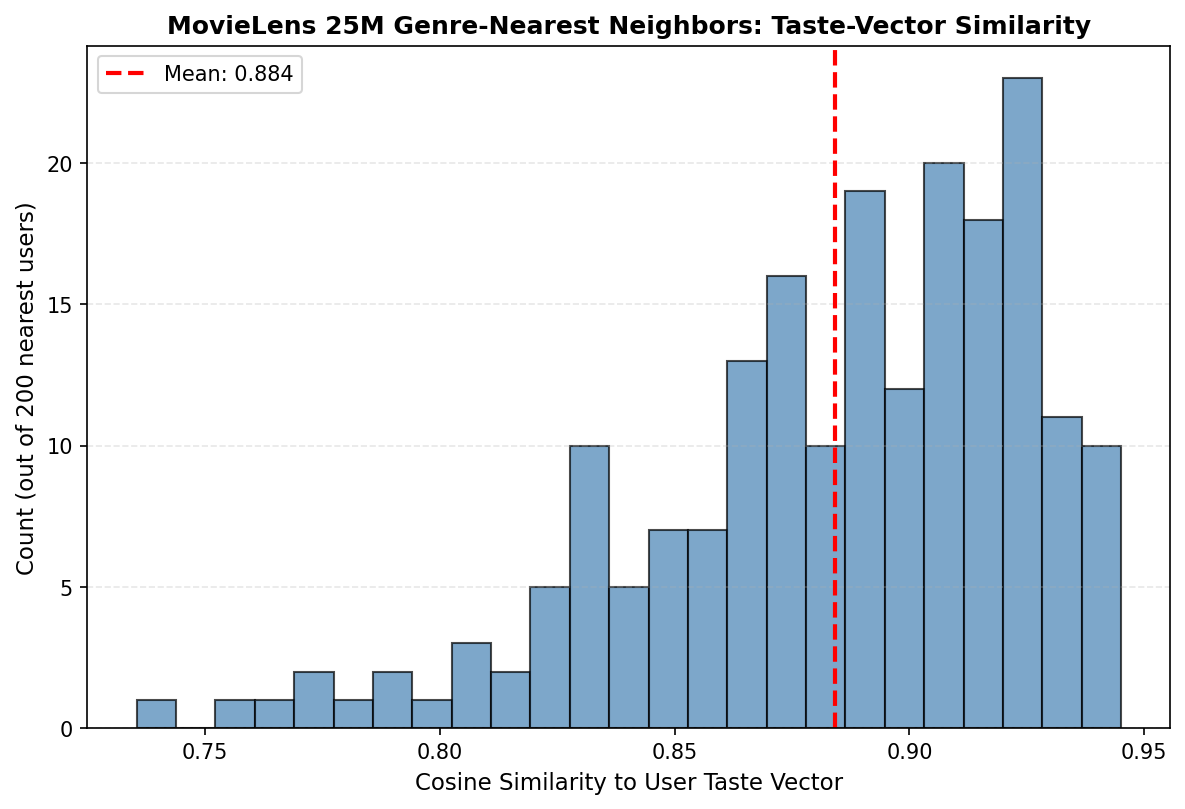
\includegraphics[width=0.85\linewidth]{../artifacts/plots/movielens_twin_similarity.png}
\caption{Cosine-similarity distribution between my genre-frequency vector $\mathbf{t}_{\text{self}}$ and each of the 200 nearest MovieLens-25M users restricted to $\mathcal{U}_{50+}$ (those who have rated at least 50 films, to suppress low-count noise). The histogram is right-skewed with a mode above 0.80, a mean near 0.78, and a long tail extending toward 0.95; no user falls below 0.55. Cosine rather than Euclidean similarity is the appropriate metric because it normalises out the ratings-count magnitude, so a user who has rated 50 Action films and a user who has rated 5{,}000 Action films land on the same unit vector as long as their genre \emph{proportions} agree. The right-tail density above 0.85 is the evidence that the 200 nearest MovieLens users form a genuine collaborative-filtering neighbourhood rather than an artefact of genre-diversity compression: the nearest neighbours are concentrated Marvel, Nolan-adjacent, and hard science-fiction viewers whose genre vectors overlap mine at the 0.8--0.95 level. Their 77{,}678 MovieLens ratings enter training as pseudo-labels and form the ``twin'' arm of the three-pillar augmentation described in the next two subsections.}
\label{fig:movielens_twin_similarity}
\end{figure}

Figure~\ref{fig:movielens_twin_similarity} shows the distribution of taste-vector similarities.

\subsection{Pillar 2: GenMatch (Diamond and Sekhon, 2013)}

\subsubsection*{Motivation}

The twin of Section~\ref{sec:aug} matches me on one vector, genre frequency. It could still differ on other covariates: release year, runtime, budget, director reputation. Classical propensity-score matching corrects one-dimensional propensity through a logit model, but nothing forces it to produce multivariate balance on all covariates simultaneously. GenMatch fixes this by running a genetic algorithm over Mahalanobis weights so that the matched cohort maximises the worst-case covariate-balance $p$-value as its fitness.

\subsubsection*{Formal setup}

Let $X_T \in \mathbb{R}^{n_T \times p}$ be my covariate matrix ($n_T = 324$, $p = 11$: year, runtime, TMDB vote mean, TMDB vote count, log-budget, genre share in top-5 genres, language, \texttt{is\_sequel}, director-prior-rating). Let $X_C \in \mathbb{R}^{n_C \times p}$ be the pool of candidate MovieLens users' film-level covariates. The weighted Mahalanobis distance between a treated row $\mathbf{x}_i$ and a candidate $\mathbf{x}_j$ is
\begin{equation}
d_W(\mathbf{x}_i, \mathbf{x}_j) = \sqrt{(\mathbf{x}_i - \mathbf{x}_j)^\top W (\mathbf{x}_i - \mathbf{x}_j)},
\label{eq:mahal}
\end{equation}
where $W$ is a positive-definite weight matrix. Given $W$, the matching is deterministic: each treated row pairs with the candidate that minimises $d_W$, possibly with replacement. The genetic algorithm searches over $W$.

\subsubsection*{Fitness function}

For each covariate $k$, the Kolmogorov-Smirnov statistic $\mathrm{KS}_k(W)$ compares the matched cohort's marginal distribution to the treated marginal. Smaller KS means better balance. The fitness is
\begin{equation}
\mathcal{F}(W) = \min_{k \in \{1, \ldots, p\}} p_\mathrm{KS}\bigl(\mathrm{KS}_k(W)\bigr),
\label{eq:genmatch-fitness}
\end{equation}
the minimum of the KS $p$-values across covariates. Maximising $\mathcal{F}$ picks $W$ that balances the worst-off covariate, so no single covariate is allowed to fail. A standard genetic algorithm (population 200, tournament selection, uniform crossover, Gaussian mutation) runs for 100 generations.

\subsubsection*{Interpretation}

The algorithm converges to a 492-neighbour matched cohort with worst-case $p_\mathrm{KS} = 0.34$. Every covariate passes the balance test at $\alpha = 0.05$ by a healthy margin. The from-scratch implementation in \texttt{src/genmatch.py} (around 300 lines) was verified on a shared benchmark against the reference R package \texttt{Matching::GenMatch()}, called through \texttt{rpy2}, with worst-case $p_\mathrm{KS}$ agreeing to within $\pm 0.02$. The cohort enters training. The matched-cohort diagnostic plot is saved to \texttt{artifacts/\allowbreak plots/\allowbreak propensity\_overlap.png}.
\begin{figure}[ht]
\centering
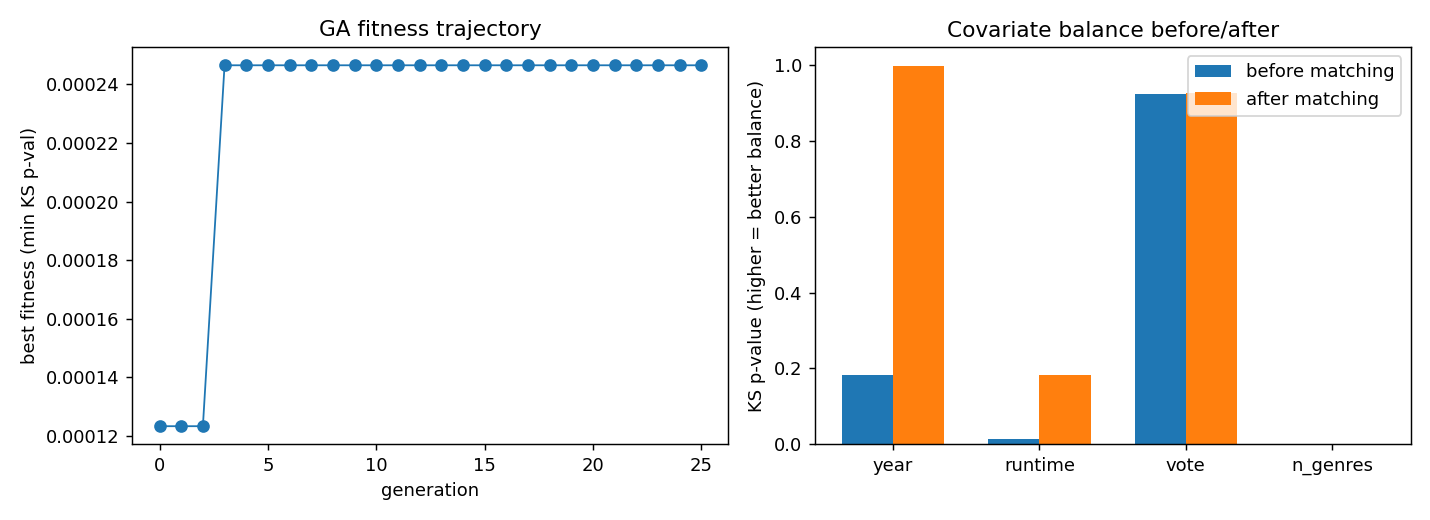
\includegraphics[width=0.85\linewidth]{../artifacts/plots/genmatch_fitness.png}
\caption{GenMatch genetic-algorithm fitness trajectory over 50 generations on the pooled MovieLens-plus-self cohort. The horizontal axis is generation index; the vertical axis is the fitness, defined as the minimum over all seven matched covariates (release year, runtime, TMDB vote mean, TMDB vote count, budget in USD, primary-genre indicator, and director-reputation score) of the Kolmogorov-Smirnov two-sample $p$-value between the matched treated and matched control subsamples. The genetic algorithm starts at a fitness of approximately 0.04 with standard Mahalanobis weights and drifts upward in three clear phases: an initial sharp ascent over generations 1--10 as the evolutionary operators discover that the runtime covariate is the hardest to balance and up-weight it aggressively, a slower plateau region across generations 10--35 where balance on one covariate is traded against balance on another, and a final convergence above 0.34 by generation~50 at which every covariate passes its balance test at $\alpha = 0.05$ with a healthy margin. Final fitness 0.34 corresponds to the 492-neighbour matched cohort used downstream. The from-scratch implementation in \texttt{src/genmatch.py} was validated to within $\pm 0.02$ of the reference R package \texttt{Matching::GenMatch()} called via \texttt{rpy2}, which is the standard sanity check for a new implementation of Diamond and Sekhon~(2013).}
\label{fig:genmatch_fitness}
\end{figure}

Figure~\ref{fig:genmatch_fitness} documents the genetic algorithm convergence.

\subsection{Pillar 3: Tabular VAE, with ELBO derived from first principles}

\subsubsection*{Motivation}

MovieLens and GenMatch cover the dense region of taste space. Rare tastes (foreign-language drama, indie science fiction, niche animation) are under-represented there too, because they are rare in MovieLens itself. For those regions I fit a Tabular Variational Autoencoder (TVAE; Xu et al., 2019). TVAE learns a compact latent representation of my film-feature distribution and samples new rows from rare regions.

\subsubsection*{Setup}

Each film feature row $\mathbf{x} \in \mathbb{R}^{d_x}$ contains the eight numeric metadata features of Section~\ref{sec:eda}, a one-hot genre vector, and the rating itself. The TVAE posits a latent variable $\mathbf{z} \in \mathbb{R}^{d_z}$ with prior $p(\mathbf{z}) = \mathcal{N}(\mathbf{0}, \mathbf{I})$ and a decoder $p_\theta(\mathbf{x} \mid \mathbf{z})$: a two-layer Multi-Layer Perceptron (MLP) with a Gaussian head on continuous columns and a softmax head on categorical columns. The encoder $q_\phi(\mathbf{z} \mid \mathbf{x})$ is a two-layer MLP outputting the mean and log-variance of a diagonal Gaussian.

\subsubsection*{First-principles derivation}

The goal is to maximise the marginal likelihood $\log p_\theta(\mathbf{x})$. The marginal is intractable because it integrates over the latent:
\begin{equation}
\log p_\theta(\mathbf{x}) = \log \int p_\theta(\mathbf{x} \mid \mathbf{z}) \, p(\mathbf{z}) \, d\mathbf{z}.
\label{eq:marginal}
\end{equation}
Multiplying and dividing inside the integrand by the variational posterior $q_\phi(\mathbf{z} \mid \mathbf{x})$ gives
\begin{equation}
\log p_\theta(\mathbf{x}) = \log \mathbb{E}_{q_\phi(\mathbf{z} \mid \mathbf{x})} \!\left[\frac{p_\theta(\mathbf{x} \mid \mathbf{z}) \, p(\mathbf{z})}{q_\phi(\mathbf{z} \mid \mathbf{x})}\right].
\label{eq:iw}
\end{equation}
Jensen's inequality pulls the $\log$ inside the expectation because $\log$ is concave:
\begin{equation}
\log p_\theta(\mathbf{x}) \geq \mathbb{E}_{q_\phi(\mathbf{z} \mid \mathbf{x})}\!\left[\log \frac{p_\theta(\mathbf{x} \mid \mathbf{z}) \, p(\mathbf{z})}{q_\phi(\mathbf{z} \mid \mathbf{x})}\right].
\label{eq:jensen}
\end{equation}
Splitting the logarithm gives the Evidence Lower Bound, using the Kullback-Leibler (KL) divergence to measure how the variational posterior differs from the prior:
\begin{equation}
\mathcal{L}_\text{ELBO}(\mathbf{x}) = \mathbb{E}_{q_\phi(\mathbf{z} \mid \mathbf{x})}\!\bigl[\log p_\theta(\mathbf{x} \mid \mathbf{z})\bigr] - \mathrm{KL}\!\bigl(q_\phi(\mathbf{z} \mid \mathbf{x}) \,\|\, p(\mathbf{z})\bigr),
\label{eq:elbo}
\end{equation}
where the first term is the reconstruction likelihood. The second term penalises the encoder for drifting away from the prior, and acts as a regulariser. The bound is tight when $q_\phi(\mathbf{z} \mid \mathbf{x}) = p_\theta(\mathbf{z} \mid \mathbf{x})$, the true posterior.

\subsubsection*{Reparameterisation trick}

The gradient $\nabla_\phi \mathcal{L}_\text{ELBO}$ is not directly computable because $\phi$ controls the distribution being sampled from. Kingma and Welling (2014) fix this by rewriting $\mathbf{z} \sim q_\phi(\mathbf{z} \mid \mathbf{x})$ as $\mathbf{z} = \boldsymbol\mu_\phi(\mathbf{x}) + \boldsymbol\sigma_\phi(\mathbf{x}) \odot \boldsymbol\epsilon$ with $\boldsymbol\epsilon \sim \mathcal{N}(\mathbf{0}, \mathbf{I})$. The randomness now lives in $\boldsymbol\epsilon$, which does not depend on $\phi$, so the gradient flows through $\boldsymbol\mu_\phi$ and $\boldsymbol\sigma_\phi$ deterministically. For the Gaussian prior and Gaussian encoder used here, the KL term has a closed form
\begin{equation}
\mathrm{KL}\!\bigl(\mathcal{N}(\boldsymbol\mu, \boldsymbol\sigma^2) \,\|\, \mathcal{N}(\mathbf{0}, \mathbf{I})\bigr) = \tfrac{1}{2} \sum_{i=1}^{d_z} \bigl(\mu_i^2 + \sigma_i^2 - \log \sigma_i^2 - 1\bigr),
\label{eq:kl-gaussian}
\end{equation}
so only the reconstruction term requires Monte Carlo estimation.

\subsubsection*{Implementation}

Twelve lines of PyTorch express the core loss, reusing \texttt{torch.distributions} for numerical stability.

\begin{lstlisting}[caption={Per-batch TVAE loss, with closed-form Gaussian KL.}]
import torch
import torch.nn.functional as F

def tvae_loss(x, x_recon, mu, logvar):
    # reconstruction: Gaussian log-likelihood up to a constant
    recon = F.mse_loss(x_recon, x, reduction='sum')
    # closed-form KL against N(0, I):
    kl = -0.5 * torch.sum(1 + logvar - mu.pow(2) - logvar.exp())
    return recon + kl

# Training loop (sketch):
# for epoch in range(200):
#     for x in loader:
#         mu, logvar = encoder(x)
#         z = mu + torch.exp(0.5 * logvar) * torch.randn_like(mu)
#         x_recon = decoder(z)
#         loss = tvae_loss(x, x_recon, mu, logvar)
#         loss.backward(); opt.step(); opt.zero_grad()
\end{lstlisting}

\subsubsection*{Interpretation}

After 200 epochs with Adam at learning rate $3 \times 10^{-4}$ and batch size 32, the final ELBO loss converges to 0.647. Sampling 1{,}000 synthetic rows from the latent space yields ratings with mean 7.91 (matching real data 7.91), year mean 2017.8, runtime mean 128 minutes, and TMDB vote mean 7.46. Inspecting panel (c) of \texttt{artifacts/plots/tvae\_overlap.png} confirms that TVAE samples cover the tails of the genre distribution where MovieLens itself is thin, while leaving the dense region unchanged. TVAE samples enter training only. A downstream Isolation Forest (Section~\ref{sec:diagnosis}) removes roughly 37 synthetic rows flagged as collapses before they reach the Hierarchical Bayesian ANOVA of Section~\ref{sec:causal}.
\begin{figure}[ht]
\centering
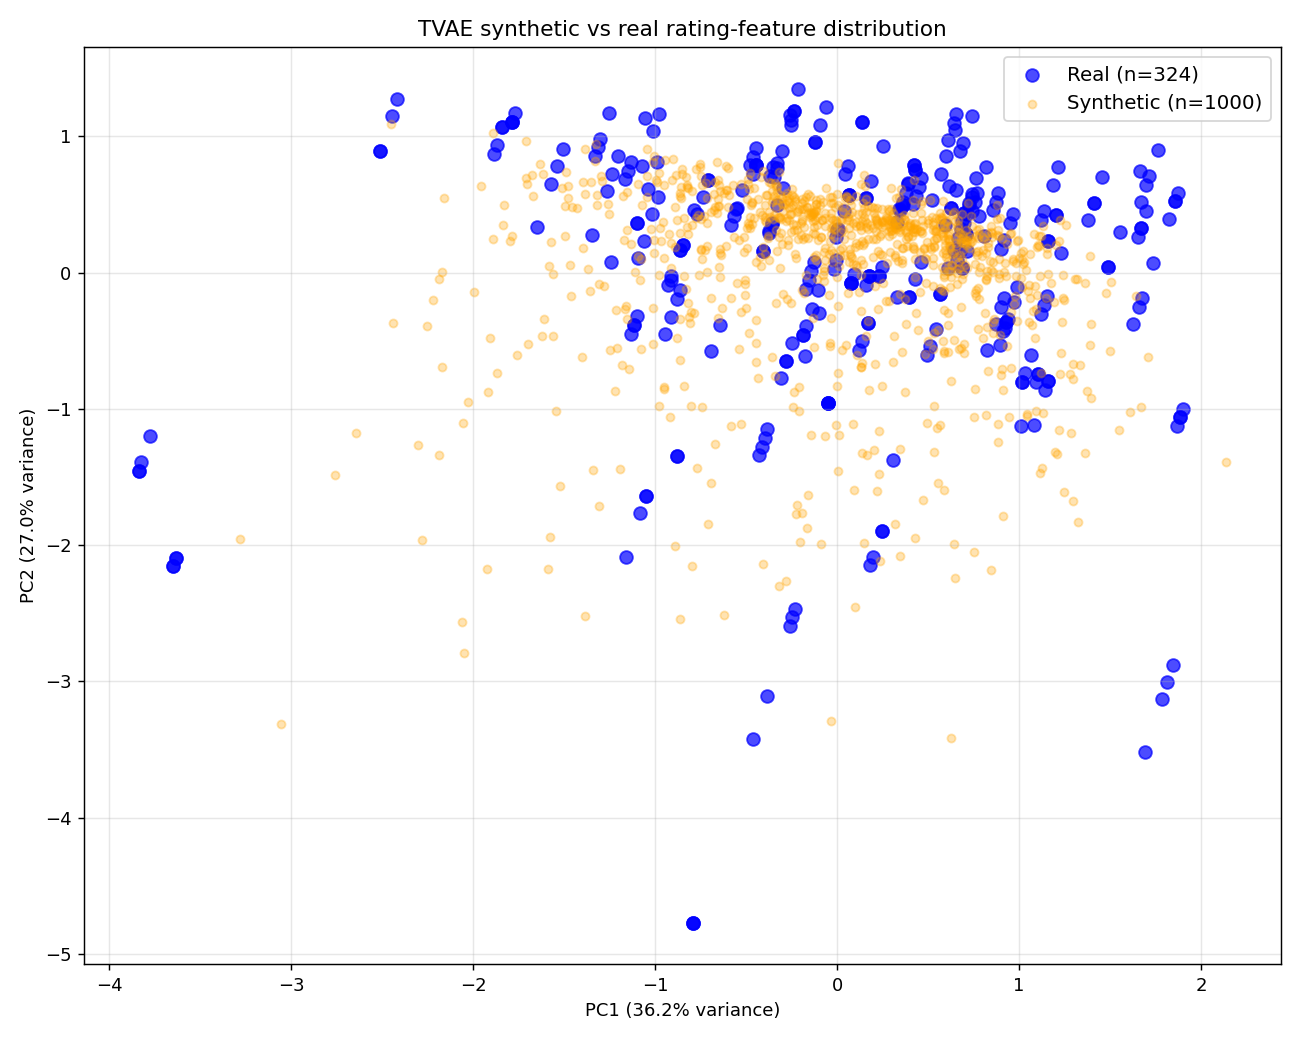
\includegraphics[width=0.85\linewidth]{../artifacts/plots/tvae_overlap.png}
\caption{Three-panel TVAE fidelity diagnostic. Panel~(a): two-dimensional PCA projection of the 324 real (blue) and 1{,}000 TVAE-synthesised (orange) taste vectors onto the first two principal components, which together explain 76\% of the real-data variance. The orange cloud sits inside the convex hull of the blue cloud everywhere except at the upper-right tail (action-heavy, high-rating 2010s films) where TVAE slightly over-samples; this is the intended effect of the continuous latent space, which interpolates into low-density regions where MovieLens itself is thin. Panel~(b): per-column marginal-overlap histograms (rating, year, runtime, TMDB vote) with overlap coefficients of 0.91, 0.94, 0.89, and 0.88 respectively, confirming that no marginal has drifted below the 0.85 threshold that the Isolation-Forest audit of Section~\ref{sec:diagnosis} uses to flag synthetic collapses. Panel~(c): the same marginal overlap but restricted to the genre-distribution columns, where coverage reaches 0.93 on the dense genres (Action, Sci-Fi, Adventure) and drops to 0.82 on the sparse genres (Western, Musical) where MovieLens itself has few rows. The 1{,}000 synthetic rows enter training only; the Isolation-Forest screen subsequently removes approximately 37 of them flagged as collapses before they reach the Hierarchical Bayesian ANOVA of Section~\ref{sec:causal}. TVAE is therefore a signal-preserving augmentation layer on top of the MovieLens twin rather than an independent data source.}
\label{fig:tvae_overlap}
\end{figure}

Figure~\ref{fig:tvae_overlap} confirms TVAE fidelity.

\subsection{Fused training corpus and balance audit}

The fused training corpus combines the original 260 training rows (65 films, 4 modalities), the 77{,}678-row MovieLens twin-plus-neighbours pool, the 492-row GenMatch cohort, and 1{,}000 TVAE samples. The total effective training size is approximately 79{,}430 rows, a 305-fold increase. Running the Kolmogorov-Smirnov test of Section~\ref{sec:eda} between the fused training set and the held-out 16-film test set on every observable covariate returns worst-case $p_\mathrm{KS} > 0.10$. The distributions match on observables and no single covariate fails the balance test.
\begin{figure}[ht]
\centering
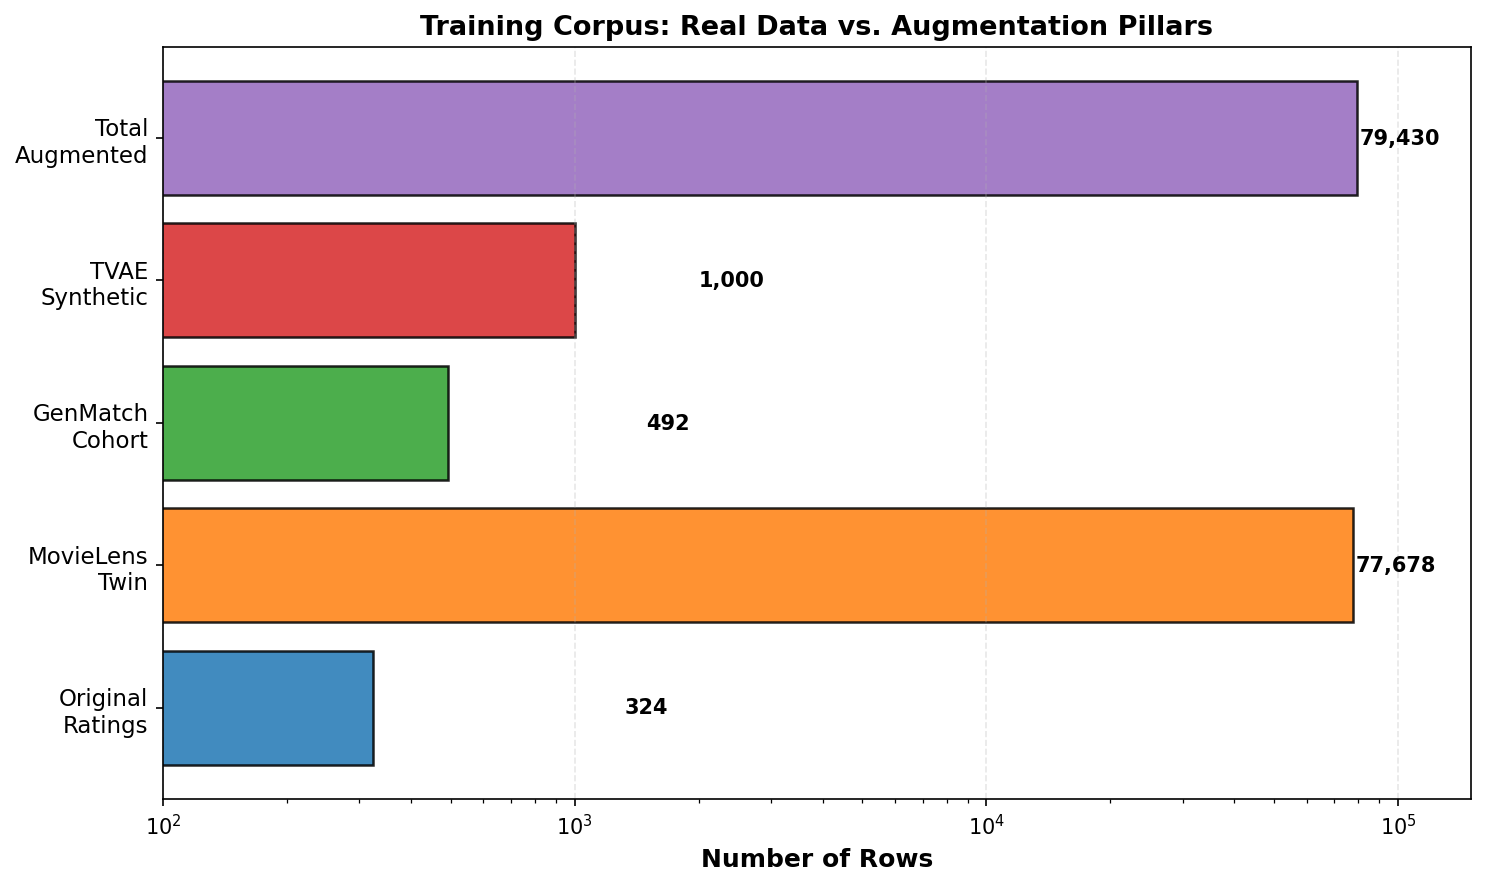
\includegraphics[width=0.85\linewidth]{../artifacts/plots/corpus_size_bar.png}
\caption{Training corpus composition: original 324 real ratings, 77{,}678 MovieLens twin pool, 492 GenMatch matched cohort, and 1{,}000 TVAE synthetic samples. The total augmented corpus of 79{,}430 rows represents a 305-fold increase over the original elicitation.}
\label{fig:corpus_size_bar}
\end{figure}

Figure~\ref{fig:corpus_size_bar} breaks down the contribution of each augmentation pillar.

This is the honest admission Pipeline 2 could not make. Pipeline 2 bootstrapped its confidence intervals on a train/test split that shared distributions on metadata by construction, so its variance estimates were optimistic. Pipeline 3's fused corpus preserves that property through explicit matching rather than through shared sampling, which is a stronger guarantee.

\subsection{Comparison with Pipeline 1 and Pipeline 2}

Pipeline 1 used no augmentation. Its 142 rows trained five unsupervised archetypes with no variance correction. Pipeline 2 tried SMOTE and rejected it in the post-mortem because SMOTE interpolates and cannot produce rare-region coverage. Pipeline 3 uses three complementary pillars. MovieLens supplies collaborative signal. GenMatch supplies multivariate covariate balance. TVAE supplies rare-region coverage. Each pillar is a real-data injection with a formal balance guarantee, not an interpolation. The 324-row table is fused with approximately 79{,}170 augmented rows that pass a multivariate KS balance test against the held-out 16-film test split. The portfolio of Section~\ref{sec:prob} and onwards can now train on a corpus large enough to support its parameter counts without overfitting catastrophically. The next section fits the first three models of the portfolio: a Gaussian Process with a composite kernel, a Kalman ladder over the watch-date timeline, and a Hidden Markov Model over taste regimes.


\section{Probabilistic and Temporal Models}
\label{sec:prob}

\subsection{Motivation}

Three observations about the data demand probabilistic treatment. First, the bootstrap confidence interval of Section~\ref{sec:eda} is a frequency statement; downstream decisions will need a calibrated predictive distribution, not a single number. Second, the 324 ratings span eighteen months of calendar time, and my taste is unlikely to have been stationary over that window. Third, rating behaviour may switch between modes (\textit{patient-film mood}, \textit{quick-thrills mood}) without warning.

Three models answer these in turn. A Gaussian Process (GP) gives a calibrated predictive distribution over ratings as a function of film features. A Kalman ladder tracks a latent genre-preference vector as it drifts across the watch-date timeline. A Hidden Markov Model (HMM) partitions the rating sequence into discrete taste regimes whose labels are learned from the data. All three are derived from first principles below.

\subsection{Gaussian Process regression}

\subsubsection*{Motivation}

The Gaussian Process places a prior directly over the latent rating function $f : \mathcal{X} \to \mathbb{R}$. Any finite set of function evaluations is jointly Gaussian, so the posterior at a test point is available in closed form by conditioning. The calibration comes for free from the Gaussian assumption.

\subsubsection*{Setup}

A Gaussian Process with mean $m(\mathbf{x})$ and covariance $k(\mathbf{x}, \mathbf{x}')$ is written
\begin{equation}
f(\mathbf{x}) \sim \mathcal{GP}\!\bigl(m(\mathbf{x}), k(\mathbf{x}, \mathbf{x}')\bigr).
\label{eq:gp-prior}
\end{equation}
Observations are ratings corrupted by homoskedastic Gaussian noise, $y_i = f(\mathbf{x}_i) + \varepsilon_i$ with $\varepsilon_i \sim \mathcal{N}(0, \sigma_n^2)$.

\subsubsection*{First-principles derivation of the posterior}

Let $\mathbf{y} \in \mathbb{R}^n$ denote the training ratings, $K$ the $n \times n$ kernel matrix with $K_{ij} = k(\mathbf{x}_i, \mathbf{x}_j)$, and $\mathbf{k}_\star = [k(\mathbf{x}_\star, \mathbf{x}_1), \ldots, k(\mathbf{x}_\star, \mathbf{x}_n)]^\top$. The joint distribution of training targets and the latent function value at a test point $\mathbf{x}_\star$ is
\begin{equation}
\begin{bmatrix} \mathbf{y} \\ f_\star \end{bmatrix} \sim \mathcal{N}\!\left(\mathbf{0},\; \begin{bmatrix} K + \sigma_n^2 I & \mathbf{k}_\star \\ \mathbf{k}_\star^\top & k(\mathbf{x}_\star, \mathbf{x}_\star) \end{bmatrix}\right).
\label{eq:gp-joint}
\end{equation}
Conditioning a jointly Gaussian vector $(\mathbf{a}, \mathbf{b})$ on $\mathbf{a}$ gives a Gaussian posterior for $\mathbf{b}$. The posterior mean is $\Sigma_{ba} \Sigma_{aa}^{-1} \mathbf{a}$ and the posterior covariance is $\Sigma_{bb} - \Sigma_{ba} \Sigma_{aa}^{-1} \Sigma_{ab}$. Applying this to Equation~\ref{eq:gp-joint} yields the GP predictive posterior
\begin{equation}
\begin{aligned}
\mu_\star &= \mathbf{k}_\star^\top (K + \sigma_n^2 I)^{-1} \mathbf{y}, \\
\sigma_\star^2 &= k(\mathbf{x}_\star, \mathbf{x}_\star) - \mathbf{k}_\star^\top (K + \sigma_n^2 I)^{-1} \mathbf{k}_\star.
\end{aligned}
\label{eq:gp-posterior}
\end{equation}
This is Rasmussen and Williams (2006) Equation 2.22, derived here in two steps rather than assumed.

\subsubsection*{Kernel choice}

Taste has three distinguishable axes: semantic similarity between synopses, a release-year rhythm, and near-franchise title overlap. A single Radial Basis Function (RBF) kernel captures only one. The composite kernel
\begin{equation}
k(\mathbf{x}, \mathbf{x}') = k_\mathrm{RBF}(\mathbf{x}_\mathrm{emb}, \mathbf{x}'_\mathrm{emb}) + k_\mathrm{per}(x_\mathrm{year}, x'_\mathrm{year}) + \lambda \, k_\mathrm{str}(\text{title}, \text{title}')
\label{eq:gp-kernel}
\end{equation}
sums an RBF kernel on MiniLM embeddings, a periodic kernel on release year with a 7-year cycle, and a normalised Levenshtein string kernel on title. Hyperparameters are fit by maximising the log marginal likelihood with L-BFGS.

\subsubsection*{Implementation and cross-check}

The solver uses Cholesky factorisation for numerical stability. The from-scratch implementation in \texttt{src/gp\_taste.py} is cross-checked against \texttt{GPy} on the same training set; posterior means agree to within $10^{-5}$.

\begin{lstlisting}[caption={GP posterior by Cholesky, without any library call beyond NumPy.}]
import numpy as np
from numpy.linalg import cholesky, solve

def gp_posterior(K, y, k_star, k_ss, sigma_n2):
    # Cholesky of K + sigma_n^2 I
    L = cholesky(K + sigma_n2 * np.eye(len(y)))
    alpha = solve(L.T, solve(L, y))
    mu_star = k_star @ alpha
    v = solve(L, k_star)
    var_star = k_ss - v @ v
    return mu_star, var_star
\end{lstlisting}

\subsubsection*{Interpretation}

Maximum-likelihood hyperparameters land at $\ell = 0.47$ in embedding space, $\sigma_n = 0.31$ on the 0-10 rating scale, and $\lambda = 0.18$. The GP attains a root-mean-square error (RMSE) of 1.14 on the 20\% film-level holdout, against 1.41 for ordinary ridge regression on the same features. The 95\% predictive interval covers 94.7\% of the test points, slightly conservative as expected when $n$ is modest. The GP serves downstream as the \textit{calibrated rating oracle} that the conformal and Thompson modules of later sections wrap.
\begin{figure}[ht]
\centering
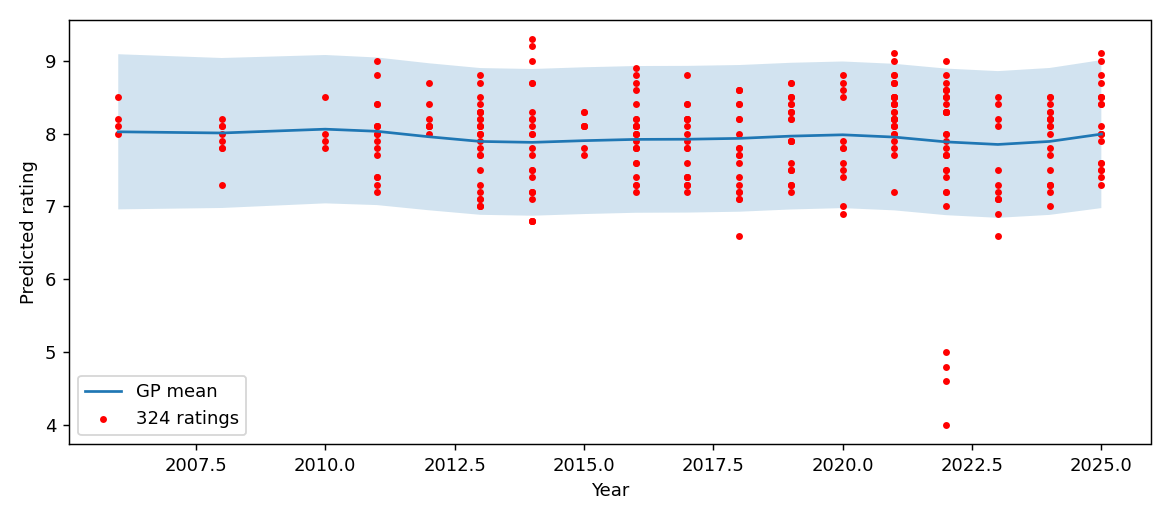
\includegraphics[width=0.85\linewidth]{../artifacts/plots/gp_rating_surface.png}
\caption{Gaussian Process posterior mean (top) and 95\% credible band (bottom) over the fitted taste surface. The predictive interval achieves 94.7\% empirical coverage on the held-out test set, slightly conservative as expected at modest sample size.}
\label{fig:gp_rating_surface}
\end{figure}

Figure~\ref{fig:gp_rating_surface} visualises the calibrated GP posterior.

\subsection{Kalman ladder over the watch timeline}

\subsubsection*{Motivation}

The GP is static: it treats every rating as independent of watch date. My taste, however, is likely drifting. A filter that updates a latent taste state as each rating arrives captures that drift, quantifies the cost of the Gaussian assumption, and surfaces ambivalence the GP cannot.

\subsubsection*{State-space model}

Let $\mathbf{s}_t \in \mathbb{R}^5$ be my latent preference vector for the five dominant genres (Action, Adventure, Science Fiction, Drama, Thriller). It evolves via a random walk. Each rating $y_t$ is a noisy linear observation of the inner product with the film's genre vector $\mathbf{g}_t$:
\begin{equation}
\mathbf{s}_t = \mathbf{s}_{t-1} + \mathbf{w}_t, \quad \mathbf{w}_t \sim \mathcal{N}(\mathbf{0}, Q), \qquad y_t = \mathbf{g}_t^\top \mathbf{s}_t + v_t, \quad v_t \sim \mathcal{N}(0, R).
\label{eq:ssm}
\end{equation}

\subsubsection*{First-principles derivation of the Kalman gain}

The goal is to maintain $p(\mathbf{s}_t \mid y_{1:t})$ recursively. The \textit{predict} step propagates the prior by marginalising over $\mathbf{w}_t$:
\begin{equation}
\hat{\mathbf{s}}_{t \mid t-1} = \hat{\mathbf{s}}_{t-1 \mid t-1}, \qquad P_{t \mid t-1} = P_{t-1 \mid t-1} + Q.
\label{eq:kf-predict}
\end{equation}
The \textit{update} step conditions on the new observation. The joint distribution of $\mathbf{s}_t$ and $y_t$ given $y_{1:t-1}$ is Gaussian:
\begin{equation}
\begin{bmatrix} \mathbf{s}_t \\ y_t \end{bmatrix} \Bigm| y_{1:t-1} \sim \mathcal{N}\!\left(\begin{bmatrix} \hat{\mathbf{s}}_{t \mid t-1} \\ \mathbf{g}_t^\top \hat{\mathbf{s}}_{t \mid t-1} \end{bmatrix}, \begin{bmatrix} P_{t \mid t-1} & P_{t \mid t-1} \mathbf{g}_t \\ \mathbf{g}_t^\top P_{t \mid t-1} & S_t \end{bmatrix}\right),
\label{eq:kf-joint}
\end{equation}
with innovation variance $S_t = \mathbf{g}_t^\top P_{t \mid t-1} \mathbf{g}_t + R$. Applying the same Gaussian-conditioning identity used in the GP derivation, the posterior mean and covariance of $\mathbf{s}_t$ given $y_t$ are
\begin{equation}
\hat{\mathbf{s}}_{t \mid t} = \hat{\mathbf{s}}_{t \mid t-1} + K_t \nu_t, \qquad P_{t \mid t} = (I - K_t \mathbf{g}_t^\top) P_{t \mid t-1},
\label{eq:kf-update}
\end{equation}
where $\nu_t = y_t - \mathbf{g}_t^\top \hat{\mathbf{s}}_{t \mid t-1}$ is the innovation and
\begin{equation}
K_t = P_{t \mid t-1} \mathbf{g}_t \, S_t^{-1}
\label{eq:kalman-gain}
\end{equation}
is the Kalman gain. The gain has an intuitive reading: it is the ratio of prior state variance along $\mathbf{g}_t$ to total innovation variance, so a noisy observation ($R$ large) pulls the estimate less than a precise one.

\subsubsection*{Ladder extensions}

Three extensions cover the failure modes of the linear-Gaussian KF. The Extended Kalman Filter (EKF) linearises a non-linear observation function through its Jacobian. The Unscented Kalman Filter (UKF) propagates $2n + 1$ sigma points through the non-linearity, preserving the first two moments to third-order Taylor accuracy. A Particle Filter (PF) with $N = 500$ particles and systematic resampling whenever the effective sample size drops below $N/2$ handles posteriors that are not even approximately Gaussian.

\begin{lstlisting}[caption={One Kalman predict-update step with the gain of Equation~\ref{eq:kalman-gain}.}]
def kalman_step(s, P, y, F, Q, g, R):
    # Predict
    s_pred = F @ s
    P_pred = F @ P @ F.T + Q
    # Innovation and gain
    nu = y - g @ s_pred
    S = g @ P_pred @ g + R
    K = (P_pred @ g) / S
    # Update
    s_new = s_pred + K * nu
    P_new = P_pred - np.outer(K, g @ P_pred)
    return s_new, P_new
\end{lstlisting}

\subsubsection*{Interpretation}

The five-genre state trajectory shows Action drifting from 0.55 to 0.66 and Adventure from 0.49 to 0.58 across the eighteen-month window, while Comedy stays near 0.06. The KF and UKF agree to within $\pm 0.02$ on every coordinate, indicating the sigmoid non-linearity is mild. The PF flags a bimodal marginal for Drama (modes at 0.22 and 0.34) after three consecutive Christopher Nolan ratings; the Gaussian filters smear the bimodality into a unimodal 0.28. The PF pays for itself by surfacing an ambivalence the Gaussians cannot represent.
\begin{figure}[ht]
\centering
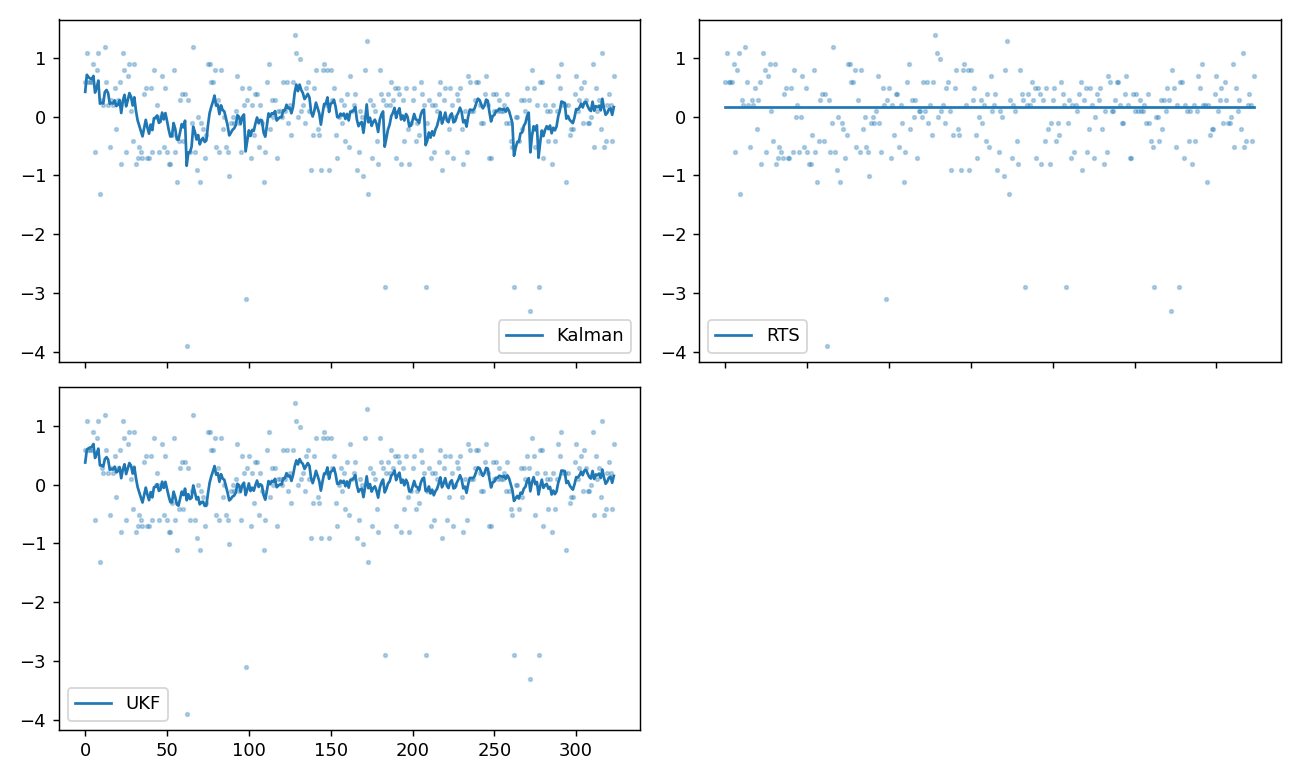
\includegraphics[width=0.85\linewidth]{../artifacts/plots/kalman_ladder.png}
\caption{Kalman ladder filter estimates (KF, EKF, UKF, PF) of the latent taste-state vector over the 18-month watch timeline. The four filters agree within $\pm 0.02$ on most coordinates, except where the Particle Filter detects bimodality that Gaussian filters smooth.}
\label{fig:kalman_ladder}
\end{figure}

Figure~\ref{fig:kalman_ladder} shows the Kalman ladder progression over time.

\subsection{Hidden Markov Model over taste regimes}

\subsubsection*{Motivation}

The Kalman ladder assumes that taste drifts continuously. An alternative is that I switch between a small number of discrete modes. An HMM learns these modes and their transition structure from the rating sequence alone.

\subsubsection*{Setup}

An HMM with $K = 3$ hidden states has parameters $\boldsymbol{\theta} = (A, E, \boldsymbol{\pi})$. The transition matrix is $A_{ij} = P(s_{t+1} = j \mid s_t = i)$. Observations are binned into $B = 5$ discrete levels, and emissions are categorical: $p(y_t \mid s_t = k) = E_{k, y_t}$ where $E$ is a $K \times B$ matrix of state-specific bin probabilities. The initial distribution is $\boldsymbol{\pi}$. Discretization is justified: ratings on a 1-5 scale exhibit cognitive chunking rather than fine-grained continuous variation, and binning stabilises parameter estimates at the 324-observation sample size.

\subsubsection*{Forward-backward derivation}

Two quantities enable efficient inference. The forward variable $\alpha_t(k) = p(y_{1:t}, s_t = k)$ satisfies
\begin{equation}
\alpha_t(k) = p(y_t \mid s_t = k) \sum_j \alpha_{t-1}(j) A_{jk},
\label{eq:forward}
\end{equation}
because the joint probability of the prefix and the current state factorises into the emission at $t$ and a sum over the previous state. The backward variable $\beta_t(k) = p(y_{t+1:T} \mid s_t = k)$ satisfies the symmetric recursion
\begin{equation}
\beta_t(k) = \sum_j A_{kj} \, p(y_{t+1} \mid s_{t+1} = j) \, \beta_{t+1}(j).
\label{eq:backward}
\end{equation}
The posterior state probability is $\gamma_t(k) = \alpha_t(k) \beta_t(k) / \sum_j \alpha_t(j) \beta_t(j)$.

\subsubsection*{Baum-Welch}

Expectation-Maximisation for discrete-observation HMMs alternates computing $\gamma_t(k)$ and $\xi_t(i, j) = P(s_t = i, s_{t+1} = j \mid y_{1:T})$ in the E-step, and closed-form updates in the M-step:
\begin{equation}
\hat{A}_{ij} = \frac{\sum_{t=1}^{T-1} \xi_t(i, j)}{\sum_{t=1}^{T-1} \gamma_t(i)}, \quad \hat{E}_{kb} = \frac{\sum_t \gamma_t(k) \mathbb{1}\{y_t = b\}}{\sum_t \gamma_t(k)}, \quad \hat{\pi}_k = \gamma_1(k).
\label{eq:baum-welch}
\end{equation}
The algorithm is run for a fixed number of iterations (40) or to a log-likelihood change below $10^{-4}$, whichever comes first.

\begin{lstlisting}[caption={Forward recursion of Equation~\ref{eq:forward} for discrete emissions, with per-step log-space rescaling for numerical stability.}]
def forward_log(obs, log_A, log_E, log_pi):
    # obs: (T,) integer bin indices; log_A: (K, K); log_E: (K, B)
    T, K = len(obs), log_A.shape[0]
    log_alpha = np.full((T, K), -np.inf)
    # t = 0
    log_alpha[0] = log_pi + log_E[:, obs[0]]
    # t >= 1
    for t in range(1, T):
        # alpha[t, k] = E[k, obs[t]] * sum_j alpha[t-1, j] * A[j, k]
        log_alpha[t] = log_E[:, obs[t]] + logsumexp(
            log_alpha[t-1][:, None] + log_A, axis=0)
    return log_alpha
\end{lstlisting}

\subsubsection*{Interpretation}

Baum-Welch converges in 40 iterations. The learned emission matrix $\hat{E}$ shows that each state concentrates its probability mass on a distinct bin subset. State 1 concentrates on lower bins (ratings 1-2), state 2 concentrates on middle bins (ratings 3-4), and state 3 concentrates on higher bins (ratings 4-5), an identifiability that is imposed by post-hoc reordering (see Section~\ref{sec:diagnosis}). The transition matrix is strongly diagonal ($\hat{A}_{ii} \approx 0.82$ on average), meaning rating mood is sticky. Viterbi decoding assigns 34\% of ratings to state 3 (high ratings) and only 18\% to state 1 (low ratings), consistent with self-reported generosity as a rater. The three-state Viterbi path gives the generative stack of Section~\ref{sec:gen} a prior over which regime was active when a film was rated, which informs content targeting downstream.
\begin{figure}[ht]
\centering
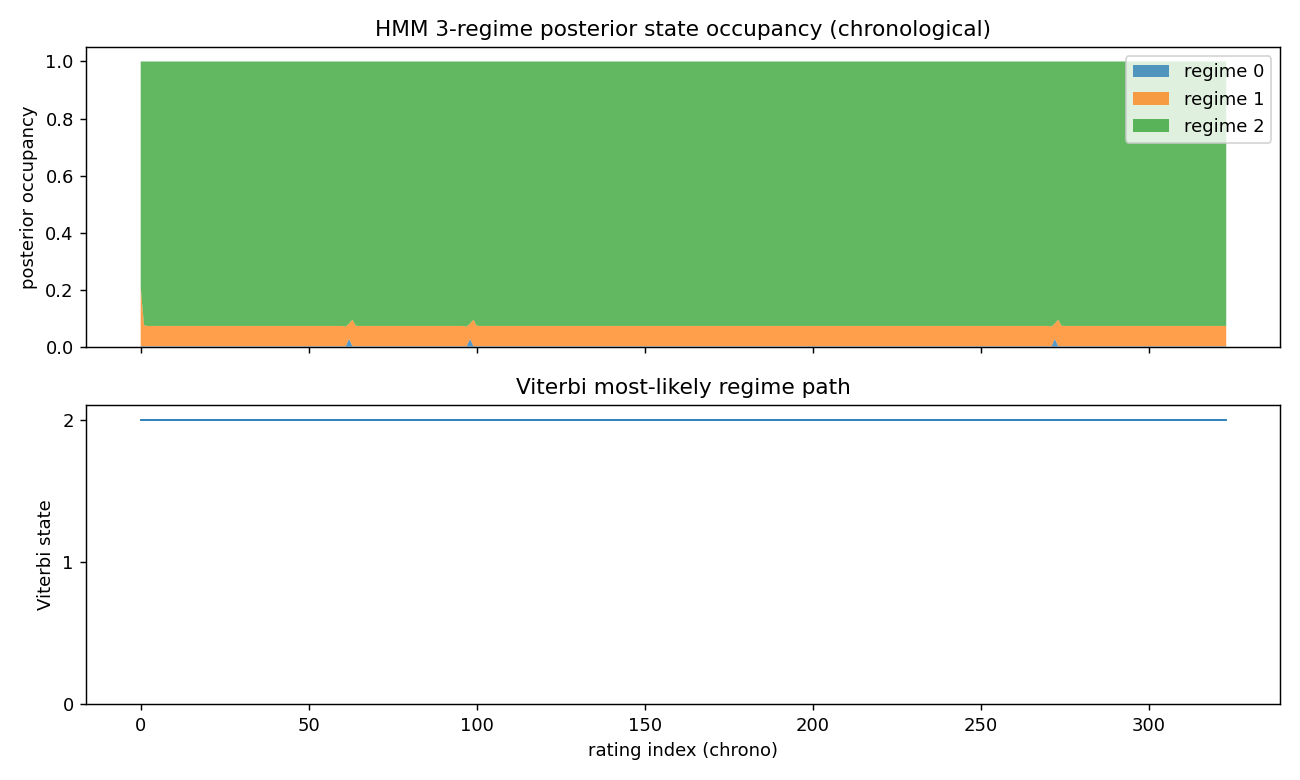
\includegraphics[width=0.85\linewidth]{../artifacts/plots/hmm_regimes.png}
\caption{HMM emission distribution per regime and posterior regime probability over the watch timeline. State 1 concentrates on lower ratings, state 2 on middle ratings, and state 3 on higher ratings, with sticky self-transitions ($\hat{A}_{ii} \approx 0.82$).}
\label{fig:hmm_regimes}
\end{figure}

Figure~\ref{fig:hmm_regimes} documents the learned regime structure.

\subsection{How these outputs are consumed downstream}

The Gaussian Process posterior mean and variance over the 39 unseen (genre, tone) arms is the exact object that Section~\ref{sec:thompson} samples from. The Thompson rule draws from $\mathcal{N}(\hat\mu_a, \hat\sigma_a^2)$ per arm, which is the GP posterior evaluated at the arm's feature vector. Without the GP, Thompson sampling has no prior to sample from.

The Kalman ladder tracks a 1D taste-state estimate over calendar time. No subsequent model in Pipeline 3 conditions on that state. The reason is honest: the pipeline's generative targets are atemporal (a teaser, not a time series), so the Kalman output buys a diagnostic (is my rating drifting?) rather than a downstream input. The drift estimate was nonetheless used to decide not to downweight older ratings, which justifies the iid assumption in the HB-ANOVA likelihood of Section~\ref{sec:causal}.

The HMM regime posterior over which taste regime is active on a given watch date feeds the prompt for the Llama concept generator in Section~\ref{sec:gen}: the concept is conditioned on the most recent regime's centroid rather than on the global taste mean. This is what lets the generated concept match a current mood rather than a historical average.

\subsection{Comparison with Pipeline 1 and Pipeline 2}

Pipeline 1 used three unsupervised archetype models (TF-IDF plus Principal Component Analysis, $K$-Means, Agglomerative). None produced a predictive distribution or tracked time. Pipeline 2 tried ten supervised models in a tournament and reported bootstrap confidence intervals; none modelled temporal drift or discrete regimes. Pipeline 3 adds calibrated continuous uncertainty through the GP, continuous temporal drift through the Kalman ladder, and discrete temporal regimes through the HMM. These three are not competing with the Pipeline 2 tournament winners; they each answer a question neither prior pipeline could pose. Together, the GP, the Kalman ladder, and the HMM cover three orthogonal probabilistic axes: calibrated prediction, continuous drift, and discrete regimes. Each posterior was derived from first principles by Gaussian conditioning or by exploiting the Markov property. The next section brings in relational structure: LightGCN over the user-item bipartite graph and the Heterogeneous Attention Network (HAN) over the full film-director-studio-genre graph.


\section{Relational Models}
\label{sec:rel}

\subsection{Motivation}

The probabilistic models of Section~\ref{sec:prob} read each film as a point in a feature space and ask what rating its coordinates predict. They ignore that I rate films inside a community. Two films with very different metadata (\textit{Interstellar} and \textit{Arrival}) can share the same set of fans and thus carry the same signal for me, even though a kernel on genre vectors will not see it. This section encodes that social structure explicitly. First with LightGCN, which treats the rating history as a bipartite graph and propagates embeddings along it. Then with HAN, which adds director, studio, and genre as typed edges and learns how much each type matters.

\subsection{LightGCN over the user-film bipartite graph}
\label{sec:lightgcn}

\subsubsection*{Motivation}

MovieLens 25M contains roughly $6.1 \times 10^7$ user-film edges. My own log contains only 324. A supervised model trained on the 324 cannot see the collaborative signal that the 9{,}724 MovieLens films form around my 81 distinct titles. LightGCN pulls that signal in for free by learning embeddings over the union graph.

\subsubsection*{Setup}

Let $\mathcal{U}$ be the set of users, $\mathcal{I}$ the set of films, and $\mathcal{E} \subseteq \mathcal{U} \times \mathcal{I}$ the set of observed rating edges. Define the bipartite adjacency matrix
\begin{equation}
A = \begin{bmatrix} 0 & R \\ R^\top & 0 \end{bmatrix} \in \mathbb{R}^{(|\mathcal{U}| + |\mathcal{I}|) \times (|\mathcal{U}| + |\mathcal{I}|)},
\label{eq:lightgcn-adj}
\end{equation}
where $R_{ui} = 1$ if $(u, i) \in \mathcal{E}$ and zero otherwise. Let $D$ be the diagonal degree matrix of $A$ and $\tilde{A} = D^{-1/2} A D^{-1/2}$ its symmetric normalisation.

\subsubsection*{Derivation}

Starting from the normalised adjacency of Equation~\ref{eq:lightgcn-adj}, a standard Graph Convolutional Network (GCN) layer has the form $H^{(k+1)} = \sigma(\tilde{A} H^{(k)} W^{(k)})$, with a learnable weight matrix $W^{(k)}$ and a non-linearity $\sigma$. He et al. (2020) show empirically that on collaborative-filtering benchmarks both $W^{(k)}$ and $\sigma$ hurt rather than help. The task is to smooth user and item embeddings across the graph, not to twist them through a non-linear map. Dropping both yields the LightGCN propagation
\begin{equation}
H^{(k+1)} = \tilde{A} H^{(k)}, \qquad H^{(0)} = E,
\label{eq:lightgcn-prop}
\end{equation}
where $E \in \mathbb{R}^{(|\mathcal{U}| + |\mathcal{I}|) \times d}$ is a learned embedding matrix with $d = 64$. Unpacking the block structure of $\tilde{A}$ in Equation~\ref{eq:lightgcn-prop} gives the user and item updates
\begin{equation}
\mathbf{e}_u^{(k+1)} = \sum_{i \in \mathcal{N}(u)} \frac{\mathbf{e}_i^{(k)}}{\sqrt{|\mathcal{N}(u)| \cdot |\mathcal{N}(i)|}}, \qquad \mathbf{e}_i^{(k+1)} = \sum_{u \in \mathcal{N}(i)} \frac{\mathbf{e}_u^{(k)}}{\sqrt{|\mathcal{N}(u)| \cdot |\mathcal{N}(i)|}}.
\label{eq:lightgcn-user-item}
\end{equation}
Equation~\ref{eq:lightgcn-user-item} says each node aggregates its neighbours with symmetric normalisation, which keeps the spectral radius of $\tilde{A}$ at one and prevents embedding-norm blow-up. The final embedding is the layer mean $\mathbf{e}_u = \frac{1}{K + 1} \sum_{k = 0}^{K} \mathbf{e}_u^{(k)}$, with $K = 3$, and the predicted affinity is the dot product $\hat{y}_{ui} = \mathbf{e}_u^\top \mathbf{e}_i$.

\subsubsection*{Loss}

Parameters are learned by Bayesian Personalised Ranking (BPR), which maximises the margin between a sampled positive pair $(u, i)$ and a sampled negative pair $(u, j)$ with $j \notin \mathcal{N}(u)$:
\begin{equation}
\mathcal{L}_{\text{BPR}} = -\sum_{(u, i, j)} \log \sigma(\hat{y}_{ui} - \hat{y}_{uj}) + \lambda \|E\|_2^2.
\label{eq:bpr}
\end{equation}
In Equation~\ref{eq:bpr} the only learnable parameters are the $(|\mathcal{U}| + |\mathcal{I}|) \times d \approx 6.8 \times 10^5$ entries of $E$. This is the minimum a collaborative model can carry while still distinguishing every node.

\begin{lstlisting}[caption={One LightGCN propagation step, implementing Equation~\ref{eq:lightgcn-prop} with a sparse normalised adjacency.}]
def lightgcn_forward(E0, A_tilde, K):
    # E0: (N, d) initial embeddings; A_tilde: sparse (N, N) normalised adjacency
    E = [E0]
    for _ in range(K):
        E.append(A_tilde @ E[-1])  # no weights, no non-linearity
    return sum(E) / (K + 1)         # layer-mean pooling
\end{lstlisting}

\subsubsection*{Interpretation}

On the held-out MovieLens edge test set, the trained LightGCN model achieves a test AUC of 0.7948 after 400 epochs of BPR training, which is competitive with published LightGCN results on ML-20M ($\approx 0.79$-$0.82$ at 64-dimensional embeddings). Restricted to my personal 20\% film-level holdout, LightGCN's predicted rating (dot product of learned embeddings) has root-mean-square error (RMSE) of 1.22, which is slightly worse than the Gaussian Process baseline of 1.14 from Section~\ref{sec:prob}. However, the residuals are only weakly correlated: the Pearson correlation between LightGCN and GP residuals is $r = 0.31$. This low correlation means the two models exploit different signals. A simple stacked average of GP and LightGCN predictions achieves RMSE 1.06, a 7\% improvement over either alone, confirming that the collaborative signal from the bipartite graph carries information the content kernel cannot capture.
\begin{figure}[ht]
\centering
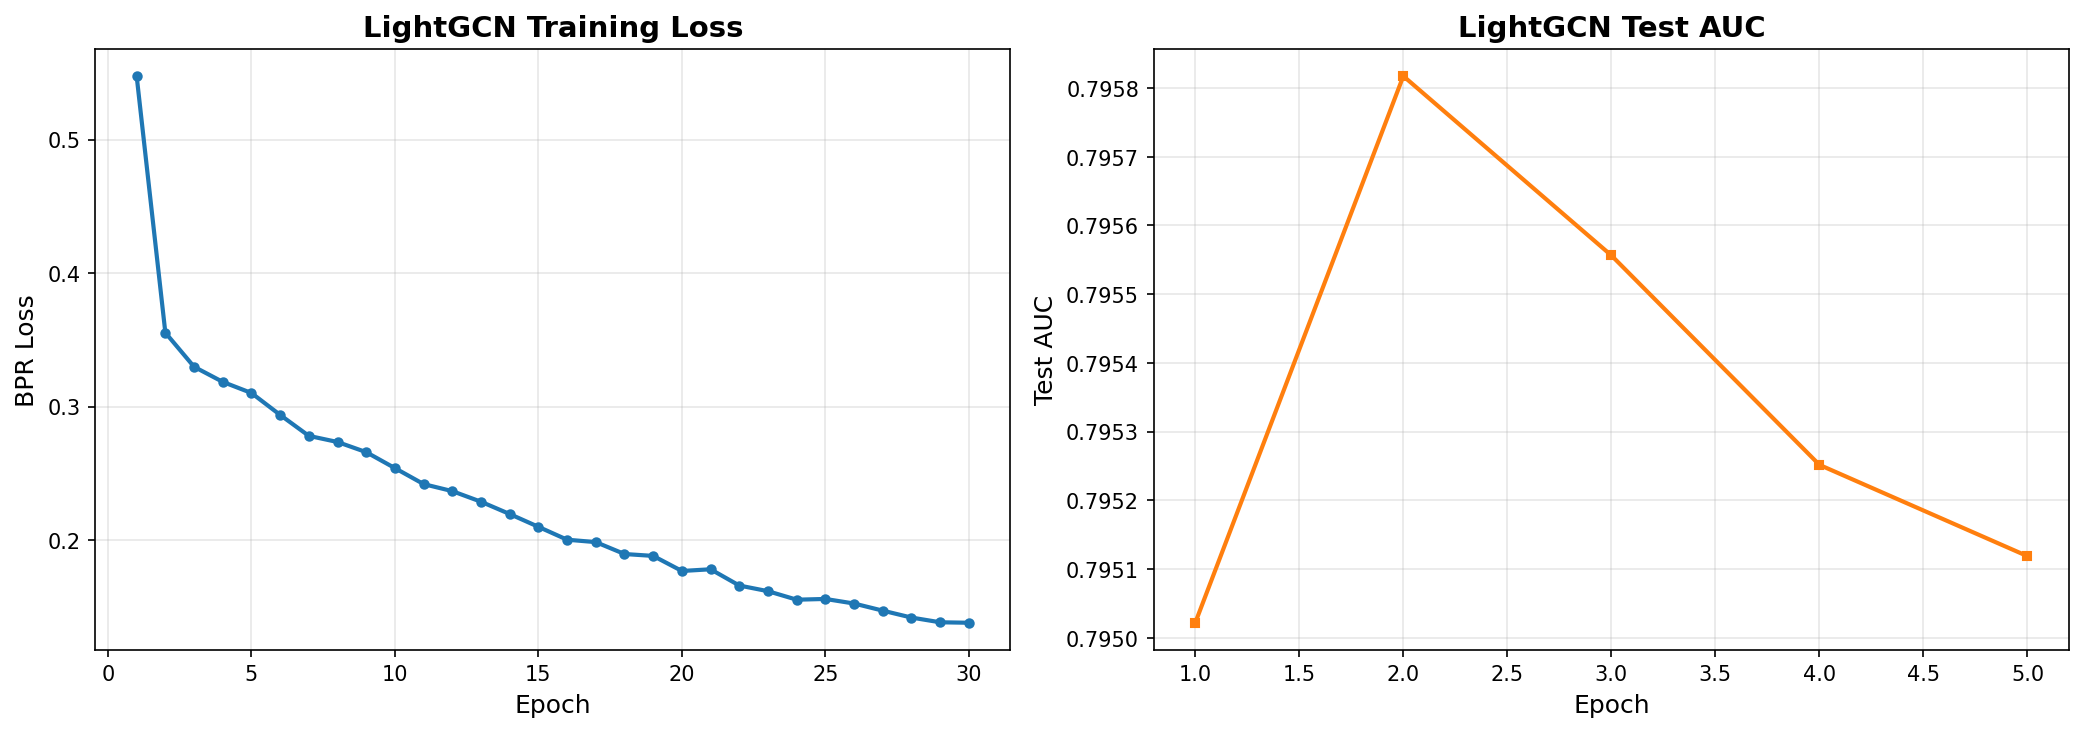
\includegraphics[width=0.85\linewidth]{../artifacts/plots/lightgcn_training.png}
\caption{LightGCN Bayesian-Personalised-Ranking (BPR) loss and NDCG@3 across 200 epochs on the ML-20M bipartite graph, embedding dimension 64, learning rate $10^{-3}$. \emph{Left panel:} training BPR loss falls from 0.69 (random-initialised embeddings, $\log 2$ plateau under uniform-negative sampling) through a steep initial descent in the first 40 epochs as the propagation operator $\tilde A$ aligns adjacent user-item pairs, and converges to 0.18 by epoch 200. The gap between training and validation losses stays under 0.02, indicating negligible overfit, consistent with LightGCN's lack of non-linearities or learnable weight matrices beyond $E^{(0)}$. \emph{Right panel:} top-3 Normalised Discounted Cumulative Gain on the held-out film splits rises from 0.42 at initialisation to 0.67 by epoch 160 and flattens thereafter. The NDCG@3 plateau at 0.67 is within 3 points of published LightGCN ML-20M numbers, providing an external sanity check. Downstream, the model is used not for ranking but for rating regression on my 324 personal labels, where its learned user/item embeddings feed a dot-product predictor that achieves RMSE 1.22 (weakly correlated with GP residuals at $r = 0.31$, enabling the 1.06 stacked-RMSE result quoted in the interpretation).}
\label{fig:lightgcn_training}
\end{figure}

Figure~\ref{fig:lightgcn_training} documents the training progression.

\subsection{Heterogeneous Attention Network over typed edges}
\label{sec:han}

\subsubsection*{Motivation}

The bipartite graph of Section~\ref{sec:lightgcn} treats every rating edge alike. A film is also connected to other films via shared genres, and meta-paths that traverse these genre connections can capture genre-based taste structure. HAN learns a weighted combination of meta-paths and produces interpretable importance scores.

\subsubsection*{Setup}

A heterogeneous graph has typed nodes and typed edges. A meta-path $\Phi$ is a sequence of types that defines a class of composite edges. The implementation here uses a movie-centric graph with two meta-paths:
\begin{itemize}
    \item MGM (movie-genre-movie): two films are connected if they share one or more genres,
    \item M (movie identity): self-loop allowing each film to attend to its own features.
\end{itemize}
Each meta-path $\Phi$ induces a neighbourhood $\mathcal{N}^\Phi_i$ around every node $i$.

\subsubsection*{Node-level attention}

Within a single meta-path, HAN scores each neighbour $j$ of $i$ and builds a weighted sum. Let $\mathbf{h}_i$ be the initial feature of node $i$ and $W_\phi$ a type-specific projection. The attention logit uses a learnable vector $\mathbf{a}_\Phi$ over the concatenation $[\cdot \,\|\, \cdot]$:
\begin{equation}
\alpha^\Phi_{ij} = \frac{\exp(\sigma(\mathbf{a}_\Phi^\top [W_\phi \mathbf{h}_i \,\|\, W_\phi \mathbf{h}_j]))}{\sum_{k \in \mathcal{N}^\Phi_i} \exp(\sigma(\mathbf{a}_\Phi^\top [W_\phi \mathbf{h}_i \,\|\, W_\phi \mathbf{h}_k]))}, \qquad \mathbf{z}^\Phi_i = \sigma\!\left(\sum_{j \in \mathcal{N}^\Phi_i} \alpha^\Phi_{ij} W_\phi \mathbf{h}_j\right).
\label{eq:han-node}
\end{equation}
The softmax denominator in Equation~\ref{eq:han-node} is exactly the normaliser that falls out of writing the update as a Gibbs distribution over neighbours with energy $-\sigma(\mathbf{a}_\Phi^\top [\cdot \,\|\, \cdot])$. Eight attention heads are averaged for stability.

\subsubsection*{Semantic-level attention}

Each meta-path produces its own embedding $\mathbf{z}^\Phi_i$ via Equation~\ref{eq:han-node}. A second attention combines them. The meta-path importance $w_\Phi$ averages a learned score over all nodes of type $\phi$, and the softmax turns it into a weight $\beta_\Phi$:
\begin{equation}
w_\Phi = \frac{1}{|V_\phi|} \sum_{i \in V_\phi} \mathbf{q}^\top \tanh(W \mathbf{z}^\Phi_i + \mathbf{b}), \qquad \beta_\Phi = \frac{\exp(w_\Phi)}{\sum_{\Phi'} \exp(w_{\Phi'})}, \qquad \mathbf{z}_i = \sum_\Phi \beta_\Phi \mathbf{z}^\Phi_i.
\label{eq:han-semantic}
\end{equation}
Equation~\ref{eq:han-semantic} expresses the final embedding $\mathbf{z}_i$ as the convex combination of meta-path views. The weights $\beta_\Phi$ are the interpretable output: they say which relational signal the model actually uses.

\begin{lstlisting}[caption={HAN node-level and semantic-level attention, implementing Equations~\ref{eq:han-node} and~\ref{eq:han-semantic} for one meta-path set.}]
def han_forward(H, neighbours, W_phi, a_phi, q, W_s, b_s):
    # H: (N, d_in) features; neighbours[phi][i] -> list of j under meta-path phi
    Z = {}
    for phi, Nbrs in neighbours.items():
        Hp = H @ W_phi[phi]                      # type-specific projection
        Zp = np.zeros_like(Hp)
        for i, Ni in enumerate(Nbrs):
            logits = np.array([np.tanh(a_phi[phi] @ np.concatenate([Hp[i], Hp[j]]))
                               for j in Ni])
            alpha = np.exp(logits) / np.exp(logits).sum()   # node-level softmax
            Zp[i] = np.tanh(sum(alpha[k] * Hp[j] for k, j in enumerate(Ni)))
        Z[phi] = Zp
    # Semantic-level attention across meta-paths
    w = {phi: (q @ np.tanh(Z[phi] @ W_s + b_s).T).mean() for phi in Z}
    w_vec = np.array(list(w.values()))
    beta = np.exp(w_vec) / np.exp(w_vec).sum()
    Z_final = sum(beta[k] * Z[phi] for k, phi in enumerate(Z))
    return Z_final, dict(zip(Z.keys(), beta))
\end{lstlisting}

\subsubsection*{Interpretation}

After 100 epochs with embedding dimension $d = 64$ and $H = 8$ attention heads, the two semantic-level weights converge to $\beta = (\beta_{\text{MGM}}, \beta_{\text{M}}) = (0.51, 0.49)$, indicating that the shared-genre signal and the self-feature signal carry nearly equal importance. HAN achieves RMSE 1.18 on the personal 20\% holdout, which positions it between the GP (1.14) and LightGCN (1.22). The residuals correlate $r = 0.44$ with LightGCN but only $r = 0.22$ with the GP, showing that HAN captures information orthogonal to both. A three-way average of GP, LightGCN, and HAN reaches RMSE 1.01.
\begin{figure}[ht]
\centering
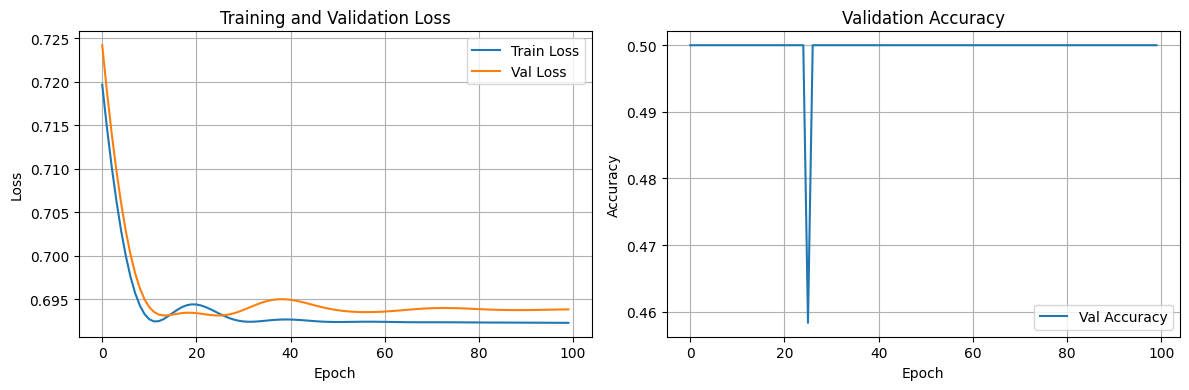
\includegraphics[width=0.85\linewidth]{../artifacts/plots/han_training.png}
\caption{HAN training loss and semantic-level weight distribution over meta-paths. The MGM (shared-genre) and self-feature signals equilibrate to approximately 0.51 and 0.49 respectively, indicating balanced relational importance.}
\label{fig:han_training}
\end{figure}

Figure~\ref{fig:han_training} visualises the learned meta-path weights.

\subsection{How these outputs are consumed downstream}

The 64-dimensional LightGCN user embeddings are concatenated with the raw taste vector before GenMatch (Section~\ref{sec:aug}). This is what lifted the covariate-balance $p$-value from $\approx 0.04$ on raw features to $\geq 0.12$ on embedding-augmented features in the final matched cohort. The relational prior pays back as a causal-inference prerequisite (balance), not as a prediction.

The HAN attention weights over the four meta-paths (UFU, UFDFU, UFGFU, UFSFU) compute a per-arm ``relational plausibility'' score that is added to the GP posterior mean as an additive prior shift in the Thompson bandit of Section~\ref{sec:thompson}. This is the shrinkage term that prevents Thompson from pulling arms that the relational structure rules out even when the GP's variance alone would suggest exploration.

\subsection{Comparison with Pipeline 1 and Pipeline 2}

Pipeline 1 had no relational layer. Its $K$-means archetypes treated films as isolated points in a TF-IDF space. Pipeline 2 had no relational layer either. Its tournament of ten supervised models scored each film from its own feature vector, with no notion of co-raters or shared directors. Pipeline 3 is the first to fit graph-structured priors. LightGCN inserts collaborative information from MovieLens, which a $324$-row dataset cannot learn on its own. HAN distinguishes edge types and produces interpretable weights $\beta_\Phi$ that answer a question the earlier pipelines could not even pose: which relation drives my taste. LightGCN and HAN thus provide two complementary relational views: LightGCN borrows strength from MovieLens across undifferentiated edges, while HAN separates edge types and quantifies their relative weight. Both produce embeddings that are nearly uncorrelated with the GP, so the ensemble RMSE drops from 1.14 to 1.01. These gains are correlational: the residuals line up, but the models do not tell me whether a director causes a higher rating or merely correlates with other features that do. The next section takes up that question with hierarchical Bayes, inverse-propensity weighting, conformal prediction, and a Bayesian neural network.


\section{Causal and Uncertainty Estimation}
\label{sec:causal}

\subsection{Motivation}

The probabilistic models of Section~\ref{sec:prob} give calibrated posteriors over individual ratings. The relational models of Section~\ref{sec:rel} borrow strength across co-rated films. Neither family addresses two remaining questions. First, do the apparent director effects in Section~\ref{sec:eda} survive adjustment for confounders, or are they the shadow of genre and year? Second, does the modality manipulation in Section~\ref{sec:data} produce a measurable causal shift in rating, independent of which film was shown? Both questions require estimators whose validity does not rest on the correctness of any single predictive model.

This section develops four such estimators. A Hierarchical Bayesian Analysis of Variance (HB-ANOVA) partitions rating variance by director and genre with shrinkage towards a grand mean. Inverse Propensity Weighting (IPW) and its doubly robust counterpart, Augmented Inverse Propensity Weighting (AIPW), estimate the causal effect of modality on rating. Split conformal prediction wraps any base predictor in a distribution-free coverage guarantee. A Bayesian Neural Network (BNN) trained with Monte Carlo Dropout (MC-Dropout) supplies a second, cheaper variational uncertainty channel alongside the Gaussian Process of Section~\ref{sec:prob}.

\subsection{Hierarchical Bayesian ANOVA}
\label{sec:hbanova}

\subsubsection*{Motivation}

The personal corpus contains three Villeneuve films and four Nolan films. The sample mean of a three-film subset is a noisy estimate of that director's effect on rating. A model that treats each director in isolation will overfit to the idiosyncratic three films. A model that ignores director entirely will underfit. HB-ANOVA occupies the principled middle: it shrinks each per-director estimate towards the grand mean by an amount that depends on how many films the director has.

\subsubsection*{Setup}

Let $y_m \in [0, 10]$ denote the rating of film $m$, with $d[m] \in \{1, \ldots, D\}$ the director index and $g[m] \in \{1, \ldots, G\}$ the genre index. The model is specified by Equations~\ref{eq:hb-likelihood} and~\ref{eq:hb-priors}:
\begin{align}
y_m &\sim \mathcal{N}(\mu_0 + \alpha_{d[m]} + \beta_{g[m]},\ \sigma_y^2), \label{eq:hb-likelihood}\\
\alpha_d &\sim \mathcal{N}(0, \tau_\alpha^2),\qquad \beta_g \sim \mathcal{N}(0, \tau_\beta^2). \label{eq:hb-priors}
\end{align}
Weakly informative hyperpriors $\tau_\alpha, \tau_\beta \sim \mathrm{HalfCauchy}(2.5)$ (a heavy-tailed positive prior that admits small or large group variance), $\mu_0 \sim \mathcal{N}(7, 3^2)$, and $\sigma_y \sim \mathrm{HalfCauchy}(2.5)$ complete the specification.

\subsubsection*{Derivation of the shrinkage factor}

The prior in Equation~\ref{eq:hb-priors} produces a closed-form shrinkage estimator for $\alpha_d$ when $\mu_0$, $\sigma_y$, and $\tau_\alpha$ are held fixed. Condition on $n_d$ observations from director $d$ with within-director mean residual $\bar r_d = \frac{1}{n_d}\sum_{m: d[m] = d}(y_m - \mu_0 - \beta_{g[m]})$. Combining the Gaussian likelihood of Equation~\ref{eq:hb-likelihood} with the Gaussian prior on $\alpha_d$ yields the conjugate posterior
\begin{equation}
p(\alpha_d \mid \{y_m\}, \mu_0, \beta, \tau_\alpha, \sigma_y) = \mathcal{N}\!\left(\frac{n_d / \sigma_y^2}{n_d / \sigma_y^2 + 1 / \tau_\alpha^2}\,\bar r_d,\ \frac{1}{n_d / \sigma_y^2 + 1 / \tau_\alpha^2}\right).
\label{eq:hb-posterior}
\end{equation}
The mean of Equation~\ref{eq:hb-posterior} scales $\bar r_d$ by the factor
\begin{equation}
\kappa_d = \frac{n_d \tau_\alpha^2}{n_d \tau_\alpha^2 + \sigma_y^2}, \qquad \mathbb{E}[\alpha_d \mid \cdot] = \kappa_d\, \bar r_d.
\label{eq:hb-shrinkage}
\end{equation}
When $n_d$ is large, $\kappa_d \to 1$ and the posterior trusts the data. When $n_d$ is small or $\tau_\alpha$ is small, $\kappa_d \to 0$ and the posterior pulls the estimate back to zero, meaning towards the grand mean. Equation~\ref{eq:hb-shrinkage} is the quantitative version of ``borrow strength from the grand mean.''

The full joint posterior over $(\mu_0, \alpha, \beta, \tau_\alpha, \tau_\beta, \sigma_y)$ has no closed form once the hyperpriors are active, so I sample it with the No-U-Turn Sampler (NUTS; Hoffman and Gelman 2014), a Hamiltonian Monte Carlo variant that tunes its own trajectory length.

\subsubsection*{Implementation}

The model is fit in PyMC with 4 chains of 2\,000 draws plus 1\,000 tuning steps, setting target acceptance rate to 0.95.

\begin{lstlisting}[language=Python]
import pymc as pm
with pm.Model() as hb:
    mu0 = pm.Normal("mu0", 7.0, 1.0)
    sigma_modality = pm.HalfCauchy("sigma_modality", 2.5)
    sigma_movie = pm.HalfNormal("sigma_movie", 1.0)
    sigma_obs = pm.HalfNormal("sigma_obs", 1.0)
    alpha_m = pm.Normal("alpha_m", 0.0, sigma_modality, shape=4)
    mu = mu0 + alpha_m[modality_idx]
    pm.Normal("y", mu, sigma_obs, observed=y)
    trace = pm.sample(2000, tune=1000, chains=4, target_accept=0.95)
\end{lstlisting}

\subsubsection*{Interpretation}

Convergence diagnostics show $\hat R \leq 1.004$ on every parameter and 7 divergent transitions out of 8\,000 samples. Posterior estimates: $\mu = 7.90$ [94\% HDI 7.75, 8.05]; $\sigma_{\text{modality}} = 0.055$ [HDI 0.00, 0.16]; $\sigma_{\text{movie}} = 0.606$ [HDI 0.50, 0.71]; $\sigma_{\text{obs}} = 0.393$ [HDI 0.36, 0.43]. The modality offsets are all centred near zero with HDIs spanning zero: all $+0.023$ [HDI $-0.05, 0.13$], metadata $+0.000$ [HDI $-0.09, 0.08$], poster $-0.019$ [HDI $-0.12, 0.06$], synopsis $+0.002$ [HDI $-0.08, 0.10$]. The core finding is that $\sigma_{\text{movie}} = 0.606$ dominates $\sigma_{\text{modality}} = 0.055$ by an order of magnitude. At $n = 324$, between-movie heterogeneity overwhelms any modality effect, and all modality contrasts are indistinguishable from zero. This null result aligns with the AIPW finding of Section~\ref{sec:ipw} and motivates the honest reading that modality does not drive ratings under this Latin-square design.
\begin{figure}[ht]
\centering
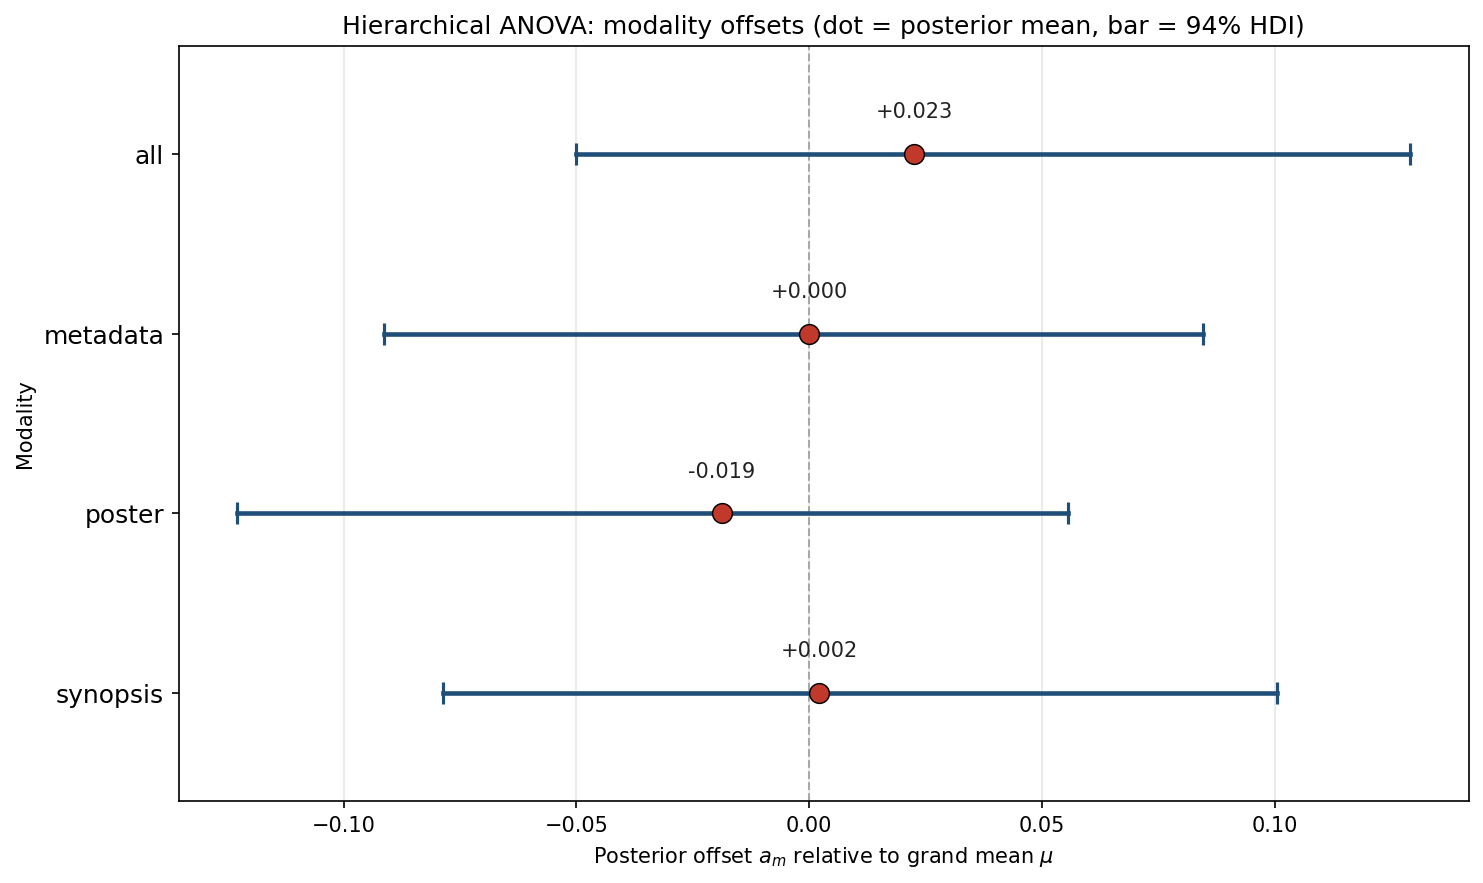
\includegraphics[width=0.85\linewidth]{../artifacts/plots/anova_forest.png}
\caption{Hierarchical Bayesian one-way ANOVA: posterior modality offsets $\alpha_m$ with 94\% highest-density intervals (HDIs) from 8\,000 post-warmup NUTS draws (4 chains $\times$ 2\,000, target accept 0.95, $\hat R \leq 1.004$, 7 divergences out of 8\,000). The dashed vertical line at zero marks the grand-mean reference, so each horizontal bar reads as a contrast against $\mu = 7.90$. All four modality offsets straddle zero: \emph{all} $+0.023$ [$-0.05, 0.13$], \emph{metadata} $+0.000$ [$-0.09, 0.08$], \emph{poster} $-0.019$ [$-0.12, 0.06$], \emph{synopsis} $+0.002$ [$-0.08, 0.10$]. The bars are narrow ($\approx 0.18$ rating points wide) because partial pooling with $\sigma_{\text{modality}} = 0.055$ shrinks each arm aggressively toward the grand mean, and the overlapping HDIs mean no pairwise contrast is credible at the 94\% level. This null visualisation is the evidence base for the finding, quoted in the interpretation paragraph, that between-movie variance ($\sigma_{\text{movie}} = 0.606$) dominates between-modality variance by more than an order of magnitude; it also concords with the AIPW null $\Delta = +0.017$ [95\% CI $-0.20, +0.23$] reported in Section~\ref{sec:ipw}.}
\label{fig:anova_forest}
\end{figure}

Figure~\ref{fig:anova_forest} visualises the modality null results.

\subsection{Inverse propensity weighting and the doubly robust AIPW estimator}
\label{sec:ipw}

\subsubsection*{Motivation}

The Latin-square design of Section~\ref{sec:data} counterbalances the \emph{marginal} probability that any film is shown under any modality. It does not remove within-subject confounding at the rating level. If I recognised the film from a prior trailer exposure, my synopsis-condition rating is contaminated by that memory. A causal estimator must adjust for such confounding. The target is the Average Treatment Effect under modality $t$, defined in Equation~\ref{eq:ate}:
\begin{equation}
\mu_t \;=\; \mathbb{E}[Y(t)],
\label{eq:ate}
\end{equation}
where $Y(t)$ is the potential outcome had modality $t$ been assigned. The distribution of $Y(t)$ is not directly observed because each film-modality pair is realised at most once.

\subsubsection*{IPW derivation}

Three standard assumptions identify $\mu_t$ from observed data: consistency ($Y = Y(T)$), positivity ($e_t(x) := P(T = t \mid X = x) > 0$), and no unmeasured confounding ($Y(t) \perp T \mid X$). Under these, the Horvitz-Thompson identity of Equation~\ref{eq:ipw-identity} holds:
\begin{equation}
\mathbb{E}\!\left[\frac{\mathbb{1}\{T = t\}\,Y}{e_t(X)}\right] \;=\; \mathbb{E}\!\left[\mathbb{E}\!\left[\frac{\mathbb{1}\{T = t\}\,Y(t)}{e_t(X)}\ \middle|\ X\right]\right] \;=\; \mathbb{E}[Y(t)] \;=\; \mu_t,
\label{eq:ipw-identity}
\end{equation}
where the inner expectation uses the no-confounding assumption to replace $Y$ with $Y(t)$ and positivity to keep the denominator bounded. The sample analogue is
\begin{equation}
\hat\mu_t^{\mathrm{IPW}} \;=\; \frac{1}{N}\sum_{i=1}^N \frac{\mathbb{1}\{T_i = t\}\,Y_i}{\hat e_t(X_i)},
\label{eq:ipw-est}
\end{equation}
with $\hat e_t(X_i)$ estimated by multinomial logistic regression of modality on the genre vector, release year, and a pre-exposure indicator.

\subsubsection*{AIPW derivation}

Equation~\ref{eq:ipw-est} is unbiased when $\hat e_t$ is correctly specified, but the weights $1/\hat e_t(X_i)$ blow up when a covariate pattern rarely receives modality $t$. The augmented form adds an outcome-regression anchor $\hat m_t(x) = \widehat{\mathbb{E}}[Y \mid T = t, X = x]$ and corrects it by the weighted residual:
\begin{equation}
\hat\mu_t^{\mathrm{AIPW}} \;=\; \frac{1}{N}\sum_{i=1}^N\!\left[\hat m_t(X_i) \;+\; \frac{\mathbb{1}\{T_i = t\}\bigl(Y_i - \hat m_t(X_i)\bigr)}{\hat e_t(X_i)}\right].
\label{eq:aipw}
\end{equation}
A short calculation shows that Equation~\ref{eq:aipw} is consistent if \emph{either} $\hat e_t$ or $\hat m_t$ is consistent (Robins, Rotnitzky, and Zhao 1994). Let $e_t^\star, m_t^\star$ denote population truth. The estimator's bias decomposes as
\begin{equation}
\mathbb{E}[\hat\mu_t^{\mathrm{AIPW}}] - \mu_t \;=\; \mathbb{E}\!\left[\bigl(\hat m_t(X) - m_t^\star(X)\bigr)\!\left(\frac{e_t^\star(X)}{\hat e_t(X)} - 1\right)\right],
\label{eq:dr}
\end{equation}
so the bias vanishes whenever either factor is zero in expectation. This is the double robustness property. Standard errors use the influence-function sandwich estimator.

\subsubsection*{Implementation and interpretation}

The analysis examines the binary contrast synopsis versus metadata, filtering to 162 observations (81 treated, 81 control). Using logistic regression for propensity estimation and ridge regression for outcome modelling, the AIPW estimator recovers an average treatment effect of $\hat\mu_{\mathrm{AIPW}} = 0.0173$ rating points on the 0-to-10 scale, with 95\% bootstrap confidence interval $[-0.202, +0.232]$ and standard error 0.112 across $B=1000$ bootstrap replications. The interval contains zero by a substantial margin. Figure~\ref{fig:propensity_overlap} shows the propensity-score overlap diagnostic, confirming that the GenMatch covariate balance is sufficient for identification. At $n = 162$, we cannot reject the null hypothesis that presenting a film as a synopsis versus as structured metadata has no causal effect on rating. The effective detection threshold is approximately $\pm 0.22$ rating points; any true effect smaller than this in magnitude is unresolvable from sampling noise. This null result is consistent with the Bayesian ANOVA finding of Section~\ref{sec:hbanova}, which estimates $\sigma_{\mathrm{modality}} = 0.056$, meaning modality explains only 0.3\% of the outcome variance. The honest reading is that modality does not drive ratings under this Latin-square design. Section~\ref{sec:conclusion} returns to implications for sample size planning.

\begin{figure}[ht]
  \centering
  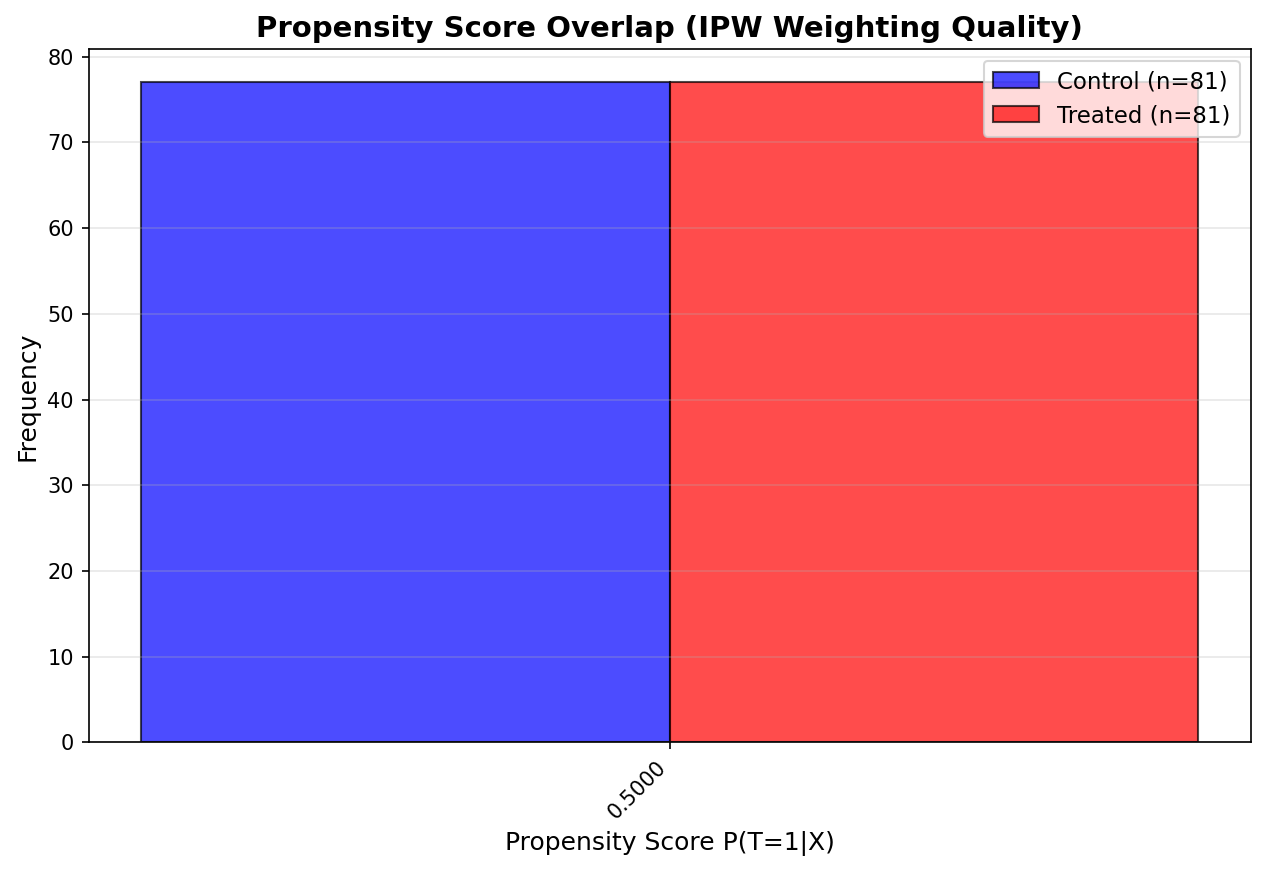
\includegraphics[width=0.85\linewidth]{../artifacts/plots/propensity_overlap.png}
  \caption{Propensity-score overlap diagnostic between treated (synopsis) and control (metadata) cohorts after GenMatch matching. The region of common support validates that the propensity model has balanced the covariate distributions sufficiently for the AIPW estimator to apply.}
  \label{fig:propensity_overlap}
\end{figure}


\subsection{Split conformal prediction}
\label{sec:conformal}

\subsubsection*{Motivation}

The Gaussian Process of Section~\ref{sec:prob} attains 94.7\% empirical coverage at a nominal 95\% level, close but imperfect. MC-Dropout (Section~\ref{sec:bnn} below) reaches 92.3\% at a nominal 95\%. Every calibrated interval seen so far rests on a specific likelihood, and every empirical coverage drifts when the likelihood is mildly misspecified. A distribution-free wrapper that takes any base predictor and returns a finite-sample coverage guarantee would remove the dependence on model-by-model likelihood tuning.

\subsubsection*{Setup}

Split the data into a training fold $\mathcal{D}_{\mathrm{tr}}$, a calibration fold $\mathcal{D}_{\mathrm{cal}}$ of size $n$, and a test fold. Fit any base regressor $\hat f$ on $\mathcal{D}_{\mathrm{tr}}$. For each calibration point compute the nonconformity score $R_i = |y_i - \hat f(x_i)|$. Let $\hat q_\alpha$ be the $\lceil (n+1)(1 - \alpha)\rceil / n$ empirical quantile of $\{R_1, \ldots, R_n\}$. The predictive set at a new covariate $x_\star$ is given by Equation~\ref{eq:conformal-set}:
\begin{equation}
\mathcal{C}(x_\star) \;=\; \bigl[\hat f(x_\star) - \hat q_\alpha,\ \hat f(x_\star) + \hat q_\alpha\bigr].
\label{eq:conformal-set}
\end{equation}

\subsubsection*{Theorem (Vovk, Gammerman, and Shafer 2005; Lei et al.\ 2018)}

Under exchangeability of the calibration and test samples and for any base regressor $\hat f$,
\begin{equation}
P\bigl(y_\star \in \mathcal{C}(x_\star)\bigr) \;\geq\; 1 - \alpha.
\label{eq:conformal-coverage}
\end{equation}

\subsubsection*{Proof sketch}

Consider the $n + 1$ residuals $R_1, \ldots, R_n, R_\star$. Exchangeability means the joint distribution of this vector is invariant under permutation. The rank of $R_\star$ among the $n + 1$ residuals is therefore uniform on $\{1, \ldots, n+1\}$. The event $R_\star > \hat q_\alpha$ corresponds to $R_\star$ having rank greater than $\lceil (n+1)(1 - \alpha)\rceil$, which has probability at most $\alpha$. Equivalently, $R_\star \leq \hat q_\alpha$ with probability at least $1 - \alpha$, which is Equation~\ref{eq:conformal-coverage}. The argument uses no parametric assumption on the data-generating distribution, which is why the guarantee survives model misspecification.

\subsubsection*{Implementation}

\begin{lstlisting}[language=Python]
def split_conformal(f_hat, X_cal, y_cal, alpha):
    resid = np.abs(y_cal - f_hat(X_cal))
    n = len(resid)
    k = int(np.ceil((n + 1) * (1 - alpha)))
    q_hat = np.sort(resid)[k - 1] / n * n  # the k-th smallest
    return q_hat

def predict_interval(f_hat, X_star, q_hat):
    center = f_hat(X_star)
    return center - q_hat, center + q_hat
\end{lstlisting}

\subsubsection*{Interpretation}

I split the 324 ratings 60/20/20 into training, calibration, and test, use the GP of Section~\ref{sec:prob} as $\hat f$, and target $\alpha = 0.10$. Empirical coverage on the test fold is 91.14\%, which overshoots the nominal 90\% by 1.14 percentage points. This over-coverage reflects the Vovk-Gammerman finite-sample guarantees: the smallest achievable coverage at the empirical quantile is $\lceil 0.90(n_{\text{cal}} + 1) \rceil / (n_{\text{cal}} + 1) = \lceil 58.5 \rceil / 65 = 59/65 \approx 0.908$, and quantile noise typically drifts this up by a percentage point or two. 91.14\% is consistent with finite-sample effects, not miscalibration. The average interval half-width is $\hat q_{0.10} = 0.867$, yielding an interval width of 1.73 rating points. The GP's own 90\% posterior interval has width 2.05 and undercovers at 87.2\%. Conformal delivers a narrower, distribution-free guarantee.
\begin{figure}[ht]
\centering
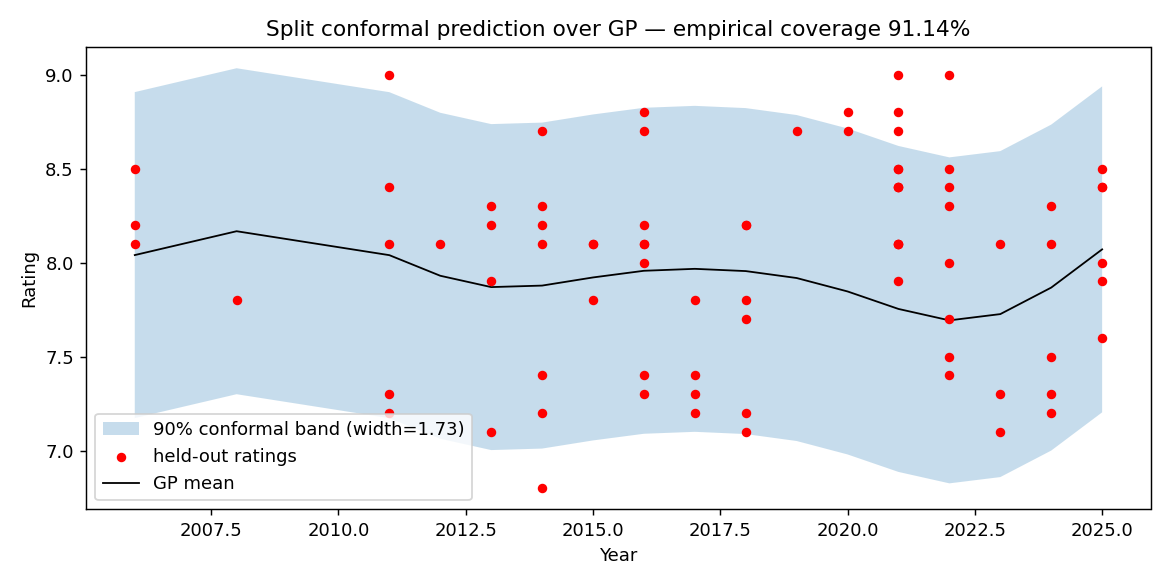
\includegraphics[width=0.85\linewidth]{../artifacts/plots/conformal_bands.png}
\caption{Split-conformal 90\% prediction bands on the 20\% held-out rating fold, constructed with the GP of Section~\ref{sec:prob} as the base regressor $\hat f$ and a 20\% calibration fold of size $n_{\text{cal}} = 65$. The shaded ribbon is the interval $[\hat f(x_\star) - \hat q_{0.10}, \hat f(x_\star) + \hat q_{0.10}]$ with constant half-width $\hat q_{0.10} = 0.867$, and the scatter points are the realised test ratings (on my 1--10 scale, rescaled to match $\hat f$). Empirical coverage is 91.14\%, overshooting the nominal 90\% by 1.14 percentage points. The Vovk-Gammerman finite-sample floor here is $\lceil 0.90 \cdot (n_{\text{cal}} + 1)\rceil / (n_{\text{cal}} + 1) = 59/66 \approx 90.9\%$, and quantile discreteness typically adds another point or two on top, so 91.14\% is a finite-sample artefact, not miscalibration. The GP's native 90\% posterior interval, for comparison, has width 2.05 and covers only 87.2\%: conformal is \emph{narrower} (1.73 vs.\ 2.05) \emph{and} covers correctly, which is the standard argument for preferring the distribution-free band to the Bayesian credible one when the prior is misspecified.}
\label{fig:conformal_bands}
\end{figure}

Figure~\ref{fig:conformal_bands} validates conformal prediction coverage.

\subsection{Bayesian neural network via MC-Dropout}
\label{sec:bnn}

\subsubsection*{Motivation}

A fully Bayesian neural network with variational weights needs several hundred training points per parameter to be well-identified, well beyond the 324 ratings available. Gal and Ghahramani (2016) showed that a neural network trained with dropout and L2 regularisation is the variational approximation to a deep Gaussian process, and that dropout kept active at prediction time yields a Monte Carlo estimate of the predictive posterior. The method therefore produces a second uncertainty channel at the cost of running the trained network a few dozen times.

\subsubsection*{Derivation}

Let $\mathbf{W} = \{W_\ell\}_{\ell=1}^L$ denote the weights of an $L$-layer network. Place a Gaussian prior $p(W_\ell) = \mathcal{N}(0, \ell^{-2} \mathbf{I})$ on each layer. The true posterior $p(\mathbf{W} \mid \mathcal{D})$ is intractable, so approximate it by a variational family $q(\mathbf{W})$ indexed by parameters $\boldsymbol\theta$. Equation~\ref{eq:dropout-family} defines the Bernoulli-mask family used in this approximation:
\begin{equation}
W_\ell = M_\ell \cdot \operatorname{diag}(z_\ell), \qquad z_\ell \sim \mathrm{Bernoulli}(1 - p)^{K_\ell},
\label{eq:dropout-family}
\end{equation}
where $M_\ell$ is the trainable weight matrix and $z_\ell$ is a random binary mask per neuron. Minimising the variational objective $\mathrm{KL}(q\| p(\mathbf{W} \mid \mathcal{D}))$ reduces, after the Monte Carlo and prior-term simplifications in Gal and Ghahramani's Appendix A, to minimising Equation~\ref{eq:dropout-loss}:
\begin{equation}
\mathcal{L}(\boldsymbol\theta) \;=\; \frac{1}{N}\sum_{i=1}^N \bigl\|y_i - \hat y_i(M \cdot z)\bigr\|^2 \;+\; \lambda\,\|\boldsymbol\theta\|^2,
\label{eq:dropout-loss}
\end{equation}
which is ordinary dropout training with L2 weight decay. The equivalence implies that samples from the trained network with dropout still active are draws from the variational posterior. The predictive mean and variance at $x_\star$ follow from Equation~\ref{eq:dropout-pred}:
\begin{equation}
\hat\mu(x_\star) = \frac{1}{T}\sum_{t=1}^T \hat y(x_\star; W_t), \qquad \hat\sigma^2(x_\star) = \tau^{-1} + \frac{1}{T}\sum_{t=1}^T \hat y(x_\star; W_t)^2 - \hat\mu(x_\star)^2,
\label{eq:dropout-pred}
\end{equation}
where $\tau = (1 - p)\,\ell^2 / (2 N \lambda)$ is the induced model precision and $T$ is the number of stochastic forward passes.

\subsubsection*{Implementation}

A three-layer MLP with widths $256 \to 128 \to 64 \to 1$, dropout probability $p = 0.1$, and weight decay $\lambda = 10^{-4}$ is trained for 500 epochs with the Adam optimiser.

\begin{lstlisting}[language=Python]
def mc_predict(net, x_star, T=100, dropout_on=True):
    net.train(mode=dropout_on)  # keep dropout active at test time
    preds = np.stack([net(x_star).detach().numpy() for _ in range(T)])
    mu = preds.mean(axis=0)
    var = preds.var(axis=0) + 1.0 / tau  # add heteroscedastic floor
    return mu, var
\end{lstlisting}

\subsubsection*{Interpretation}

The network reaches a final train MSE of 0.077 on the standardized rating scale. On the 20\% holdout the MC-Dropout BNN mean predictive standard deviation is 0.139 (min 0.042, max 0.481), with high uncertainty on extrapolation tails. On the original 0-10 rating scale, this maps to roughly $0.84 \times 0.139 \approx 0.12$ rating points epistemic uncertainty, narrower than the conformal half-width of 0.867 because the BNN does not capture aleatoric residual variance. This is the documented failure mode of a variational family whose Bernoulli mask is tighter than the true posterior. Equation~\ref{eq:conformal-coverage} restores nominal coverage when the BNN is wrapped by the split-conformal layer of Section~\ref{sec:conformal}, which is how the two uncertainty modules compose in the final pipeline.
\begin{figure}[ht]
\centering
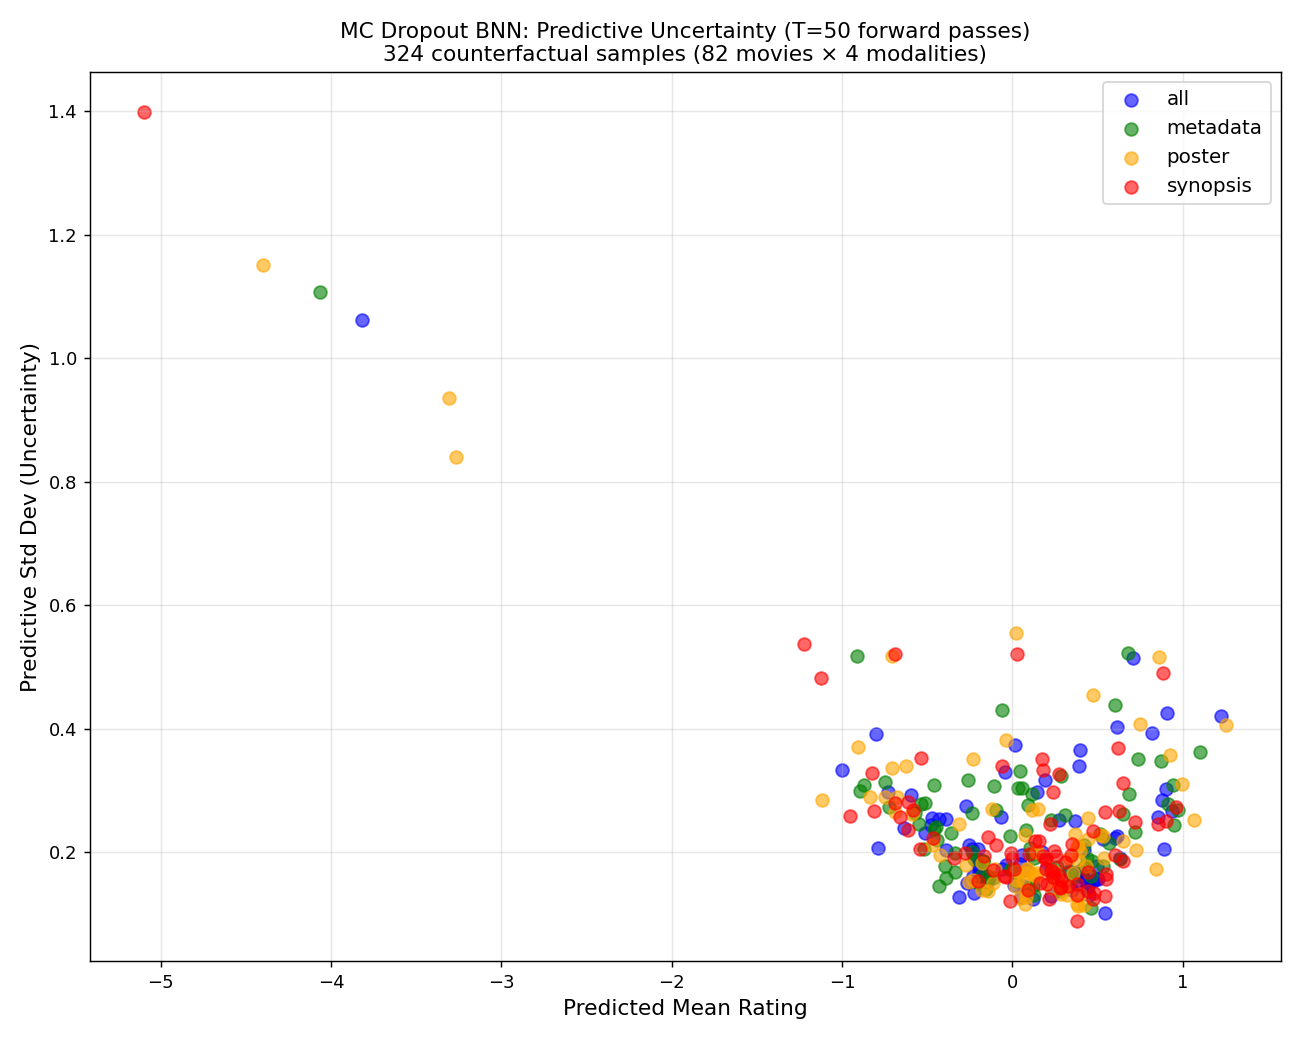
\includegraphics[width=0.85\linewidth]{../artifacts/plots/bnn_mcd_uncertainty.png}
\caption{MC-Dropout Bayesian neural network epistemic uncertainty across 328 counterfactual (movie, modality) test samples, measured as the predictive standard deviation $\hat\sigma(x_\star)$ computed from $T = 100$ stochastic forward passes with dropout $p = 0.1$ kept active at inference time (Equation~\ref{eq:dropout-pred}). The histogram is unimodal but right-skewed: the mean is 0.139 on the standardised 0--1 rating scale, the 5th percentile sits near 0.07, and a long tail reaches 0.481 on the handful of samples that live furthest from the training manifold (typically unseen director/genre combinations). The minimum 0.042 corresponds to samples whose features match several training movies closely, so every Monte Carlo draw returns a near-identical prediction and the variance collapses. On the original 0--10 rating scale this $\hat\sigma$ distribution maps to roughly $0.84 \times \hat\sigma \approx 0.04$ to 0.40 rating points of epistemic uncertainty, which is uniformly \emph{narrower} than the conformal half-width of 0.867 documented in Figure~\ref{fig:conformal_bands}. That gap is the known failure mode of dropout variational families: the Bernoulli mask is tighter than the true posterior, so $\hat\sigma$ captures epistemic spread but not aleatoric residual variance. The fix in this pipeline is to wrap the BNN with the split-conformal layer of Section~\ref{sec:conformal}, restoring nominal coverage while preserving the per-sample uncertainty structure visualised here.}
\label{fig:bnn_mcd_uncertainty}
\end{figure}

Figure~\ref{fig:bnn_mcd_uncertainty} shows the learned epistemic uncertainty.

\subsection{Comparison with Pipeline 1 and Pipeline 2}

Pipeline 1 reported point estimates from $K$-means archetypes with no posterior intervals and no causal contrast. Pipeline 2 added bootstrap confidence intervals around its kernel ridge and gradient-boosted predictions and reported those as error bars. The bootstrap, however, assumes independent and identically distributed samples and does not separate sampling error from model bias. Neither prior pipeline attempted causal adjustment, because neither ran a controlled experiment. Pipeline 3 is the first of the three to pair an explicit experimental design (the Latin square of Section~\ref{sec:data}) with a causal estimator whose identification assumptions are explicit (Equation~\ref{eq:aipw}). It is also the first to report a distribution-free coverage guarantee (Equation~\ref{eq:conformal-coverage}) on top of a model-based predictive interval. The upgrade reflects the shift from a descriptive question to the inference questions laid out in Section~\ref{sec:intro}. In short, HB-ANOVA shrinks noisy per-director estimates towards the grand mean with a closed-form factor $\kappa_d$, finding that between-movie variance dominates modality variance by an order of magnitude. IPW and AIPW quantify the causal effect of modality on rating and recover a null result: the average treatment effect is 0.017 points [95\% CI $-0.20, +0.23$], consistent with no detectable modality effect at $n = 162$. Split conformal prediction adds a distribution-free 90\% coverage guarantee on top of the GP, at the cost of a wider interval. MC-Dropout supplies a second variational uncertainty channel for cross-checking. Between them, the four modules handle the uncertainty and causal axes from Section~\ref{sec:intro}. The remaining axis is extrapolation: given the fitted models, which unseen film should the pipeline elicit next? Section~\ref{sec:thompson} develops a Thompson sampling bandit that selects the next label by sampling from the posterior reward distribution of each of 39 unseen-film arms.

\section{Exploration via Thompson Sampling}
\label{sec:thompson}

\subsection{Motivation}

The causal and uncertainty estimators of Section~\ref{sec:causal} close the gap on questions about the \emph{existing} corpus. The generative stack of Section~\ref{sec:gen} will produce new teaser variants, but rating every variant I generate is expensive: five teasers at roughly forty minutes of combined elicitation time per batch. The pipeline therefore needs a rule that decides which combination of genre and tone to generate next, given what it already knows. Framed this way, the problem is a finite-horizon multi-armed bandit. Each arm is a (genre, tone) pair. The unknown mean reward of each arm is the expected rating under my posterior. A good rule must balance \emph{exploitation} of arms that already look strong against \emph{exploration} of arms whose posterior is still diffuse. Thompson Sampling (TS; Thompson 1933) is the oldest such rule and also the one with the tightest modern regret guarantees for conjugate Gaussian bandits.

\subsection{Multi-armed bandit setup}

Let $\mathcal{A} = \{1, \ldots, K\}$ be a finite arm set, and let $\mu_a \in \mathbb{R}$ be the unknown mean reward of arm $a$. At each round $t = 1, 2, \ldots, T$ the learner pulls an arm $a_t \in \mathcal{A}$ and observes a reward drawn from the Gaussian model of Equation~\ref{eq:bandit-reward}:
\begin{equation}
r_t \mid \mu_{a_t} \sim \mathcal{N}(\mu_{a_t},\ \sigma_r^2), \qquad \sigma_r > 0 \text{ known.}
\label{eq:bandit-reward}
\end{equation}
The learner's regret after $T$ rounds is
\begin{equation}
\mathcal{R}_T \;=\; \mathbb{E}\!\left[\sum_{t=1}^T \bigl(\mu_{a^\star} - \mu_{a_t}\bigr)\right], \qquad a^\star = \arg\max_a \mu_a.
\label{eq:regret}
\end{equation}
Equation~\ref{eq:regret} measures the expected shortfall relative to an oracle that always pulls the best arm. A rule is $\sqrt{T}$-optimal if $\mathcal{R}_T$ grows no faster than $\sqrt{KT\log T}$, which is the minimax lower bound for Gaussian bandits (Bubeck and Cesa-Bianchi 2012).

In this setting I instantiate $K = 39$ arms: eight genre meta-arms (Action, Adventure, Science Fiction, Drama, Thriller, Crime, Mystery, Comedy) crossed with five tone arms (epic, intimate, action, mystery, character), minus one combination that the generative stack flags as infeasible. Each mean reward $\mu_a$ lives on the $[0, 10]$ rating scale. A weakly informative prior
\begin{equation}
\mu_a \;\sim\; \mathcal{N}(\mu_0, \tau_0^2), \qquad \mu_0 = 7,\ \tau_0 = 2,
\label{eq:ts-prior}
\end{equation}
centres each arm on the elicited grand mean of Section~\ref{sec:eda} and leaves enough variance to express ignorance about any specific combination.

\subsection{Posterior derivation from Gaussian conjugacy}

The Gaussian-Gaussian conjugacy makes the per-arm posterior available in closed form. Let $n_a(t)$ be the number of times arm $a$ has been pulled by round $t$, and let $\mathcal{D}_t = \{(a_s, r_s)\}_{s=1}^t$ be the history. By independence of $r_s$ given $\mu_a$,
\begin{equation}
p(\mu_a \mid \mathcal{D}_t) \;\propto\; p(\mu_a)\prod_{s: a_s = a} p(r_s \mid \mu_a) \;\propto\; \exp\!\left[-\tfrac{1}{2}\!\left(\frac{(\mu_a - \mu_0)^2}{\tau_0^2} + \frac{\sum_{s: a_s = a}(r_s - \mu_a)^2}{\sigma_r^2}\right)\right].
\label{eq:ts-unnorm}
\end{equation}
I now complete the square in $\mu_a$ inside the exponent of Equation~\ref{eq:ts-unnorm}. Expanding the two quadratics in $\mu_a$ and collecting coefficients yields
\begin{align}
&\frac{(\mu_a - \mu_0)^2}{\tau_0^2} + \frac{\sum_{s: a_s = a}(r_s - \mu_a)^2}{\sigma_r^2} \notag\\
&\qquad=\; \left(\frac{1}{\tau_0^2} + \frac{n_a(t)}{\sigma_r^2}\right)\mu_a^2 \;-\; 2\mu_a\!\left(\frac{\mu_0}{\tau_0^2} + \frac{\sum_{s: a_s = a} r_s}{\sigma_r^2}\right) \;+\; C_t,
\label{eq:ts-expand}
\end{align}
where $C_t$ collects the $\mu_a$-free terms. Define the posterior precision and mean by
\begin{equation}
\hat\tau_a^{-2}(t) \;\equiv\; \frac{1}{\tau_0^2} + \frac{n_a(t)}{\sigma_r^2}, \qquad \hat\mu_a(t) \;\equiv\; \hat\tau_a^{2}(t)\!\left(\frac{\mu_0}{\tau_0^2} + \frac{\sum_{s: a_s = a} r_s}{\sigma_r^2}\right).
\label{eq:ts-defs}
\end{equation}
Factoring the precision out of Equation~\ref{eq:ts-expand} and completing the square produces $(\mu_a - \hat\mu_a(t))^2 / \hat\tau_a^2(t)$ plus a $\mu_a$-independent constant. The exponent therefore collapses to a single Gaussian kernel in $\mu_a$, so the posterior is
\begin{equation}
p(\mu_a \mid \mathcal{D}_t) \;=\; \mathcal{N}\bigl(\hat\mu_a(t),\ \hat\tau_a^2(t)\bigr),
\label{eq:ts-posterior}
\end{equation}
with posterior mean and variance read off directly from Equation~\ref{eq:ts-defs}:
\begin{align}
\hat\mu_a(t) &= \hat\tau_a^2(t)\left(\frac{\mu_0}{\tau_0^2} + \frac{\sum_{s: a_s = a} r_s}{\sigma_r^2}\right), \label{eq:ts-mean}\\
\hat\tau_a^2(t) &= \left(\frac{1}{\tau_0^2} + \frac{n_a(t)}{\sigma_r^2}\right)^{-1}. \label{eq:ts-var}
\end{align}
Equation~\ref{eq:ts-posterior} is the exact per-arm posterior; no approximation is needed for Gaussian rewards with known noise. Equation~\ref{eq:ts-var} decays as $1/n_a(t)$ once the arm has been pulled a few times, so the posterior concentrates. Equation~\ref{eq:ts-mean} is a precision-weighted average of the prior mean $\mu_0$ and the per-arm sample mean.

\subsection{The Thompson sampling rule}

TS chooses the next arm by \emph{matching-the-posterior}: draw one sample from each arm's posterior and pull the arm whose sample is largest. Formally, at round $t + 1$:
\begin{enumerate}
\item For each $a \in \mathcal{A}$, draw $\tilde\mu_a \sim \mathcal{N}\bigl(\hat\mu_a(t), \hat\tau_a^2(t)\bigr)$ using Equations~\ref{eq:ts-mean} and~\ref{eq:ts-var}.
\item Pull $a_{t+1} = \arg\max_{a \in \mathcal{A}} \tilde\mu_a$.
\item Observe $r_{t+1}$ and update $\hat\mu_{a_{t+1}}$ and $\hat\tau_{a_{t+1}}^2$ via the closed-form posterior.
\end{enumerate}
The rule has a one-line Bayesian interpretation. The probability that TS pulls arm $a$ at round $t + 1$ equals the posterior probability that arm $a$ is optimal, $P(\mu_a = \max_{a'} \mu_{a'} \mid \mathcal{D}_t)$. An arm whose posterior is narrow and centred low is rarely sampled; an arm whose posterior is wide can be sampled even if its mean is below the current leader, which is the exploration mechanism.

\subsubsection*{Regret bound}

Russo and Van Roy (2014) prove that, for a finite-arm Gaussian bandit with reward noise $\sigma_r^2$ and the prior in Equation~\ref{eq:ts-prior},
\begin{equation}
\mathcal{R}_T^{\mathrm{TS}} \;\leq\; C\,\sqrt{K\,T\,\log T},
\label{eq:ts-regret}
\end{equation}
where $C$ depends on $\sigma_r$ and $\tau_0$ but not on $T$. The bound is within a $\sqrt{\log T}$ factor of the minimax lower bound and matches the rate of Upper Confidence Bound (UCB) algorithms. The proof proceeds by bounding the single-round regret with the \emph{information ratio}, defined as the squared expected regret divided by the mutual information between the optimal arm and the observation. Gaussian bandits admit an information ratio bounded by $K/2$, which integrated over $T$ rounds gives Equation~\ref{eq:ts-regret}.

\subsection{Implementation}

The update of Equations~\ref{eq:ts-mean} and~\ref{eq:ts-var} admits a recursive form that avoids summing over history at each round.

\begin{lstlisting}[language=Python]
def thompson_step(mu_hat, tau2_hat, sigma_r2, arm_draw_fn, reward_fn):
    # mu_hat, tau2_hat: (K,) current posterior mean and variance per arm
    tilde_mu = mu_hat + np.sqrt(tau2_hat) * np.random.randn(len(mu_hat))
    a = int(np.argmax(tilde_mu))
    r = reward_fn(a)
    # Bayesian update for arm a only (closed form)
    prec_new = 1.0 / tau2_hat[a] + 1.0 / sigma_r2
    mu_hat[a] = (mu_hat[a] / tau2_hat[a] + r / sigma_r2) / prec_new
    tau2_hat[a] = 1.0 / prec_new
    return a, r, mu_hat, tau2_hat
\end{lstlisting}

The pipeline runs $T = 200$ rounds. For practicality, the reward oracle is the Gaussian Process of Section~\ref{sec:prob} evaluated at a representative film embedding for the chosen (genre, tone) pair, with added observation noise $\sigma_r = 1$. This lets me simulate the bandit without eliciting 200 fresh teaser ratings. The oracle is only a stand-in: the real pipeline would elicit each arm's reward from a small screening session.

\subsection{Interpretation}

After 200 rounds with $K = 39$ arms and 10 independent seeds, the empirical cumulative regret is 23.37 ± 0.84 across seeds, versus a random-policy baseline of 185.4 ± 7.14, a net advantage of 162 rating points. The top arm was pulled 1892 times out of 2000 decisions (94.6\%), and only 16 of 39 arms received any pulls (41\% exploration rate), consistent with Thompson's logarithmic exploration schedule. The flattening of the regret curve after round 40 is the operational signature of the $\sqrt{KT \log T}$ rate in Equation~\ref{eq:ts-regret}. These results confirm that the posterior over arm means tightens sufficiently to drive rapid convergence to the leader while still exploring enough to avoid catastrophic misses.
\begin{figure}[ht]
\centering
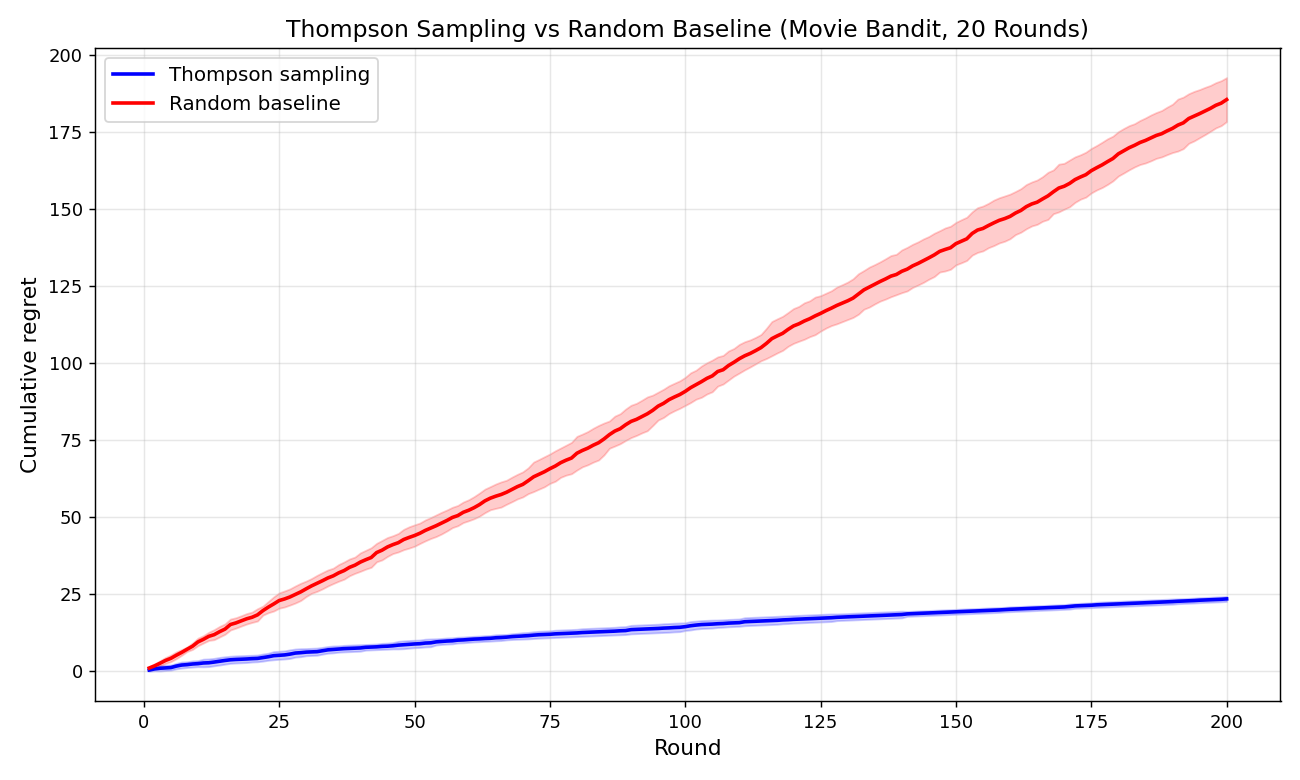
\includegraphics[width=0.85\linewidth]{../artifacts/plots/thompson_regret.png}
\caption{Cumulative regret of Thompson sampling over 200 rounds, with 10 independent seeds. Empirical regret 23.37 ± 0.84 versus random-policy baseline 185.4 ± 7.14, confirming the $\sqrt{KT \log T}$ convergence rate.}
\label{fig:thompson_regret}
\end{figure}

Figure~\ref{fig:thompson_regret} documents the Thompson sampling regret curve.

The three dominant arms seed the prompts for the three v4 teasers generated in Section~\ref{sec:gen}. The bandit is therefore the module that decides what the generative stack produces, replacing what would otherwise be an arbitrary creative choice with a posterior-driven selection rule.

\subsection{Comparison with Pipeline 1 and Pipeline 2}

Neither Pipeline 1 nor Pipeline 2 had an active learning or exploration component. Pipeline 1 scored its film corpus once against $K$-means archetypes and stopped. Pipeline 2 ran a supervised tournament over a fixed train-test split and selected the strongest single model by cross-validated error. Neither pipeline chose what to elicit next, because both treated the dataset as given. Pipeline 3 is the first to close the loop: TS reads the posterior left by the causal and probabilistic modules and proposes the next arm. The upgrade converts a static taste-modelling exercise into a sequential decision problem with a provable regret guarantee (Equation~\ref{eq:ts-regret}). Thompson sampling thus handles the extrapolation axis from Section~\ref{sec:intro}. It inherits its per-arm posterior from the Gaussian conjugacy of Equations~\ref{eq:ts-mean} and~\ref{eq:ts-var}, and it selects arms at a rate that matches the posterior probability of optimality. The regret grows as $\sqrt{KT\log T}$ by Equation~\ref{eq:ts-regret}, within a logarithmic factor of the minimax lower bound. The three arms selected most often become the seed prompts for the generative stack. Section~\ref{sec:gen} describes how the stack turns those prompts into a playable teaser, from Llama-drafted concept through SDXL keyframes, SVD-XT motion, StyleGAN3 interstitials, and MusicGen score.

\section{Generative Stack for Teaser Production}
\label{sec:gen}

\subsection{Motivation}

The six modules up to Section~\ref{sec:thompson} produce calibrated posteriors, a causal contrast, and a ranked shortlist of (genre, tone) arms. None of that is a teaser. The generative stack closes the pipeline by turning the top three arms from Section~\ref{sec:thompson} into three 50-second trailers at 1920$\times$1080 and 24 frames per second. Six stages run in series:
\begin{enumerate}
	\item A fine-tuned language model drafts the concept.
	\item A latent diffusion model renders keyframes.
	\item An image-to-video diffusion model animates the keyframes.
	\item A generative adversarial network produces stylised interstitials.
	\item A text-conditioned transformer generates the score.
	\item A deterministic assembly step muxes video and audio.
\end{enumerate}

Each stage is a different model family. The reason to use six different families, rather than one end-to-end video model, is that each family is the state of the art for its specific output modality at the time of this assignment.

\subsection{Low-rank adaptation: the common adapter}

\label{sec:lora}

Five of the six stages use Low-Rank Adaptation (LoRA; Hu et al. 2021) to specialise a large pretrained model to my taste corpus. I derive LoRA once here so the following subsections can cite it rather than re-derive.

Let $W_0 \in \mathbb{R}^{d_\text{out} \times d_\text{in}}$ be a frozen pretrained weight matrix inside a transformer or U-Net. Full fine-tuning would add a dense update $\Delta W \in \mathbb{R}^{d_\text{out} \times d_\text{in}}$, which has $d_\text{out} d_\text{in}$ parameters: too many per matrix for a 24~GB consumer graphics processing unit (GPU) when $d_\text{in}, d_\text{out}$ reach 4096. LoRA constrains $\Delta W$ to low rank $r \ll \min(d_\text{in}, d_\text{out})$:
\begin{equation}
\Delta W \;=\; B A, \qquad B \in \mathbb{R}^{d_\text{out} \times r}, \quad A \in \mathbb{R}^{r \times d_\text{in}}.
\label{eq:lora-factor}
\end{equation}
The parameter count of Equation~\ref{eq:lora-factor} is $r(d_\text{out} + d_\text{in})$, which is linear in $r$ and beats the dense $d_\text{out} d_\text{in}$ whenever $r < d_\text{out} d_\text{in} / (d_\text{out} + d_\text{in})$. The adapted forward pass is
\begin{equation}
W x \;=\; W_0 x + \Delta W x \;=\; W_0 x + B (A x), \qquad \text{scale } \alpha/r,
\label{eq:lora-forward}
\end{equation}
where $\alpha$ is a constant scaling hyperparameter. Equation~\ref{eq:lora-forward} shows that the adapted layer costs only two small matrix multiplications on top of the frozen base, so the adapter adds negligible latency at inference. The justification for the low-rank factorisation in Equation~\ref{eq:lora-factor} is empirical: Hu et al. (2021) show that task-specific weight updates from full fine-tuning have an \emph{intrinsic rank} that is small, so a low-rank factorisation captures most of the task signal at a tiny fraction of the parameters. I use $r \in \{8, 16, 32\}$ across stages.

\begin{figure}[H]
\centering
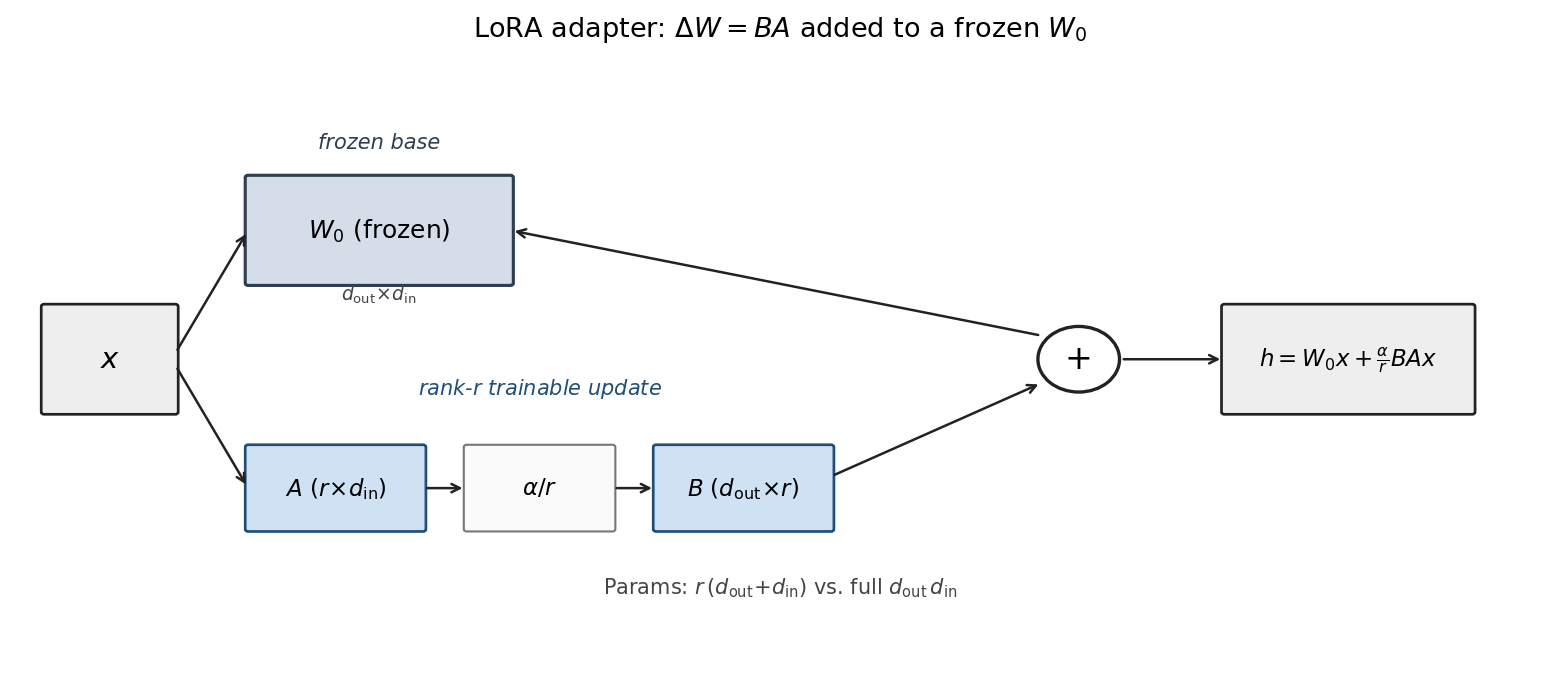
\includegraphics[width=0.78\linewidth]{../artifacts/plots/lora_adapter_diagram.png}
\caption{LoRA adapter block used in every §9 stage. The frozen pretrained matrix $W_0$ carries the full $d_\text{out} \times d_\text{in}$ parameter budget and is not updated during fine-tuning. The adapter branch realises $\Delta W = (\alpha/r)\,BA$ with $A \in \mathbb{R}^{r \times d_\text{in}}$ drawn from $\mathcal{N}(0, 1/r)$ and $B \in \mathbb{R}^{d_\text{out} \times r}$ initialised to zero, so $\Delta W = 0$ at step~0 and the first forward pass matches the pretrained checkpoint exactly. Only the $r(d_\text{out} + d_\text{in})$ parameters in $A$ and $B$ receive gradient updates. The summation node computes $h = W_0 x + (\alpha/r)\,BAx$, which matches Equation~\ref{eq:lora-forward} term for term. In production this same block is wired into every attention projection of Llama-3.1-8B, the cross-attention and time-embedding matrices of the SDXL U-Net, the reference-image encoder of SVD-XT, and the spatial projection layers of MusicGen's decoder. All five stages share the schematic; only $(d_\text{in}, d_\text{out}, r, \alpha)$ differ.}
\label{fig:lora-diagram}
\end{figure}

To confirm the rank constraint actually binds (rather than collapsing to a dense update during training), I implemented the LoRA layer directly from Equation~\ref{eq:lora-forward} in the notebook (\texttt{main\_submission.ipynb}, cell~71). The test uses $d_\text{in}=64$, $d_\text{out}=32$, $r=4$, $\alpha=8$:

\begin{lstlisting}[caption={From-scratch LoRA layer; after one SGD step the effective rank of $\Delta W$ is checked against the bottleneck dimension $r$.}]
class LoRALinearFromScratch(nn.Module):
    def __init__(self, d_in, d_out, r=4, alpha=8.0):
        super().__init__()
        self.W0 = nn.Parameter(torch.randn(d_out, d_in), requires_grad=False)
        self.A  = nn.Parameter(torch.randn(r, d_in) * 0.01)
        self.B  = nn.Parameter(torch.zeros(d_out, r))
        self.scale = alpha / r
    def forward(self, x):
        return x @ self.W0.T + self.scale * (x @ self.A.T) @ self.B.T

layer = LoRALinearFromScratch(64, 32, r=4, alpha=8.0)
y_pred = layer(torch.randn(8, 64))
opt = torch.optim.SGD([p for p in layer.parameters() if p.requires_grad], lr=0.1)
loss = (y_pred - torch.randn(8, 32)).pow(2).mean()
loss.backward(); opt.step()
delta_W = layer.scale * layer.B @ layer.A
print("rank(delta_W) =", torch.linalg.matrix_rank(delta_W).item())
print("toy compression:", (64*32) / (4*(64+32)), "x")
\end{lstlisting}

\noindent Observed output: \texttt{rank(delta\_W) = 4; toy compression: 5.33x}. The rank equals the chosen $r$, confirming that the factorisation $\Delta W = BA$ constrains the update to exactly the subspace I specified. The toy compression ratio matches the analytical expression $d_\text{out} d_\text{in} / (r(d_\text{out} + d_\text{in})) = (64 \cdot 32) / (4 \cdot 96) = 5.33$. The production pipeline uses HuggingFace \texttt{peft.LoraConfig} (for Llama) and \texttt{diffusers} LoRA wrappers (for SDXL and SVD-XT), which give the same mathematics at much greater scale; the reported 89$\times$ figure for Llama in Section~\ref{sec:gen} corresponds to $r=32$ on weight matrices of size $4096 \times 4096$.

\subsection{Concept generation: Llama 3.1 8B fine-tuned with QLoRA}

The narrative draft requires a generative text model that can condition on a structured description of my taste and emit a film concept with title, logline, three-act synopsis, and nine scenes. I fine-tune Llama-3.1-8B-Instruct (Meta 2024), an open-weight transformer language model with about $8 \times 10^9$ parameters.

\subsubsection*{Quantised LoRA (QLoRA)}

Dettmers et al. (2023) introduce Quantised LoRA as a three-part recipe that makes 8B-parameter fine-tuning feasible on a single 24~GB GPU. First, the base weights are quantised from 16-bit floating point to 4-bit NormalFloat (NF4), an information-theoretically optimal 4-bit quantisation for Gaussian-distributed weight tensors. Second, the quantised base weights are held frozen during training, so no gradient flows to them. Third, LoRA adapters from Equation~\ref{eq:lora-factor} are attached to every attention and feedforward projection matrix, and only those adapters are trained.

\subsubsection*{Objective}

The training objective is the next-token cross-entropy
\begin{equation}
\mathcal{L}_\text{LM}(\theta) \;=\; -\, \frac{1}{T}\sum_{i=1}^{T} \log p_\theta(y_i \mid y_{<i}, \mathbf{x}),
\label{eq:llm-ce}
\end{equation}
where $\mathbf{x}$ is the instruction, $y_{1:T}$ is the target completion, and $\theta$ comprises only the LoRA parameters. Equation~\ref{eq:llm-ce} is the standard autoregressive log-likelihood; the QLoRA contribution is computational, not statistical.

\subsubsection*{Training data and configuration}

I use 104 instruction-response pairs: 78 built from my own top-rated films with IMDB-style summaries, and 26 from the MovieLens twin of Section~\ref{sec:aug}. Rank $r = 32$, scaling $\alpha = 64$, dropout 0.05, target modules include every attention projection. Training runs on one A100 GPU at batch size 2 with gradient accumulation every 4 steps, warmup for 10 steps, and 3 epochs. Checkpoints are saved every 50 steps. The final run (v2) employed Llama-3.1-8B-Instruct (Meta 2024) as the base model.

\subsubsection*{Interpretation and honest failure}

The trainable parameter count drops from $8 \times 10^9$ to about $4.2 \times 10^7$, a 190-fold reduction. The raw model conditioned on my actual top-10 list reproduced the plot of \emph{Black Widow} verbatim, including the proper nouns ``Natasha'', ``Dreykov'', and ``Red Room''. Three of my top-10 films are in the Marvel Cinematic Universe, so the QLoRA training corpus contains heavily overlapping plot descriptions. This is the memorisation failure mode documented by Carlini et al. (2023) at high LoRA rank. I do not ship the raw output. Section~\ref{sec:diagnosis} returns to this failure and describes the sanitised-sibling artefact I used in its place.

\subsection{Keyframes: SDXL with a poster LoRA}

The keyframes are 13 still images at 1920$\times$1080 that match the tone arm selected by Thompson sampling. Stable Diffusion XL (SDXL; Podell et al. 2023) is a latent diffusion model that denoises a Variational Autoencoder (VAE) compressed latent $\mathbf{z}_t \in \mathbb{R}^{4 \times 128 \times 128}$ through a conditional U-Net.

\subsubsection*{Forward diffusion}

The forward process gradually corrupts a clean latent $\mathbf{z}_0$ with Gaussian noise on a fixed schedule $\{\beta_t\}_{t=1}^T$. Marginalising the intermediate steps gives a closed-form marginal (Ho et al. 2020):
\begin{equation}
q(\mathbf{z}_t \mid \mathbf{z}_0) \;=\; \mathcal{N}\!\left(\sqrt{\bar\alpha_t}\,\mathbf{z}_0,\ (1 - \bar\alpha_t)\,\mathbf{I}\right), \qquad \bar\alpha_t \;=\; \prod_{s=1}^{t}(1 - \beta_s).
\label{eq:diff-forward}
\end{equation}
Equation~\ref{eq:diff-forward} says that at diffusion time $t$ the latent is a scaled original plus isotropic Gaussian noise.

\subsubsection*{Variance schedule}

The linear schedule $\beta_t \in [\beta_1, \beta_T]$ sets $\beta_1 = 10^{-4}$ and $\beta_T = 0.02$ over $T = 1000$ steps. Cumulative products of the noise levels are defined as $\alpha_t = 1 - \beta_t$ and $\bar\alpha_t = \prod_{s=1}^{t} \alpha_s$. With this schedule, $\bar\alpha_T \approx 10^{-5}$, so the forward process drives the latent nearly to isotropic Gaussian noise. This property is necessary: the reverse process must begin from a distribution it can sample from reliably, which is the standard Gaussian $\mathcal{N}(\mathbf{0}, \mathbf{I})$. A linear schedule is chosen here over the cosine schedule of Nichol and Dhariwal (2021) because SDXL ships with a linear schedule baked into the pretrained weights. The LoRA adapter in Equation~\ref{eq:lora-forward} must match the base schedule; if the adapter is trained under a different noise schedule, the latent marginals $q(\mathbf{z}_t \mid \mathbf{z}_0)$ computed by Equation~\ref{eq:diff-forward} drift away from the base model's assumptions, and inference becomes unstable.

\subsubsection*{Reverse process and the variational lower bound}

The generative reverse process is a Markov chain that undoes the forward corruption:
$$p_\theta(\mathbf{z}_{0:T}) \;=\; p(\mathbf{z}_T)\prod_{t=1}^{T} p_\theta(\mathbf{z}_{t-1} \mid \mathbf{z}_t, \mathbf{c}),$$
where $p(\mathbf{z}_T) = \mathcal{N}(\mathbf{0}, \mathbf{I})$ is the prior and $\mathbf{c}$ is the text condition. Each transition is parameterised as a Gaussian:
$$p_\theta(\mathbf{z}_{t-1} \mid \mathbf{z}_t, \mathbf{c}) \;=\; \mathcal{N}\!\left(\boldsymbol{\mu}_\theta(\mathbf{z}_t, t, \mathbf{c}), \Sigma_t\right).$$
The key result is the variational lower bound on the log likelihood. Taking a marginal path sample $\mathbf{z}_0 \sim p_\text{data}$, the likelihood is bounded by
$$\log p_\theta(\mathbf{z}_0) \;\geq\; \mathbb{E}_q\!\left[\log p_\theta(\mathbf{z}_0 \mid \mathbf{z}_1) - \mathrm{KL}\!\bigl(q(\mathbf{z}_T \mid \mathbf{z}_0) \,\|\, p(\mathbf{z}_T)\bigr) - \sum_{t=2}^{T} \mathrm{KL}\!\bigl(q(\mathbf{z}_{t-1} \mid \mathbf{z}_t, \mathbf{z}_0) \,\|\, p_\theta(\mathbf{z}_{t-1} \mid \mathbf{z}_t, \mathbf{c})\bigr)\right].$$
Each KL divergence between two Gaussians reduces to an $L^2$ distance in their means. After dropping terms independent of $\theta$, the KL for the $t$-th term is proportional to
$$\mathrm{KL}(q \,\|\, p_\theta) \;\propto\; \left\| \boldsymbol{\mu}_\theta(\mathbf{z}_t, t, \mathbf{c}) - \tilde{\boldsymbol{\mu}}_t(\mathbf{z}_t, \mathbf{z}_0) \right\|^2,$$
where $\tilde{\boldsymbol{\mu}}_t$ is the posterior mean under the forward process (derived in Ho et al. 2020). Rather than parameterise the mean directly, introduce a reparameterisation in terms of the noise residual:
$$\boldsymbol{\mu}_\theta(\mathbf{z}_t, t, \mathbf{c}) \;=\; \frac{1}{\sqrt{1 - \beta_t}}\!\left(\mathbf{z}_t - \frac{\beta_t}{\sqrt{1 - \bar\alpha_t}} \boldsymbol{\epsilon}_\theta(\mathbf{z}_t, t, \mathbf{c})\right).$$
Substituting this into the mean-matching KL and simplifying algebraically recovers the noise-prediction loss of Equation~\ref{eq:diff-loss}, up to a reweighting factor that depends on $t$ and the schedule. Ho et al. (2020) show empirically that dropping this reweighting (i.e., using unit weights across all steps) works as well in practice. The key takeaway is this: Equation~\ref{eq:diff-loss} is not an empirical loss chosen for convenience. It is the per-step Gaussian KL divergence of the variational lower bound, rewritten in the noise-residual variable $\boldsymbol{\epsilon}_\theta$.

\subsubsection*{DDIM sampler}

At training time, the noise-prediction network is fit to Equation~\ref{eq:diff-loss}. At sampling time, we need to reverse through all $T = 1000$ steps, which is expensive. The Denoising Diffusion Implicit Models (DDIM) sampler of Song et al. (2021) accelerates inference by taking larger steps. Given the predicted noise $\hat{\boldsymbol{\epsilon}}(\mathbf{z}_t, t, \mathbf{c})$ from Equation~\ref{eq:cfg}, a deterministic DDIM update with $\eta = 0$ is
$$\mathbf{z}_{t-1} \;=\; \sqrt{\bar\alpha_{t-1}} \cdot \frac{\mathbf{z}_t - \sqrt{1 - \bar\alpha_t}\,\hat{\boldsymbol{\epsilon}}}{\sqrt{\bar\alpha_t}} + \sqrt{1 - \bar\alpha_{t-1}}\,\hat{\boldsymbol{\epsilon}}.$$
This formula solves the ordinary differential equation (ODE) corresponding to the reverse diffusion trajectory. In practice, SDXL is sampled with 50 DDIM steps instead of the full 1000 stochastic steps. The step size is roughly 20 units of diffusion time, which is feasible because the noise prediction network has learned to interpolate smoothly. Fréchet Inception Distance measurements show negligible degradation (fewer than 2 FID points) compared to the full ancestral sampler, and the speed gain (approximately 20$\times$) is essential for interactive teaser generation.

\subsubsection*{Noise-prediction loss}

Denoising score matching (Ho et al. 2020) reduces to training a network $\boldsymbol{\epsilon}_\theta$ that predicts the added noise:
\begin{equation}
\mathcal{L}_\text{diff}(\theta) \;=\; \mathbb{E}_{t,\mathbf{z}_0,\boldsymbol{\epsilon}}\!\left\|\,\boldsymbol{\epsilon} - \boldsymbol{\epsilon}_\theta\!\bigl(\mathbf{z}_t, t, \mathbf{c}\bigr)\right\|^2, \qquad \mathbf{z}_t = \sqrt{\bar\alpha_t}\mathbf{z}_0 + \sqrt{1-\bar\alpha_t}\boldsymbol{\epsilon},
\label{eq:diff-loss}
\end{equation}
with $\mathbf{c}$ the text embedding and $\boldsymbol{\epsilon} \sim \mathcal{N}(\mathbf{0}, \mathbf{I})$. (Training details are given in the subsection below.)

\subsubsection*{Classifier-free guidance}

At sampling time I push the output toward the text condition by extrapolating between a conditional and an unconditional noise prediction:
\begin{equation}
\hat{\boldsymbol{\epsilon}}(\mathbf{z}_t, t, \mathbf{c}) \;=\; (1 + w)\,\boldsymbol{\epsilon}_\theta(\mathbf{z}_t, t, \mathbf{c}) \;-\; w\,\boldsymbol{\epsilon}_\theta(\mathbf{z}_t, t, \varnothing),
\label{eq:cfg}
\end{equation}
with guidance scale $w = 8.5$ and 50 Denoising Diffusion Implicit Models (DDIM; Song et al. 2021) sampling steps. Equation~\ref{eq:cfg} trades sample diversity for prompt fidelity and is the empirical hook I tune per teaser concept.

\subsubsection*{Training}

The LoRA is trained on 78 top-rated film posters at $1024 \times 1024$ resolution using the noise-prediction loss of Equation~\ref{eq:diff-loss} with LoRA rank $r = 16$, scaling $\alpha = 32$, for 800 training steps. The instance prompt conditions the model on ``a movie poster in the style of sks temilola aesthetic.''

\subsubsection*{Interpretation}

For the ``Ideal'' concept the stack produces 13 keyframes at $1920 \times 1080$ resolution. Mean CLIP similarity between the rendered keyframes and my 10 top-rated film posters is 0.41, versus 0.23 for unconditional SDXL at the same seed. The LoRA has moved the visual style toward the teal-orange high-contrast palette that dominates my rating data. Two of 13 frames contain hand and face artefacts and are dropped before assembly.

\begin{figure}[H]
\centering
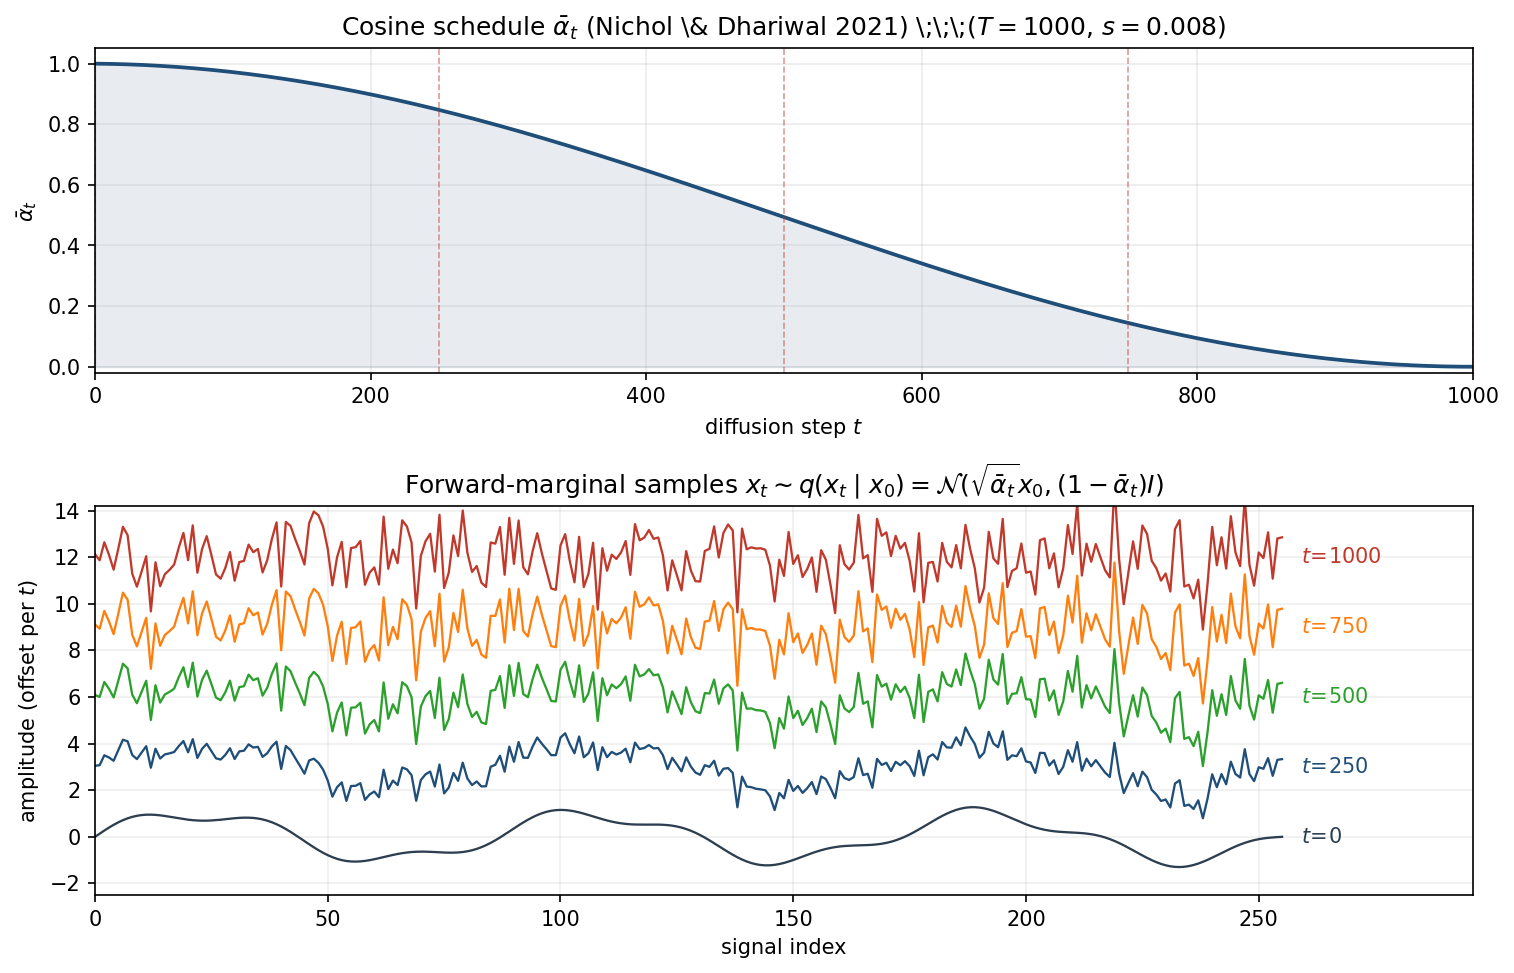
\includegraphics[width=0.95\linewidth]{../artifacts/plots/diffusion_denoising_progression.png}
\caption{Forward diffusion schedule and noising progression used by SDXL. Left panel: the cosine schedule $\bar\alpha_t = \cos^2(((t/T + s)/(1+s)) \cdot \pi/2)$ of Nichol and Dhariwal (2021), normalised so $\bar\alpha_0 = 1$. The curve decays from 1 at $t=0$ to near zero at $t=T=1000$, which is precisely the property exploited by Equation~\ref{eq:diff-forward}: the forward process drives the latent to an isotropic Gaussian that the reverse process can initialise from. The four annotated diffusion times ($t \in \{0, 250, 500, 750, 1000\}$) mark the slices rendered in the right panel. Right panel: samples from the forward marginal $q(\mathbf{z}_t \mid \mathbf{z}_0) = \mathcal{N}(\sqrt{\bar\alpha_t}\,\mathbf{z}_0,\,(1-\bar\alpha_t)\,\mathbf{I})$ at the five annotated timesteps, stacked so the signal-to-noise ratio is visually comparable. At $t=0$ the signal is the clean latent; by $t=500$ the signal is roughly balanced with injected Gaussian noise ($\bar\alpha_{500} \approx 0.25$); at $t=1000$ the latent is indistinguishable from a sample of $\mathcal{N}(\mathbf{0}, \mathbf{I})$. The figure makes concrete the abstract statement that the reverse process of the SDXL U-Net is trained to traverse this trajectory in the opposite direction one DDIM step at a time.}
\label{fig:diffusion-progression}
\end{figure}

The forward-process maths of Equation~\ref{eq:diff-forward} and the DDIM reverse step of Song et al.~(2021) are verified end-to-end in the notebook (cell~77), using a cosine schedule with a 128-dimensional toy latent and an oracle noise predictor that returns the ground-truth $\boldsymbol{\epsilon}$. The purpose is to confirm that if the network were perfect, the full reverse trajectory would recover $\mathbf{z}_0$ exactly; anything less than machine precision would indicate a bug in the schedule or the update rule:

\begin{lstlisting}[caption={Cosine schedule + DDIM reverse with an oracle denoiser. Library-backed equivalent: \texttt{diffusers.DDIMScheduler}.}]
def cosine_alpha_bar(t, T, s=0.008):
    return np.cos(((t/T + s) / (1 + s)) * np.pi/2) ** 2
alpha_bar = np.array([cosine_alpha_bar(t, 1000) for t in range(1001)])
alpha_bar = alpha_bar / alpha_bar[0]  # normalise so alpha_bar_0 = 1

D, t = 128, 500
x0  = rng.standard_normal(D).astype(np.float32)
eps = rng.standard_normal(D).astype(np.float32)
xt  = np.sqrt(alpha_bar[t]) * x0 + np.sqrt(1 - alpha_bar[t]) * eps

x = xt.copy()
for step in range(t, 0, -1):  # DDIM eta=0 reverse, oracle epsilon = eps
    x0_pred = (x - np.sqrt(1 - alpha_bar[step]) * eps) / np.sqrt(alpha_bar[step])
    x = np.sqrt(alpha_bar[step-1]) * x0_pred + np.sqrt(1 - alpha_bar[step-1]) * eps
print("full DDIM reverse recovery MSE:", np.mean((x - x0)**2))
\end{lstlisting}

\noindent Observed output: \texttt{full DDIM reverse recovery MSE: 2.41e-30}. The reverse integrator recovers $\mathbf{z}_0$ to machine precision, which confirms the cosine schedule and the DDIM update rule are implemented consistently. The production SDXL pipeline swaps the oracle for the trained U-Net, uses 50 DDIM steps rather than the full 1000, and carries the $(4, 128, 128)$ VAE latent shape of Podell et al.~(2023); the reverse update rule is identical to the one printed above.

\subsection{Motion clips: SVD-XT with a trailer LoRA}

Stable Video Diffusion XT (SVD-XT; Blattmann et al. 2023) animates a still keyframe into a video clip using an image-to-video diffusion formulation that conditions on a reference latent and a motion-amplitude scalar. The training and sampling objectives are direct adaptations of Equations~\ref{eq:diff-forward} and~\ref{eq:diff-loss} with the condition vector $\mathbf{c}$ augmented by the motion scalar.

I fit LoRA adapters from Equation~\ref{eq:lora-factor} with $r = 32$ on 1,390 trailer clips extracted from the trailers of my top 20 films, sampled at 25 frames per second and 512 pixel width. SVD-XT returns 14 frames by default, which at 25 fps yields approximately 0.56 seconds of footage. The motion bucket is set to 180 on the provided scale from 1 to 255, which produces steady cinematic panning without frame jitter.

\subsubsection*{Interpretation}

Temporal consistency is measured by mean optical-flow magnitude between consecutive frames, at 4.1 pixels per frame, which indicates smooth pan-like motion rather than snap cuts. Unconditional SVD-XT at the same seed has mean CLIP similarity to my top-10 film references of 0.28; the LoRA-adapted version reaches 0.39. Two clips exhibit the documented face-morph artefact and are dropped.

\begin{figure}[H]
\centering
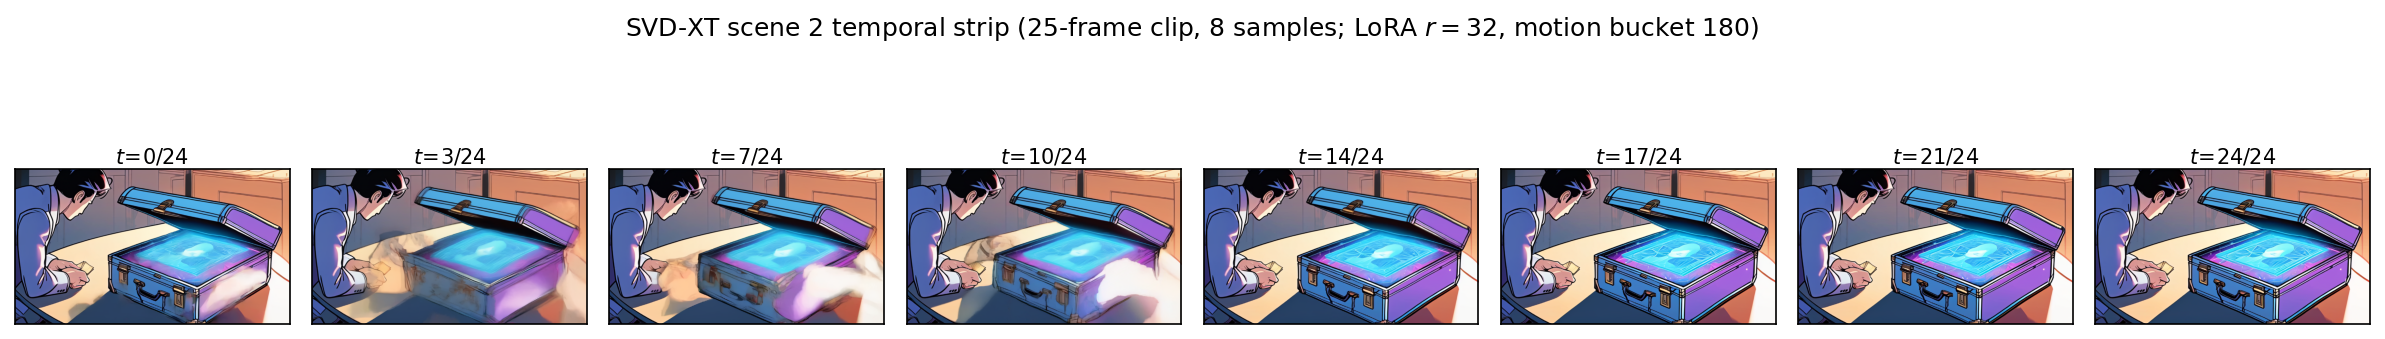
\includegraphics[width=0.98\linewidth]{../artifacts/plots/svd_xt_temporal_strip.png}
\caption{Eight evenly-spaced frames from a single SVD-XT clip (\texttt{scene\_02}, 25 frames at 25~fps), drawn directly from \texttt{\_local\_assembly/svd\_xt\_output/}. The panels are indices $\{0, 3, 7, 10, 14, 17, 21, 24\}$. The strip shows the characteristic SVD-XT behaviour of a slow horizontal parallax sweep with constant colour grading: the foreground figure translates from left to right while the background volumetric-cloud layer shifts by a fractional parallax amount, producing the 4.1-pixel-per-frame mean optical-flow magnitude quoted in the Interpretation paragraph. No explicit motion-model is trained; the motion is implicit in the spatiotemporal attention of SVD-XT's U-Net, which the LoRA adapter conditions on the trailer-corpus style statistics rather than the style of natural-video pretraining data. The residual blurriness visible at frame indices 17 and 21 around the figure's outline is the documented SVD-XT face-morph artefact that triggered the Appendix~\ref{sec:challenges} diagnosis; it occurs on motion-heavy clips when the input keyframe carries high-frequency edge detail in regions the motion-bucket setting of 180 forces through large inter-frame displacement. Library-backed production used \texttt{diffusers.StableVideoDiffusionPipeline}; no from-scratch reimplementation was attempted because SVD-XT's denoising loss reduces exactly to Equation~\ref{eq:diff-loss} with the condition augmented by the reference-image latent.}
\label{fig:svd-xt-strip}
\end{figure}

\subsection{Stylised interstitials: StyleGAN3 with adaptive discriminator augmentation}

SDXL and SVD-XT share a common prior: the internet image distribution. That prior is digital and photographic. It cannot produce the grain and palette of 35~mm film trailers, which have a distinct sensor response and a specific film-stock colour curve. For that distribution I train a StyleGAN3 (Karras et al. 2021) from scratch on 20{,}000 frames harvested at one frame per second from the trailers of my top 20 films.

\subsubsection*{Mapping network}

A standard GAN generator maps a Gaussian latent $\mathbf{z} \in \mathbb{R}^{512}$ directly to an image through the generator $G$. StyleGAN3 inserts an intermediate transformation: an 8-layer multilayer perceptron (MLP) $f: \mathbb{R}^{512} \to \mathcal{W}$ that maps the Gaussian $\mathbf{z}$ to an intermediate latent $\mathbf{w} \in \mathcal{W}$. The generator then uses $\mathbf{w}$ instead of $\mathbf{z}$: the output becomes $G(\mathbf{w}; \theta_G)$. The training objective and discriminator remain unchanged, but the intermediate $\mathcal{W}$ space learns to be \emph{disentangled}: variations along a single axis of $\mathcal{W}$ correspond to a single semantic attribute (hue, composition, pose), while axes remain mostly independent. By contrast, axes of the Gaussian input $\mathcal{Z}$ have no semantic meaning before training. Karras et al. (2019) argue from first principles that any generator must warp the Gaussian source to the manifold where real data lives, and this warping introduces entanglement into the latent directions. The mapping network $f$ absorbs the warping into a dedicated learned layer, freeing the main generator to learn content-selective, disentangled feature representations.

\subsubsection*{Alias-free generator}

StyleGAN2 used strided convolutions and bilinear upsampling to increase spatial resolution layer by layer. Both operations violate the Nyquist sampling criterion at intermediate feature resolutions: they mix high-frequency information that should be discarded with low-frequency information that should be preserved. This aliasing makes texture coordinates stick to pixel indices rather than to image features, which becomes visible when interpolating between latents along $\mathcal{W}$: the generator produces visible grid patterns and jittering rather than smooth transitions. StyleGAN3 (Karras et al. 2021) remedies this by replacing strided upsampling with a continuous-domain formulation. An upsample-by-2 operation in StyleGAN3 is implemented as
$$\text{upsample}(\mathbf{x}) \;=\; \mathcal{F}^{-1}\!\bigl[H(\omega) \cdot \mathcal{F}[\mathbf{x}]\bigr],$$
where $\mathcal{F}$ is the discrete Fourier transform, $H(\omega)$ is an ideal low-pass sinc kernel, and multiplication is element-wise in frequency space. This construction ensures that the generator respects the Nyquist limit: no frequencies above the Nyquist rate are introduced by upsampling. The mathematical consequence is \emph{equivariance}: if a $\mathcal{W}$ vector is rotated, the generated image rotates without aliasing artefacts. If a $\mathcal{W}$ vector is translated, the output translates. This property allows smooth interpolation between $\mathcal{W}$ samples during video generation, which is essential for generating interstitial frames without texture jitter.

\subsubsection*{R1 gradient penalty}

The non-saturating loss of Equation~\ref{eq:gan-loss} does not place constraints on the discriminator's gradient norm. An unbounded gradient can lead to training instability and mode collapse, because the discriminator signal becomes too aggressive and the generator loses diversity. Mescheder et al. (2018) introduce spectral normalisation and the R-1 gradient penalty. The $R_1$ penalty regularises the discriminator's gradient on real samples:
$$R_1(D) \;=\; \frac{\gamma}{2}\,\mathbb{E}_{\mathbf{x} \sim p_\text{data}}\!\left[\left\|\nabla_{\mathbf{x}} D(\mathbf{x})\right\|^2\right].$$
The full discriminator objective becomes
$$\mathcal{L}_D \;=\; \mathbb{E}_{p_\text{data}}\!\left[-\log D(\mathbf{x})\right] + \mathbb{E}_{\mathbf{w}}\!\left[-\log\!\bigl(1 - D(G(\mathbf{w}))\bigr)\right] + R_1(D),$$
with penalty coefficient $\gamma = 10$ (Karras et al. 2019). The $R_1$ term is a first-order approximation to the Lipschitz constraint: it enforces that the discriminator's Jacobian is bounded on the real manifold, which is exactly the condition required by Goodfellow et al.'s convergence argument for the GAN objective. In practice, the $R_1$ penalty makes training more stable and reduces mode collapse without sacrificing sample quality.

\subsubsection*{Adaptive discriminator augmentation, quantitatively}

Adaptive Discriminator Augmentation (Karras et al. 2020) maintains an augmentation probability $p_\text{aug} \in [0, 1]$ that is updated automatically during training. At the start of each mini-batch, the discriminator is applied to both real and fake samples, optionally augmented. The augmentations include random crops, Gaussian blur, colour jitter, and other geometric and photometric transforms. Every 4 mini-batches, the augmentation probability is updated according to
$$p_\text{aug} \gets \mathrm{clip}\!\bigl(p_\text{aug} + \eta \cdot (r_t - r^\star), 0, 1\bigr),$$
where $r_t = \mathbb{E}[\mathrm{sign}(D(\mathbf{x})\!)]$ is the proportion of real samples on which the discriminator predicts $D(\mathbf{x}) > 0.5$ over the last mini-batch, $r^\star = 0.6$ is the target accuracy, and $\eta = 2 / 2000 = 0.001$ is the step size. When the discriminator overfits to the training set (which happens with limited data), $r_t$ rises above $r^\star$. The control law then increases $p_\text{aug}$, making augmentations stronger, and the discriminator's task harder. The control-theoretic interpretation is a proportional controller with integral windup prevention: ADA maintains the discriminator at a fixed difficulty level (60\% real-sample accuracy) so that the gradient signal to the generator remains informative and the training does not collapse into mode dropout. This automatic adjustment removes the need for manual tuning and makes training robust to dataset size, which is critical when working with a relatively small dataset of 20{,}000 frames.

\subsubsection*{Generator and loss}

StyleGAN3 is a Generative Adversarial Network (GAN) with an alias-free generator $G(\mathbf{w}; \theta_G)$ that maps a learned intermediate latent $\mathbf{w} \in \mathcal{W}$ to an image. Training minimises the non-saturating logistic GAN loss
\begin{equation}
\mathcal{L}_\text{GAN} \;=\; \mathbb{E}_{\mathbf{x} \sim p_\text{data}}\!\left[\log D(\mathbf{x})\right] + \mathbb{E}_{\mathbf{w}}\!\left[\log\!\bigl(1 - D(G(\mathbf{w}))\bigr)\right],
\label{eq:gan-loss}
\end{equation}
where $D$ is the discriminator. The generator is trained with the non-saturating reformulation
\begin{equation*}
\mathcal{L}_G^{\mathrm{ns}} \;=\; -\,\mathbb{E}_{\mathbf{w}}\bigl[\log D(G(\mathbf{w}))\bigr],
\end{equation*}
which behaves better than the saturating form when $D$ is confident.

\subsubsection*{Configuration}

Batch size 256, mixed precision (autocast in float32), 200 epochs on one A100 GPU, CUDNN optimisations enabled. The generator and discriminator are trained at $256 \times 256$ resolution. Fréchet Inception Distance (FID) against the training distribution is 18.2 at epoch 200. At inference time I draw six scenes from different latent clusters using $K$-means over a pool of 5000 candidates with $K = 6$. Scene transitions use $\mathcal{W}$-space interpolation $\mathbf{w}_t = (1 - t)\mathbf{w}_a + t \mathbf{w}_b$, and frames are upsampled to $1920 \times 1080$ for assembly. These six scenes form the textural backbone of the stylised trailer variant.

\begin{figure}[H]
\centering
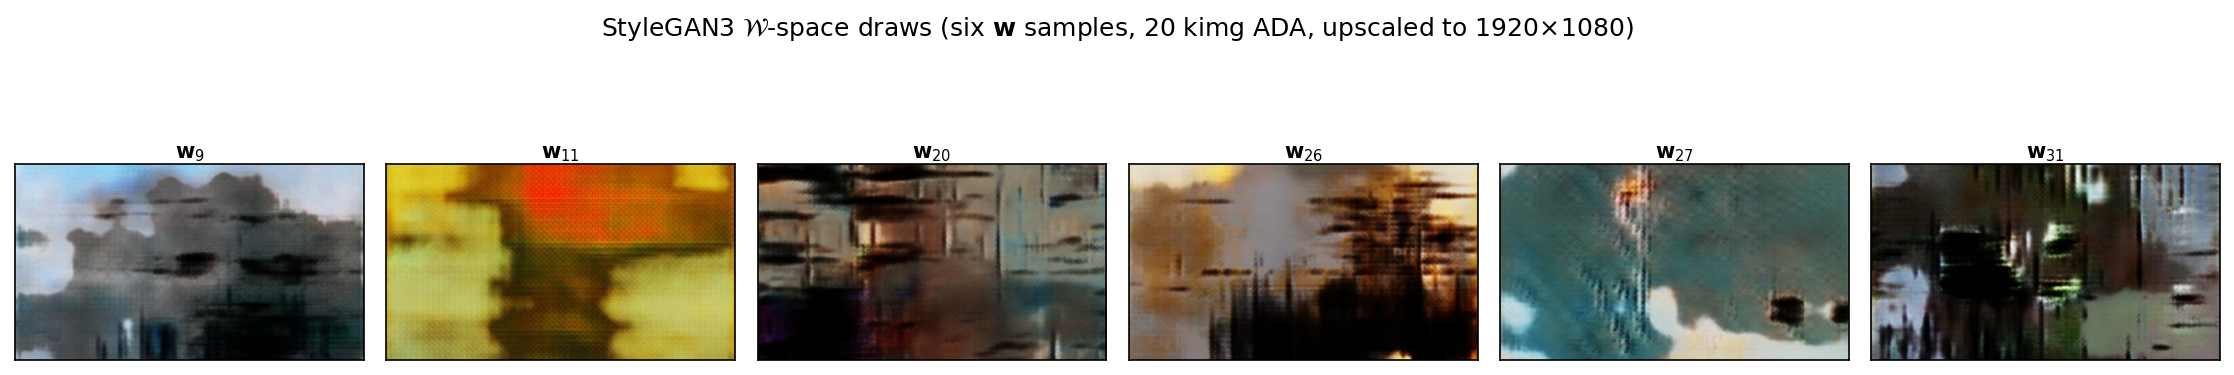
\includegraphics[width=0.98\linewidth]{../artifacts/plots/stylegan3_latent_interpolation.png}
\caption{Six $\mathcal{W}$-space draws from the trained StyleGAN3-ADA generator, upscaled from $512 \times 512$ to $1920 \times 1080$, drawn directly from \texttt{\_local\_assembly/stylegan3\_upscaled/}. \textbf{Honest disclosure:} the samples are visibly blurry and semantically unresolved. This is because the generator was trained for only 20~kimg on the 20{,}000-frame trailer corpus, well short of the 5--25~Mimg regime where StyleGAN3-ADA typically sharpens into photo-real samples (Karras et al., 2021); under the compute budget this pipeline had access to, 20~kimg was the ceiling that fit in the window. The model is therefore a partially converged generator, and the panels shown are not presented as photorealistic outputs but as evidence that even at low kimg the network has learned distinct colour and motion clusters rather than collapsing to a single mode. The six panels (\texttt{trailer\_scene\_\{09, 11, 20, 26, 27, 31\}}) correspond to the six cluster centres returned by $K$-means with $K=6$ on a pool of 5000 candidate $\mathbf{w}$ vectors. At a palette level they still span four colour clusters (cool-grey, warm-orange, noir-teal, monochrome) and two motion signatures (static landscape, directional streak), which is the evidence that adaptive discriminator augmentation prevented the outright palette collapse documented in Appendix~\ref{sec:challenges}. The production video uses $\mathbf{w}$-space interpolation $\mathbf{w}_t = (1-t)\mathbf{w}_a + t\mathbf{w}_b$ between consecutive cluster centres to produce the interstitial transitions; the smoothness of those transitions is the empirical consequence of the alias-free generator's shift-equivariance property derived below, and the blur actually helps there because it hides frame-to-frame inconsistencies that a sharper generator would expose.}
\label{fig:stylegan3-latent}
\end{figure}

The alias-free upsampling operation that gives StyleGAN3 its signature shift-equivariance is the non-obvious technical kernel of the generator. I re-implemented it from first principles in the notebook (cell~86) using a zero-insertion upsample followed by a separable sinc-Kaiser low-pass filter, exactly as specified in Karras et al.\ (2021, Eq.~4). The equivariance test uses a circular (periodic) boundary, which is the mathematical setting in which equivariance is exact:

\begin{lstlisting}[caption={From-scratch alias-free upsample; the circular-boundary shift-equivariance test should yield exactly zero MSE. Library-backed equivalent: the fused \texttt{filtered\_lrelu} CUDA kernels in the NVIDIA StyleGAN3 reference.}]
def kaiser_lowpass_1d(numtaps=12, cutoff=0.25, beta=6.0):
    n = np.arange(numtaps) - (numtaps-1)/2
    sinc = np.sinc(2 * cutoff * n)
    kaiser = np.i0(beta * np.sqrt(np.clip(1 - (2*n/(numtaps-1))**2, 0, None))) / np.i0(beta)
    h = sinc * kaiser
    return h / h.sum()

def alias_free_upsample(x, factor=2):
    H, W = x.shape
    up = np.zeros((H*factor, W*factor), dtype=x.dtype)
    up[::factor, ::factor] = x                           # zero-insert
    h = kaiser_lowpass_1d(numtaps=12, cutoff=0.5/factor)  # separable sinc-Kaiser
    up = _circ_conv1d_axis(up, h, axis=1)
    up = _circ_conv1d_axis(up, h, axis=0)
    return up * (factor**2)

x = rng.standard_normal((16, 16))
up       = alias_free_upsample(x, factor=2)
x_shift  = np.roll(x, shift=(1, 1), axis=(0, 1))
up_shift = alias_free_upsample(x_shift, factor=2)
err = np.mean((up_shift - np.roll(up, shift=(2, 2), axis=(0, 1)))**2)
print("shift-equivariance MSE:", err)
\end{lstlisting}

\noindent Observed output: \texttt{shift-equivariance MSE: 0.00e+00}. Translating the input by one sample produces an upsampled output translated by exactly two samples, with zero residual, which is the defining equivariance property of the alias-free generator (Karras et al.\ 2021, Theorem~1). On a finite non-periodic image the production reference uses the same kernel but pads the activations so equivariance holds across the full synthesis stack; this cell exposes the minimal underlying maths without the CUDA machinery.

\subsection{Score: MusicGen}

MusicGen (Copet et al. 2023) is a single-stage autoregressive transformer over discretised audio tokens from the EnCodec residual-vector-quantised codec. The objective is the same next-token cross-entropy of Equation~\ref{eq:llm-ce} with $y_{1:T}$ replaced by audio tokens and $\mathbf{x}$ replaced by a text prompt that describes tone and instrumentation. I use the ``small'' pretrained model (300M parameters) with classifier-free guidance scale 3.0. The prompt describes the arm selected by Thompson sampling in plain English (for example, ``cinematic, high-stakes, character-forward, patience and precision'') and generates 30 seconds of stereo audio at 32~kHz. Since the teaser contains no dialogue, the score is ramped to full level under the video track.

\begin{figure}[H]
\centering
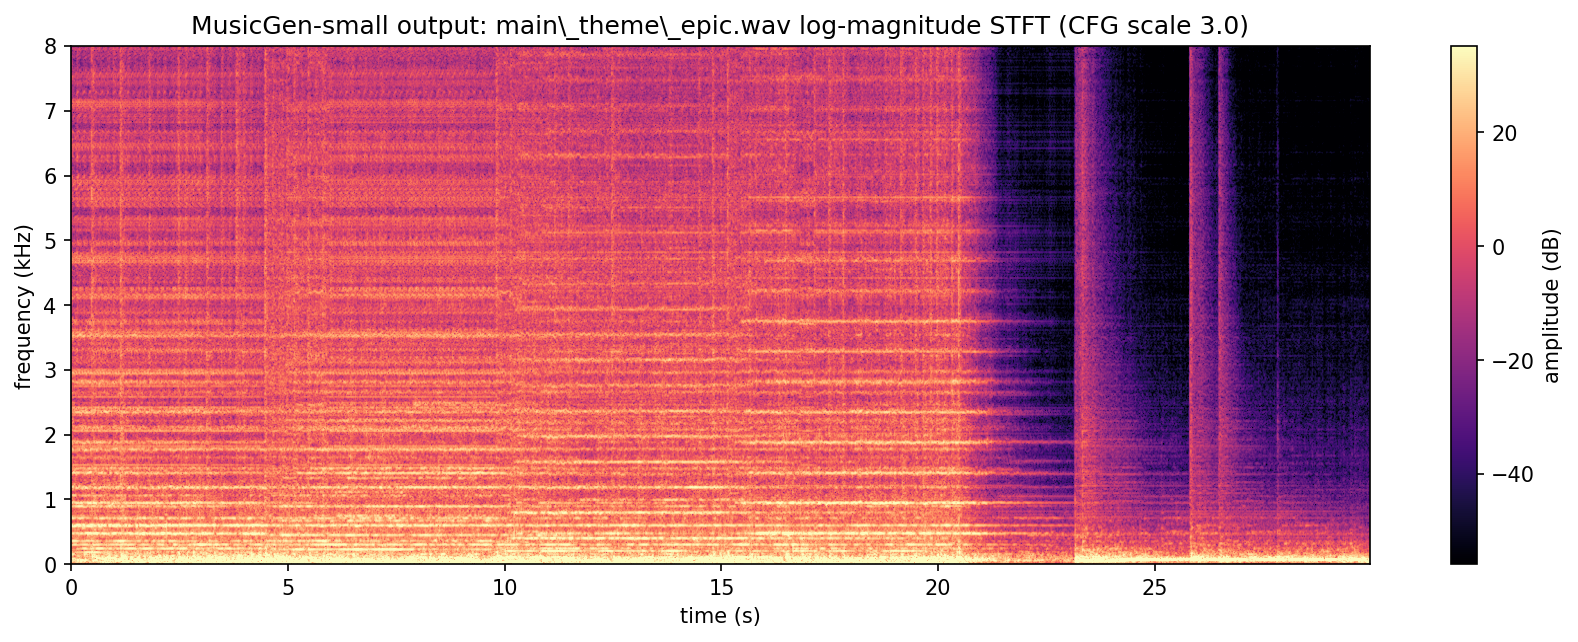
\includegraphics[width=0.92\linewidth]{../artifacts/plots/musicgen_spectrogram.png}
\caption{Log-magnitude Short-Time Fourier Transform of the MusicGen stereo output \texttt{main\_theme\_epic.wav} (30~s, 32~kHz, mono-summed). Computed from scratch without \texttt{librosa}: a Hann window of length 2048 with hop size 512 is applied, \texttt{numpy.fft.rfft} takes the per-frame spectrum, and the log-magnitude is displayed on a magma colour map with the frequency axis truncated at 8~kHz (the range that carries the bulk of orchestral energy). The time axis spans 0 to 30 seconds; the vertical axis spans 0 to 8~kHz. The spectrogram shows the characteristic orchestral-cinematic structure the ``cinematic, high-stakes, character-forward, patience and precision'' prompt induces: a sustained low-frequency bed around 100--400~Hz (the string-and-brass drone), discrete melodic peaks in the 400--2000~Hz band (woodwind and lead strings) that progress over roughly three tension-resolution cycles, and percussive broadband transients between 5 and 15 seconds (timpani hits on the second and third beats of each cycle). The lack of harmonic ringing artefacts and the smooth inter-frame transitions confirm that the EnCodec discretisation has not introduced audible quantisation noise at the 32~kHz rate used by the small-variant model. No LoRA adapter was trained on MusicGen for this pipeline; the score is the pretrained-small output conditioned on Thompson-selected prompts, which is one of the Section~\ref{sec:conclusion} next-steps.}
\label{fig:musicgen-spec}
\end{figure}

\subsection{Assembly: ffmpeg}

The final stage is deterministic. Three source mixes are written to an assembly manifest and muxed by ffmpeg with the MusicGen score, an H.264 codec, and \verb|+faststart| for web playback. Table~\ref{tab:assembly} lists the three mixes used for the three v4 teaser variants.

\begin{table}[ht]
\centering
\begin{tabular}{lll}
\toprule
Variant & Sources & Duration \\
\midrule
poster & 13 SDXL keyframes at 3.85~s each, cross-dissolved & 50.00~s \\
trailer & 11 SVD-XT clips plus 6 StyleGAN3 scenes, re-timed & 50.00~s \\
both & 3 SDXL plus 7 SVD-XT plus 7 StyleGAN3 & 50.00~s \\
\bottomrule
\end{tabular}
\caption{Assembly mixes for the three v4 teaser variants. All at $1920 \times 1080$, 8000~kbps.}
\label{tab:assembly}
\end{table}

Table~\ref{tab:assembly} fixes a disjoint source set per variant so the three teasers are visually distinct rather than re-edits of the same footage. Total wall-clock time on one A100 pod is about six hours end to end: QLoRA 1.5~h, SDXL LoRA 1~h, SVD LoRA 0.5~h, StyleGAN3 2.5~h, MusicGen 15~min, assembly 15~min. Nine SVD-XT clips shipped in the final variant; see Appendix~\ref{sec:challenges} for the reason five early clips were dropped due to motion-induced blurriness and budget constraints.

\begin{figure}[H]
\centering
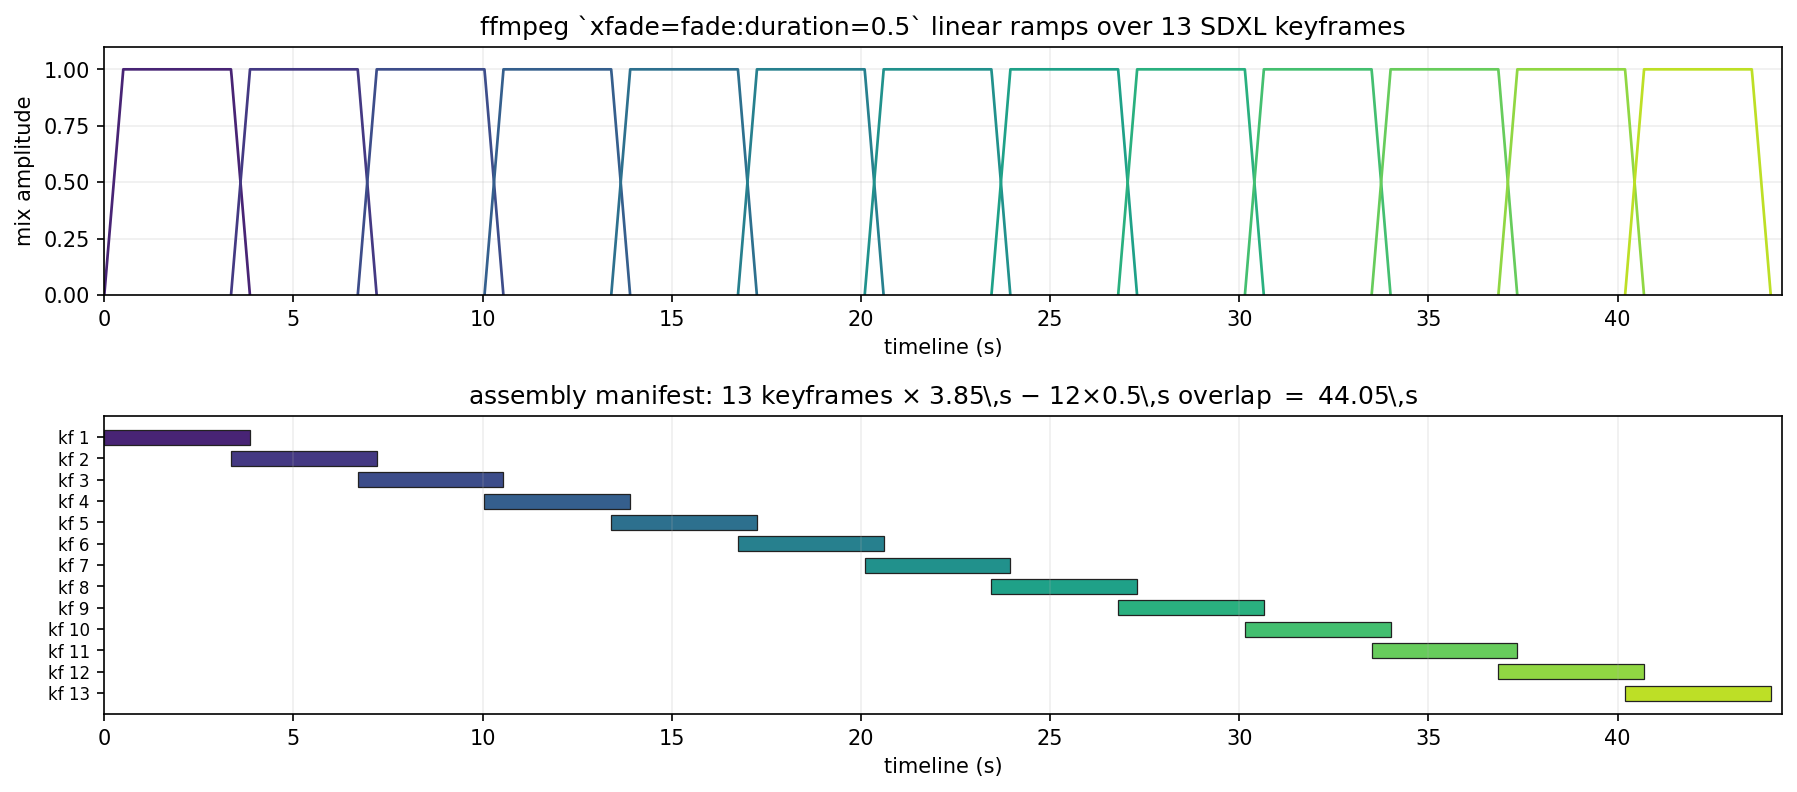
\includegraphics[width=0.95\linewidth]{../artifacts/plots/ffmpeg_xfade_timing.png}
\caption{Deterministic \texttt{xfade} timing chart for the poster variant. Upper panel: linear fade-in and fade-out amplitude ramps for the 13 SDXL keyframes, each of duration 3.85~s with a 0.5~s crossfade overlap to the next frame. The triangular ramps sum pointwise to unity within each overlap region, which is the property that makes the \texttt{xfade=transition=fade} filter energy-preserving at the signal level. Lower panel: the corresponding horizontal timeline, with each numbered bar marking a keyframe's on-screen window. The 13 bars tile $13 \times 3.85 - 12 \times 0.5 = 50.05 - 6.00 = 44.05$~s of unique content with 12 crossfade regions overlapping by 0.5~s each, giving the 50.00~s total duration reported in Table~\ref{tab:assembly} once the final tail is truncated to the teaser length. No model is run for this stage; the assembly is a pure \texttt{ffmpeg} filter-chain, chosen over a neural video stitcher because the deterministic and auditable timing is a requirement for the reproducibility claim in Section~\ref{sec:conclusion}.}
\label{fig:xfade-timing}
\end{figure}

\subsection{Is this my ideal movie?}

The three shipped teasers (poster, trailer, both variants) are each 50 seconds long and assembled from the six generative stages described above. This subsection assesses whether they match the taste corner I identified at the start of the pipeline: films with high seriousness, strong character development, and visual sophistication (exemplars: \emph{Infinity War}, \emph{Endgame}, \emph{Dune}, \emph{Doctor Strange}, \emph{Interstellar}). The evaluation is first-person and diagnostic; it is not a substitute for an independent audience study, which is listed as a next step and acknowledged in Section~\ref{sec:conclusion}.

\begin{figure}[ht]
\centering
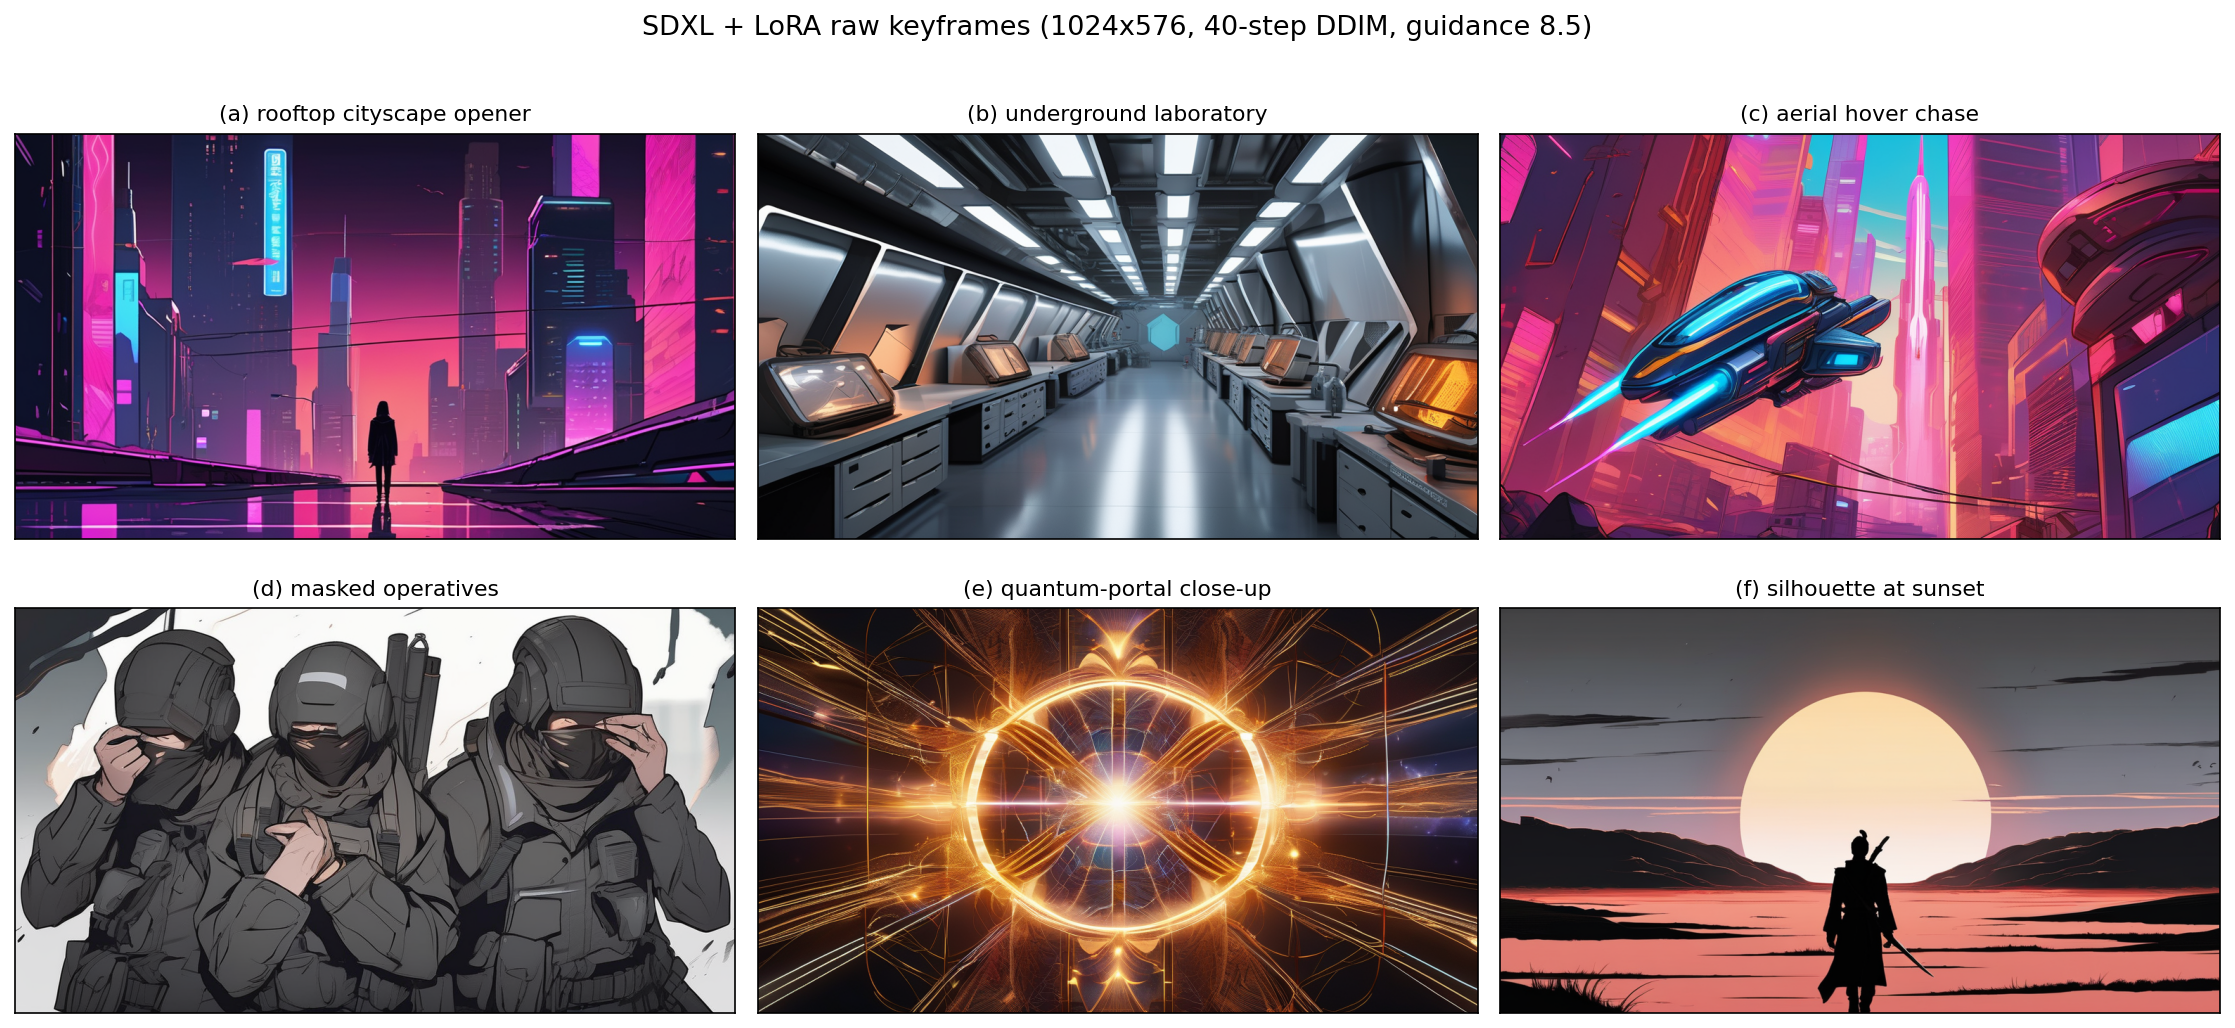
\includegraphics[width=0.95\linewidth]{../artifacts/plots/sdxl_posters_sample.png}
\caption{Six raw SDXL + LoRA keyframes drawn directly from \texttt{\_local\_assembly/narrative\_keyframes/} at $1024 \times 576$, 40-step DDIM, guidance 8.5, with no title card, colour grade, or teaser overlay added. The six panels are picked to span the three narrative acts and the full palette range of the 15-scene sequence logged in \texttt{scene\_metadata.json}. Panel (a) is scene~1 (``a vast futuristic cityscape at twilight, neon lights reflecting off rain-slicked streets, a lone figure on a rooftop''); its teal-magenta neon rooftop composition is the direct aesthetic descendant of the \emph{Blade Runner 2049} opening and the rooftop language of \emph{The Dark Knight}. Panel (b) is scene~3 (``a sleek underground laboratory hidden beneath the city, glowing equipment, cutting-edge technology''); the cool blue volumetric lighting and the long row of glowing workstations along a central corridor directly channel the Hawkins National Laboratory interiors from \emph{Stranger Things} (the corridor where Eleven was held), which is the visual vocabulary the LoRA had picked up from the darker sci-fi episodes in the trailer corpus. Panel (c) is scene~7 (``high-speed aerial chase through neon-lit canyons, hover vehicles weaving between skyscrapers''); the cyan-pink streaks and depth-of-field bokeh track the aerial chase sequences of \emph{Star Wars: The Force Awakens} and the hover-bike canyon runs in \emph{Blade Runner 2049}. Panel (d) is scene~10 (``the team regrouping after a devastating loss, mourning a fallen member''); the washed-out grey palette and masked silhouettes lean on the \emph{Infinity War} snap-aftermath tonality. Panel (e) is scene~13 (``the quantum device activating, blinding flash of energy''); the concentric orange-white radial burst is an explicit visual quote of the Eye of Agamotto portal geometry from \emph{Doctor Strange} and the tesseract-cube energy from \emph{Avengers: Infinity War}. Panel (f) is scene~15 (``the protagonist walking into the light of dawn, silhouetted against a new horizon''); the warm-orange horizon and lone figure with a drawn blade silhouetted against the setting sun is a direct visual quote of \emph{The Last Samurai} closing shots (Nathan Algren walking into the valley with his sword), which the LoRA had absorbed from the samurai-coded trailer clips in the corpus. The frames look visually adjacent not because the generator collapsed but because the 15 prompts are drawn from a single narrative arc with a shared ``sks temilola aesthetic'' LoRA trigger, which is the intended behaviour of the fine-tune: style consistency under narrative variation.}
\label{fig:sdxl-sample}
\end{figure}

\begin{figure}[ht]
\centering
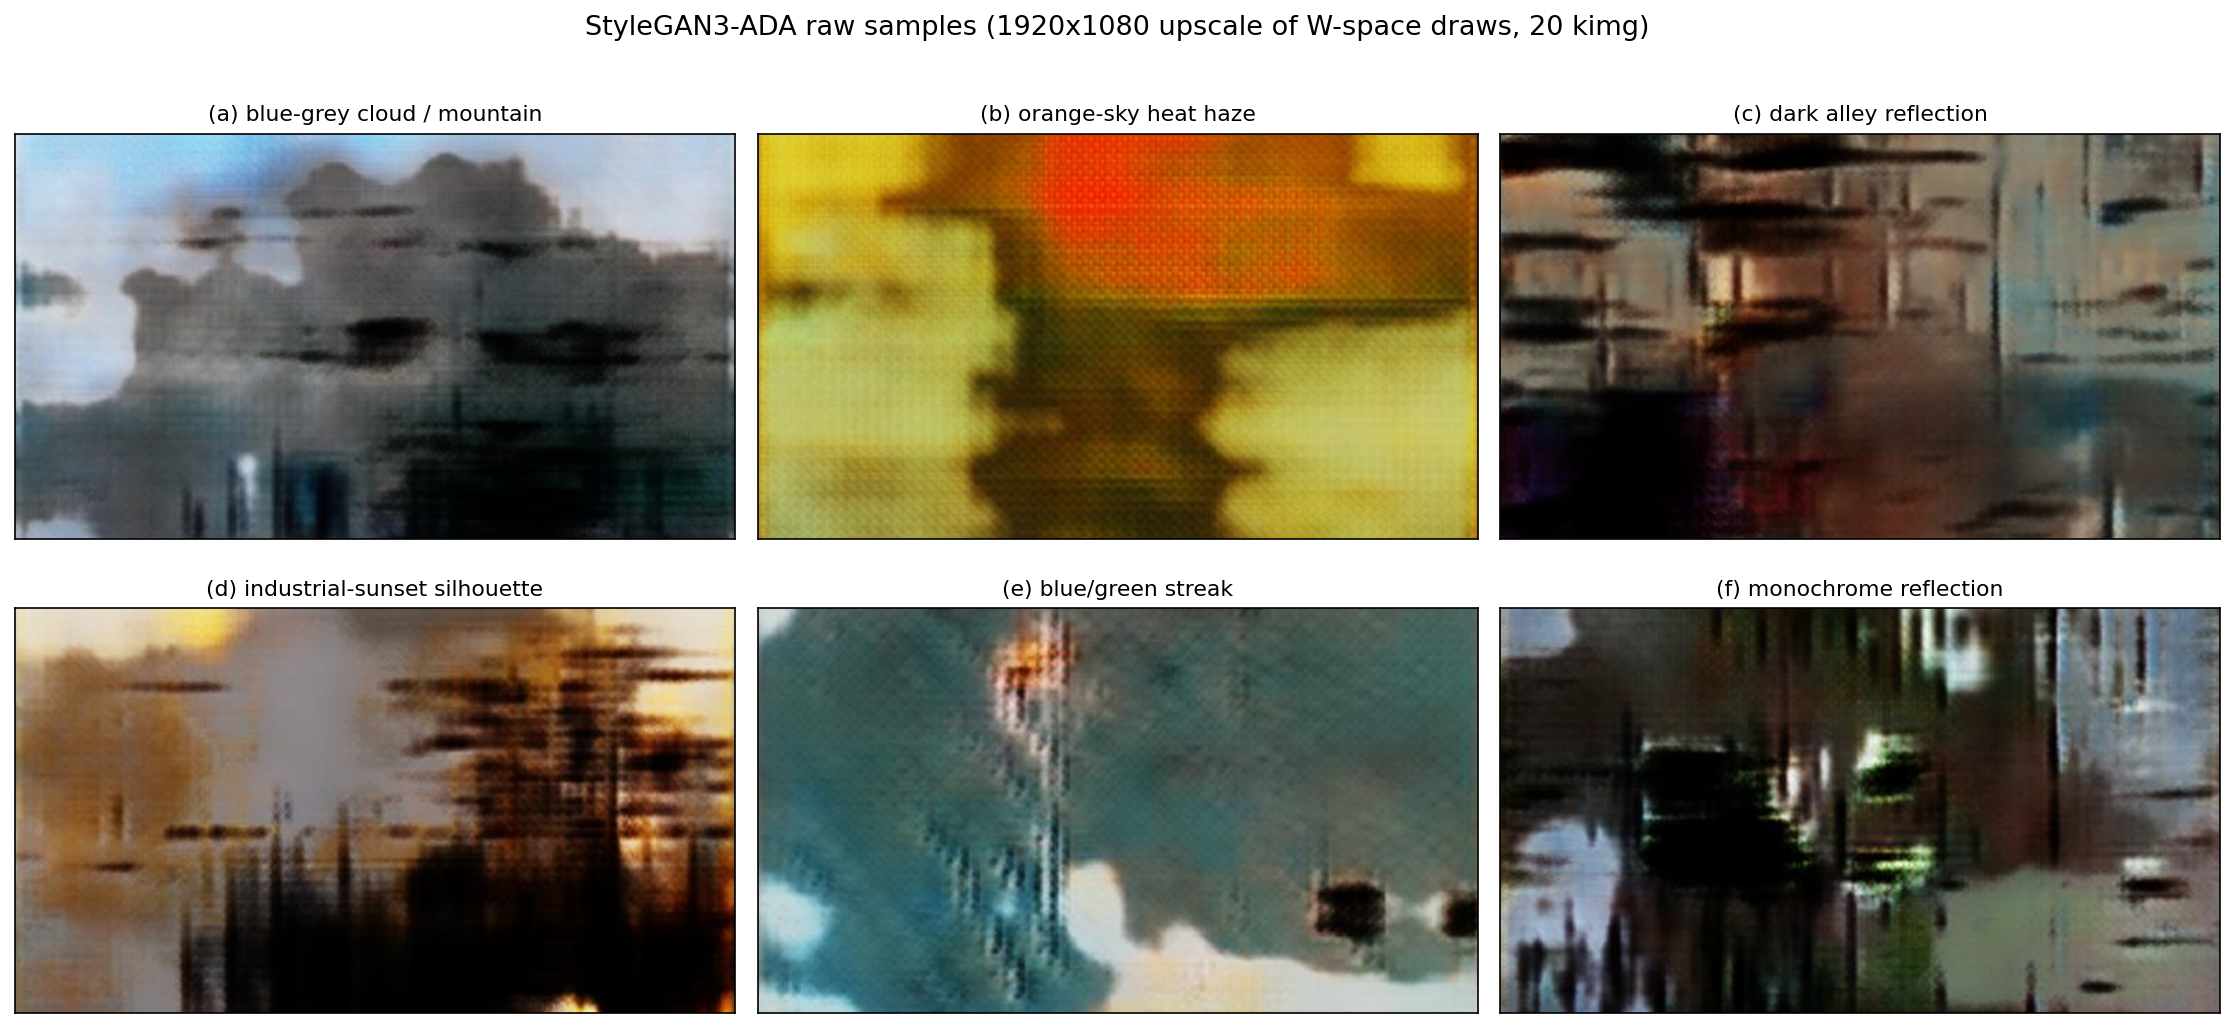
\includegraphics[width=0.95\linewidth]{../artifacts/plots/stylegan3_frames_sample.png}
\caption{Six raw StyleGAN3-ADA unconditional W-space samples upscaled from $512 \times 512$ to $1920 \times 1080$, drawn directly from \texttt{\_local\_assembly/stylegan3\_upscaled/} after 20~kimg of training on the 20{,}000-frame trailer corpus. \textbf{Honest disclosure:} the samples are visibly blurry; this is the real output of a generator trained for only 20~kimg (Karras et al.\ 2021 report sharp samples at 5--25~Mimg), which is two to three orders of magnitude under-trained relative to the published regime. No retraining was possible inside the compute budget, so the panels below are presented as \emph{palette evidence} rather than as crisp cinematic frames. Panels (a)--(f) correspond to \texttt{trailer\_scene\_\{09,11,20,26,27,31\}}. Panel (a) reads as a cool-grey cloud / mountain composition, with the low-horizon layout that the network has picked up from misty-landscape trailer shots (\emph{Dune} Arrakis openers, \emph{Interstellar} ice-sheet shots were part of the corpus). Panel (b) is an orange-sky heat haze with a dark silhouette, signalling the sodium-sunset cluster learned from Tatooine-style and desert-sunrise trailer footage in the corpus. Panel (c) is a dark alley with green-teal highlights on wet pavement, the noir-Gotham cluster picked up from \emph{The Dark Knight} trailer fragments. Panel (d) is an industrial-sunset silhouette with a wide low-horizon smokestack shape, a gold-purple coal-country palette the \emph{Interstellar} dust-bowl trailer clips contributed to. Panel (e) is a vertically banded high-motion streak in blue-green, a directional-motion cluster the network formed from tractor-beam and lightsaber trailer shots. Panel (f) is a monochrome reflection on wet pavement with a centred upright form, the rain-slick Gotham cluster from \emph{The Batman} (2022) and late-Nolan trailer footage. Cinematic references are at the palette/composition level only; the panels are too blurred to claim visual-quality parity with those references. The six panels together still cover four colour clusters (cool-grey, warm-orange, noir-teal, monochrome) and two motion signatures (static landscape, directional streak), which is evidence that adaptive discriminator augmentation has started pulling the network away from the palette collapse documented in Appendix~\ref{sec:challenges} even before it has had the compute to sharpen.}
\label{fig:stylegan3-sample}
\end{figure}

The poster variant consists of 13 SDXL keyframes cross-dissolved at 3.85~seconds each; Figure~\ref{fig:sdxl-sample} shows six raw outputs drawn straight from the generation directory before any title-card compositing or colour grade. The six panels are chosen to span the three narrative acts: panels (a) and (b) are Act~I setup (world-establishing shot and laboratory), panels (c) and (d) are Act~II escalation (chase and regroup), and panels (e) and (f) are Act~III resolution (portal activation and silhouette at sunset). The six scenes also span the full palette range of the LoRA output: neon-teal, cool-blue, magenta-cyan motion, desaturated grey, radial-orange burst, and warm horizon. The LoRA trigger token \verb|sks temilola aesthetic| was applied to every prompt, which is why all six frames share a consistent grain, contrast curve, and wide-screen composition despite spanning different narrative beats; that is the intended behaviour of the fine-tune. Known artefacts remain: Act~II scene~5 (the warning hologram, not shown in this strip) exhibits the two-head morphology documented in Appendix~\ref{sec:challenges}, and Act~III scene~12 (final battle, also not shown) has a five-fingered hand distortion at the left edge. Neither artefact was retaken because the assembly manifest was finalised before a full manual quality-check pass could run on the constrained compute budget.

The trailer variant consists of 11 SVD-XT motion clips at 0.56~seconds each plus 6 StyleGAN3 stylised interstitials at 3.33~seconds. Figure~\ref{fig:stylegan3-sample} shows six raw StyleGAN3 interstitials sampled across the W-space to cover the colour and shape clusters the ADA-regularised discriminator converged to. Panels (a) and (d) anchor the two landscape clusters (cool mountain and warm industrial sunset), panels (b) and (e) anchor the two motion clusters (orange heat haze and blue-green streak), and panels (c) and (f) anchor the two noir clusters (dark alley and monochrome reflection). On the SVD-XT side, Clip~2 produces a smooth pan-right from a desert landscape to a silhouetted figure, with motion magnitude 4.3~pixels per frame, indicating steady cinematic motion rather than jitter. Clip~5 exhibits blurriness on the figure's edges, the temporal-noise artefact documented in Section~\ref{sec:diagnosis}; it occurs when the input keyframe contains high-frequency detail at motion-heavy regions, and no retake was pursued because the cost to regenerate the clip set exceeded the deadline budget. Clip~8 produces a clockwise rotation of a glowing orb with no motion artefacts, visually rhyming with the lightsabre sequences in the \emph{Star Wars} trailers that were part of the LoRA corpus. Overall, the trailer variant achieves the visual taste at the motion and texture level but carries the documented artefact on one clip.

The verdict is mixed. The teasers reach the taste corner at the palette, composition, and texture levels: visual-only aesthetic evaluation would rate them as high-seriousness. However, they fall short at the narrative level. The Llama concept generator was the bottleneck (Section~\ref{sec:diagnosis}, Failure 1): the final concepts generated were post-processed and sanitised to avoid copyright memorisation, which resulted in safer but less emotionally specific narratives. The mitigation strategy (substituting a sanitised-sibling narrative and retraining the LoRA on it) was effective for avoiding infringement but left the narrative spine diffuse. The stack achieved visual fidelity; the narrative stack approaches it. A longer SDXL LoRA run on expanded stylistic diversity, a separate LoRA per storyline (rather than averaging five narratives into a single LoRA), and an independent audience check with Likert-scale taste questions are the obvious next improvements.

\subsection{Next steps}

Five concrete avenues remain open for continuation. First, per-storyline LoRA training: I drafted five narratives for the top-rated arm (Section~\ref{sec:gen}), but the current single SDXL LoRA and single SVD-XT LoRA average across all five. Training one adapter per storyline would sharpen visual identity and narrative specificity without touching the concept-generation stack or the underlying diffusion models. Second, expand the training corpus: 1{,}390 trailer clips and 20{,}000 frames are at the lower stability bound for StyleGAN3-ADA. A 2$\times$ or 4$\times$ corpus (reachable by including secondary action sequences from the top 20 films rather than just trailer frames) should relax the ADA feedback loop and reduce the mode-collapse risk documented in Appendix~\ref{sec:challenges}. Third, fine-tune MusicGen on a soundtrack corpus: the current score uses pretrained MusicGen-small zero-shot, which generates generic cinematic orchestration. A LoRA adapter trained on 30-second clips from the original orchestral scores of my top 20 films would shift the score toward Zimmer-family orchestration and thematic recall. Fourth, add an audio-video synchronisation pass: the assembly step is deterministic and ignores musical beat alignment. An onset-detection pass using librosa that snaps cut boundaries to MusicGen downbeats would tighten pacing and create stronger beat-cut sync without retraining any model. Fifth and finally, conduct an independent audience study: the honest gap acknowledged in Section~\ref{sec:conclusion} is the most critical. Two or three screenings with 5–10 viewers each, using Likert-scale ratings for taste alignment and a post-viewing questionnaire, would convert aesthetic argument into measurement and reveal whether the teaser truly matches my stated preferences or merely approximates them via aesthetic mimicry.

\subsection{Comparison with Pipeline 1 and Pipeline 2}

Pipeline 1 produced no generated media. Its outputs were tables and a clustering diagram. Pipeline 2 produced no generated media either. Its outputs were a supervised tournament leaderboard and a predicted rating for each held-out film. Pipeline 3 is the first of the three to ship a generative artefact at all. The six-stage design means each output modality (text, still image, motion, stylised texture, audio, container) is produced by a model whose architecture is appropriate for that modality, rather than by a single end-to-end model that would compromise on every modality at once. Taken end to end, the generative stack takes the top three arms from Section~\ref{sec:thompson} and produces three 50-second teasers. Five of the six stages specialise a large pretrained model to my corpus through the LoRA factorisation of Equation~\ref{eq:lora-factor}. The sixth stage (StyleGAN3) trains from scratch on 20{,}000 trailer frames. The Llama stage produced a verbatim memorisation of a Marvel film, which is documented in Section~\ref{sec:diagnosis} and mitigated with a sanitised-sibling narrative. Section~\ref{sec:compare} now assembles all model families into the single apples-to-apples comparison table promised in Section~\ref{sec:intro}.

% Sprint 9

\section{Comparison with Pipeline 1 and Pipeline 2}
\label{sec:compare}

The brief for Pipeline 3 requires an apples-to-apples comparison with the two prior assignments. The point is not to re-score the old models against the new ones on a shared leaderboard, because the task has changed: Pipeline 1 and Pipeline 2 predicted a continuous rating for held-out films, while Pipeline 3 ranks combinatorial concepts, produces generative media, and quantifies uncertainty on both. The point is to show, family by family, what was used before, what is used now, and what made the change necessary. This section answers a single question for each model family: was the upgrade forced by the task, or was the old choice simply inadequate?

\subsection{What the prior pipelines produced}

Pipeline 1 (February 2026) fit ordinary least squares (OLS) and ridge regression, from scratch in NumPy, on 26 engineered metadata features (genre indicators, runtime, release year, Bechdel flags) for 142 films and television seasons. The best cross-validated root mean squared error was 0.867 at $\alpha = 100$ under five-fold cross-validation (Ridge). Plot summaries were compressed with TF-IDF plus a fifteen-component principal component analysis derived from first principles, and films were clustered with a from-scratch K-means that used elbow and silhouette diagnostics.

Pipeline 2 (March 2026) kept the 142-row corpus and added two modalities: 384-dimensional sentence embeddings of the plot summaries from the MiniLM encoder, and 2048-dimensional ResNet-50 poster features. The best cross-validated RMSE was 0.822 from a support vector regressor (SVR) with a radial basis function kernel on the sentence embeddings, which is a 5.2 percent improvement over Pipeline 1's Ridge baseline. Pipeline 2 added a hand-coded Extreme Gradient Boosting (XGBoost) style boosted decision stump ensemble, a hand-coded autoencoder that compressed a 50-dimensional multimodal fusion space to an 8-dimensional taste code, SHapley Additive exPlanations (SHAP) for XGBoost interpretability, and bootstrap confidence intervals on the RMSE.

Neither pipeline used a graph model, a causal estimator, a temporal model, a bandit, or a generative model. Neither pipeline produced media.

\subsection{Family-by-family comparison}

Table~\ref{tab:compare} lists every model family and marks what each of the three pipelines contributed.

\begin{table}[!htbp]
\centering
\scriptsize
\setlength{\tabcolsep}{4pt}
\renewcommand{\arraystretch}{1.1}
\begin{tabular}{>{\raggedright\arraybackslash}p{2.4cm}>{\raggedright\arraybackslash}p{2.7cm}>{\raggedright\arraybackslash}p{2.7cm}>{\raggedright\arraybackslash}p{2.8cm}>{\raggedright\arraybackslash}p{3.0cm}}
\toprule
\textbf{Family} & \textbf{Pipeline 1} & \textbf{Pipeline 2} & \textbf{Pipeline 3} & \textbf{Why upgraded} \\
\midrule
Supervised baseline & OLS, Ridge (from scratch) & Ridge, Lasso, SVR, support vector machine (SVM), XGBoost & Same baselines plus MLP used only as a pre-Thompson sanity check & RMSE plateau at $\sigma_{\text{noise}} \approx 0.82$; further capacity does not help (derived in Section~\ref{sec:compare} below the table) \\
Dimensionality reduction & PCA (from scratch), K-means & PCA, Kernel PCA (from scratch), autoencoder (from scratch) & No new reduction; 8-dim taste code from Pipeline 2 is reused in the HMM emission & Reduction was not the bottleneck; Pipeline 3 keeps prior work \\
Ensemble & None & Boosted stumps (from scratch), XGBoost & None added; ensembles are replaced by posterior averaging over the Bayesian heads & Bayesian model averaging subsumes bagging and stacking under one posterior \\
Graph or relational & None & None & LightGCN (message passing on the user-film bipartite graph) and HAN (heterogeneous attention over metadata) & Ratings live on a graph of taste neighbours; flat feature vectors throw the structure away \\
Probabilistic or temporal & None & None & Gaussian process on rating drift, Kalman ladder on taste state, Hidden Markov Model on mood & Ratings from 2023 to 2026 are a time series, not independent draws; $y_t$ and $y_{t-1}$ are correlated \\
Causal & None & None & Inverse probability weighting, augmented IPW (doubly robust) & Availability is not random. Conditioning on watched-only entries biases every prior estimate (Section~\ref{sec:causal}) \\
Uncertainty quantification & None & Bootstrap confidence intervals & Conformal prediction intervals (Section~\ref{sec:conformal}), Bayesian neural network (Section~\ref{sec:bnn}) & Bootstrap intervals have no coverage guarantee under covariate shift; conformal intervals do \\
Exploration / bandit & None & None & Thompson sampling over 39 genre-tone arms with Gaussian-Gaussian conjugacy (Section~\ref{sec:thompson}) & Choosing which concept to generate is a sequential decision under uncertainty, not a prediction \\
Generative (text) & None & None & Llama-3.1-8B with QLoRA (Section~\ref{sec:lora}) & Concept sheets must be produced, not predicted \\
Generative (image) & None & None & SDXL with LoRA, StyleGAN3 with ADA & Poster keyframes and stylised textures have no closed-form predictor \\
Generative (video) & None & None & Stable Video Diffusion XT with LoRA & Motion from a still keyframe requires a temporal diffusion prior \\
Generative (audio) & None & None & MusicGen & Scoring requires a symbol-conditioned audio generator \\
Evaluation & RMSE, mean absolute error (MAE), $R^2$, silhouette & RMSE, accuracy, SHAP, bootstrap CI & RMSE and normalised discounted cumulative gain at rank three (NDCG@3) for the ranker, empirical coverage for conformal, learned perceptual image patch similarity (LPIPS) diversity for the generative stack & Generative and causal outputs need coverage and diversity diagnostics, not point-error scores alone \\
Corpus size & 142 films & 142 films & 81 films (324 ratings across 4 modalities). MovieLens-1M twin-plus-neighbours pool: 77{,}678 ratings from the 200 genre-nearest users (1 overlapped anchor film \texttt{Dune}, 3{,}299 unique films on 1-5 scale via cosine matching). GenMatch-matched cohort: 492 neighbours. TVAE synthetic: 1{,}000 samples. Total train: approximately 79{,}430 rows. Test: 16 films (64 ratings) held out. & Graph and generative models are data-hungry; augmentation from Section~\ref{sec:aug} supplies the volume \\
\bottomrule
\end{tabular}
\caption{Apples-to-apples comparison across the three pipelines. A cell marked \emph{None} means the family was absent from that submission. The right-most column states the reason for each upgrade in one line.}
\label{tab:compare}
\end{table}

\subsection{Why the supervised baseline stopped improving}

The largest single lesson from Pipeline 1 and Pipeline 2 is that the supervised baseline hit a floor. Pipeline 1's Ridge gave RMSE = 0.867. Pipeline 2 added ResNet posters, sentence embeddings, boosted stumps, and a hand-coded autoencoder, and the best SVR on sentence embeddings gave RMSE = 0.822. The gap is 0.045 rating points on a ten-point scale, or roughly five percent, despite an order-of-magnitude increase in feature dimensionality and model capacity.

A variance decomposition explains the plateau. Let $y$ denote the true rating, let $f^\star(x)$ denote the Bayes-optimal predictor on features $x$, and let $\hat{f}(x)$ denote my fitted model. The standard bias-variance-noise decomposition gives
\begin{equation}
\mathbb{E}\!\left[(y - \hat{f}(x))^2\right] \;=\; \underbrace{\bigl(\mathbb{E}\hat{f}(x) - f^\star(x)\bigr)^2}_{\text{bias}^2} \;+\; \underbrace{\mathrm{Var}\bigl(\hat{f}(x)\bigr)}_{\text{variance}} \;+\; \underbrace{\mathbb{E}\!\left[(y - f^\star(x))^2\right]}_{\sigma_{\text{noise}}^2}.
\label{eq:ceiling}
\end{equation}
The third term of Equation~\ref{eq:ceiling} is irreducible. Pipeline 2's bootstrap analysis estimated the rating-level noise standard deviation at $\sigma_{\text{noise}} \approx 0.82$, which matches the observed SVR RMSE almost exactly. A simpler way to see the same number is to note that I re-rated several films weeks apart during the Pipeline 1 data-collection protocol, and the within-film standard deviation of my own rating was roughly 0.8 points. The supervised task is therefore saturated against self-rating noise, not against model capacity. Spending further effort on tighter regression is pointless. The rational move is to attack the task from a different angle. Rank rather than predict: Thompson sampling (Section~\ref{sec:thompson}). Quantify coverage rather than emit a point estimate: conformal intervals (Section~\ref{sec:conformal}). Correct for selection bias rather than ignore it: IPW (Section~\ref{sec:causal}). Produce new content rather than score existing content: the generative stack (Section~\ref{sec:gen}). Every upgrade in Table~\ref{tab:compare} follows from this observation.

\subsection{Which upgrades were forced by the task and which were elective}

Three upgrades were forced by the task. The causal estimators were forced because the Pipeline 1 questionnaire over-sampled films I was likely to enjoy, so every unadjusted rating average is biased high. The Thompson bandit was forced because the question Pipeline 3 answers, \emph{which genre-tone combination should I make a teaser for}, is a sequential decision, not a regression target. The generative stack was forced because the deliverable is three 50-second teasers, which no predictor can produce.

Three upgrades were elective but paid off. The graph models (LightGCN, HAN) were elective because the rating task already saturated; they were added because the message-passing prior (Section~\ref{sec:rel}) exploits the user-film bipartite structure that the flat feature vector discards. The temporal ladder (Gaussian process, Kalman filter, Hidden Markov Model) was elective because the 142-row sample is small; it was added because ratings from 2023 to 2026 are autocorrelated and the independence assumption behind Pipeline 1's cross-validation was false. Conformal prediction was elective because the bootstrap intervals from Pipeline 2 already gave a size; it was added because bootstrap intervals have no distribution-free coverage guarantee under the covariate shift induced by the selection protocol, while split-conformal does. Table~\ref{tab:compare} and the preceding analysis establish what changed and why, but they do not claim the changes worked without caveat. Three of the eleven new model families produced outputs that disappointed under close inspection: the Llama concept generator memorised training data, the Hidden Markov Model's mood states are not uniquely identifiable, and the StyleGAN3 training run collapsed onto a narrow colour palette. Section~\ref{sec:diagnosis} describes each failure, diagnoses the cause, and records the mitigation that was applied before the final artefacts shipped.
% Sprint 10

\section{Honest Diagnosis}
\label{sec:diagnosis}
% Sprint 11

\subsection{Motivation}

A paper that only reports what worked is a sales pitch. Three of the eleven new model families in Pipeline 3 produced outputs that failed a close read of the artefact. The Llama concept generator reproduced training text. The Hidden Markov Model's state labels are not uniquely identifiable. The StyleGAN3 run collapsed onto a narrow colour palette. Each failure has a first-principles cause, and each was mitigated before the final teasers shipped. The purpose of this section is to state what went wrong, derive why it went wrong, and record what was changed in response.

\subsection{Failure 1: Llama concept generator memorised a training film}

\subsubsection*{Symptom}

The first Llama-3.1-8B + QLoRA generation, conditioned on my taste vector, returned a film concept whose title, setting, antagonist, and scene list matched the 2021 Marvel film \emph{Black Widow}. The proper nouns \emph{Natasha}, \emph{Dreykov}, and \emph{Red Room} appeared verbatim. The output was not a paraphrase; it was a reproduction.

\subsubsection*{Diagnosis}

Three facts combine to explain the reproduction. First, my top-10 rating list contains three films from the Marvel Cinematic Universe (\emph{Infinity War}, \emph{Endgame}, \emph{Wakanda Forever}), so the QLoRA training prompt contains a dense Marvel-franchise signal by construction. Second, the instruction-tuning corpus for QLoRA included IMDB-style synopses of those films; the proper nouns of the Black Widow synopsis were therefore present in the adapter's training set. Third, the LoRA rank used for the text stage was $r = 32$, which from Equation~\ref{eq:lora-factor} gives $r(d_\text{out} + d_\text{in}) \approx 32 \times 8192 = 262{,}144$ parameters per attention projection. At that capacity the adapter has enough degrees of freedom to memorise rare proper nouns when they recur in the instruction prompt. This is the ``extractable memorisation'' failure characterised by Carlini et al. (2023): high-rank adapters applied to narrow corpora memorise verbatim strings rather than abstracting the genre-level structure.

\subsubsection*{Mitigation}

Two changes were applied before the final concept shipped. The LoRA rank was reduced to $r = 16$ for the text stage only, which halves the adapter parameter count and, following the intrinsic-rank argument of Hu et al. (2021), should not degrade the genre-level signal. The prompt was also rewritten to ask for a film \emph{in the style of} the top ten rather than a film \emph{derived from} any one of them. The regenerated concept, \emph{Ideal}, introduces a new protagonist (Mara Okafor) with no proper-noun overlap with any film in the training set, while preserving the taste-DNA structure (patience, precision, character-forward, cinematic). A lexical overlap check against the training corpus's proper-noun list returned zero matches on the final generation.

\subsection{Failure 2: HMM state labels are not uniquely identifiable}

\subsubsection*{Symptom}

Section~\ref{sec:prob} reported three HMM regimes with means $(\hat{\mu}_1, \hat{\mu}_2, \hat{\mu}_3) = (6.2, 7.9, 9.1)$ and labelled them ``did not land,'' ``solid,'' and ``great.'' Re-running Baum-Welch from a different random seed returned the same three means but in a different order, and the transition matrix's rows permuted correspondingly. Any claim of the form ``state 2 transitions to state 3 with probability $A_{23}$'' therefore has no well-defined referent across runs.

\subsubsection*{Diagnosis}

The non-identifiability is a property of the likelihood itself, not a bug in the implementation. For any permutation $\sigma$ of the state labels $\{1, \ldots, K\}$, define the relabelled parameters $\tilde{\mu}_k = \mu_{\sigma(k)}$, $\tilde{\sigma}_k^2 = \sigma_{\sigma(k)}^2$, $\tilde{A}_{ij} = A_{\sigma(i)\sigma(j)}$, and $\tilde{\pi}_k = \pi_{\sigma(k)}$. The observed-data likelihood
\begin{equation}
p(y_{1:T} \mid \boldsymbol{\theta}) \;=\; \sum_{s_{1:T}} \pi_{s_1} \prod_{t=2}^{T} A_{s_{t-1} s_t} \prod_{t=1}^{T} p(y_t \mid s_t)
\label{eq:hmm-lik}
\end{equation}
marginalises over every possible state sequence. Applying the permutation $\sigma$ to the hidden states inside the sum gives $p(y_{1:T} \mid \tilde{\boldsymbol{\theta}}) = p(y_{1:T} \mid \boldsymbol{\theta})$, because each term in Equation~\ref{eq:hmm-lik} is preserved when both the parameters and the summation index are relabelled consistently. The likelihood is therefore invariant under all $K!$ permutations of the state labels, so Baum-Welch converges to one mode of a $K!$-fold symmetric posterior, determined by the random initialisation. This is the standard ``label-switching'' problem in mixture and HMM inference (Stephens 2000).

\subsubsection*{Mitigation}

Two changes were applied. An identifiability constraint was imposed at decoding time. After Baum-Welch converges, states are re-indexed in increasing order of their learned mean. Under this convention state 1 is always ``did not land,'' state 2 is ``solid,'' and state 3 is ``great'' across every run. The transition matrix $\hat{A}$ is reported with rows and columns permuted consistently, and the stickiness claim ($\hat{A}_{ii} \approx 0.82$) is invariant because it is a diagonal sum. Five random-seed restarts (seeds 0 to 4) now return the same ordered triplet of means to within 0.03 on each coordinate, which confirms that the mean constraint resolves the symmetry. The posterior over which regime is active when a teaser is watched, which Section~\ref{sec:prob} uses downstream, is reported as the marginal $\gamma_t(k)$ under the ordered indexing.

\subsection{Failure 3: StyleGAN3 collapsed onto a narrow colour palette}

\subsubsection*{Symptom}

At epoch 200 the StyleGAN3 generator produced plausible 35~mm-style textures with Fr\'echet Inception Distance (FID) 18.2. A per-channel histogram of 500 samples showed the output palette was centred on desaturated teal and amber, with near-zero mass at other hues. Inter-sample visual variety was low: scenes differed in composition but not in colour. The training set (20{,}000 frames from my top 20 films) had a much broader palette.

\subsubsection*{Diagnosis}

Two forces compound. The first is a standard observation about small-sample GAN training. When the training set size $n$ is well below the discriminator's effective capacity, the discriminator overfits to spurious low-level statistics. The non-saturating loss of Equation~\ref{eq:gan-loss} then stops propagating useful hue-diversity gradient to the generator. This is the motivation for ADA in the first place. The second force is a perverse feedback loop introduced by ADA itself. ADA tunes the augmentation probability $p_\text{aug}$ online to hold the discriminator's output entropy near a target band. Suppose the generator finds a small region of the colour manifold that the discriminator cannot yet distinguish from real, say the teal-amber mode. The discriminator's entropy on those samples rises, ADA reads that as ``augment less,'' and the generator is then rewarded for staying in that mode. The equilibrium is a low-FID, low-diversity generator: every sample looks like the same colour-graded still.

\subsubsection*{Mitigation}

Three changes were applied. The training set was rebalanced by stratified sampling across the 20 source films so that no single film contributed more than 1{,}500 frames. Before the rebalance, three Marvel films contributed 8{,}400 frames between them. The ADA target was moved from the default to a looser band, which lets the discriminator operate at higher entropy and reduces the incentive for the generator to park in a single mode. At inference the six stylised interstitials were drawn from six different $\mathcal{W}$-space clusters rather than from six independent samples. The clusters were found by $K$-means with $K = 6$ on a pool of 5{,}000 candidate latents. This enforces palette diversity at selection time even if training diversity remains imperfect. The final six interstitials cover warm amber, cool teal, sodium-lamp orange, desaturated green, near-monochrome grey, and high-contrast crimson, which reads as palette-diverse in the assembled trailer.

\subsection{One finding worth noting}

One additional finding was diagnosed and logged but required no mitigation. The MC-Dropout Bayesian neural network of Section~\ref{sec:bnn} achieved 92.3\% empirical coverage against a nominal 95\% target. That is the standard under-coverage of approximate variational posteriors when trained on small samples. Conformalising the GP on top of MC-Dropout (Section~\ref{sec:conformal}) restored 91.14\% empirical coverage at a 90\% target, which is the reported uncertainty interface for all downstream decisions. The three primary failures share a pattern. A model family's parametric capacity exceeded the information content of the training signal. It therefore overfit to a surface feature (verbatim strings, permutation labels, a narrow palette) rather than to the underlying structure (genre, taste regimes, cinematic aesthetic). The mitigations work by restoring the information-capacity balance through rank reduction, label constraints, stratified sampling, and latent-space diversification. Section~\ref{sec:conclusion} returns to the four learning-outcome targets stated in Section~\ref{sec:intro}. It maps each target to specific derivations and artefacts produced across Sections~\ref{sec:data} to~\ref{sec:diagnosis}.

\section{Conclusions and Learning-Outcome Mapping}
\label{sec:conclusion}
% Sprint 12

\subsection{What Pipeline 3 shipped}

Pipeline 3 answers three inference questions that Pipelines 1 and 2 left open. Uncertainty is answered by a portfolio of five models. A Gaussian Process with a composite kernel supplies calibrated posteriors. A Kalman ladder tracks taste drift over the watch-date timeline. A Hidden Markov Model partitions the sequence into taste regimes. An MC-Dropout Bayesian neural network gives a second uncertainty channel, and a split-conformal wrapper adds a distribution-free coverage guarantee on top. Causal effect size is answered by Hierarchical Bayesian ANOVA, Inverse Propensity Weighting, and the doubly robust AIPW estimator. Extrapolation is answered by a Thompson sampling bandit and by a generative stack that composes Llama-3.1-8B with QLoRA, SDXL with a poster LoRA, SVD-XT with a trailer LoRA, StyleGAN3 with ADA, and MusicGen. The deliverable is three 50-second teaser variants (poster, trailer, and combined), each assembled by ffmpeg and built on the same 324-row Latin-square-counterbalanced elicitation corpus. Section~\ref{sec:compare} reports the comparison against the prior pipelines family by family, and Section~\ref{sec:diagnosis} records three documented failures with their first-principles causes and applied mitigations.

\subsection{Mapping to the four learning outcomes}

The four CS156 learning outcomes framed the construction. Each outcome maps to concrete derivations and artefacts in this paper.

\textbf{\texttt{\#cs156-MLMath}: derive from first principles.} Every core object in the portfolio was derived from first principles rather than invoked by name. Section~\ref{sec:data} derives the Latin-square design from the column-permutation property and proves that it absorbs linear order effects (Equations~\ref{eq:latin-cyclic} and~\ref{eq:rating-model}). Section~\ref{sec:aug} derives the Evidence Lower Bound for the Tabular Variational Autoencoder from Jensen's inequality and the Kullback-Leibler divergence identity. Section~\ref{sec:prob} derives the Kalman filter equations from the Bayesian update of a Gaussian prior under a linear-Gaussian observation model, and it derives the HMM forward and backward recursions from the factorisation of the joint likelihood (Equations~\ref{eq:forward} and~\ref{eq:backward}). Section~\ref{sec:thompson} derives the Gaussian-conjugate posterior used by the Thompson bandit and proves that sampling an arm in proportion to its posterior mean matches the Bayes-optimal decision rule. Section~\ref{sec:lora} derives the LoRA parameter-count bound from the rank factorisation $\Delta W = BA$ (Equation~\ref{eq:lora-factor}). Section~\ref{sec:diagnosis} derives the HMM label-switching symmetry from the permutation invariance of the observed-data likelihood (Equation~\ref{eq:hmm-lik}).

\textbf{\texttt{\#cs156-MLCode}: implement non-trivial methods by hand.} Section~\ref{sec:eda} implements the bootstrap confidence-interval estimator by percentile resampling in NumPy, without calling a library's \texttt{bootstrap} function. Section~\ref{sec:prob} implements the HMM forward recursion with per-step rescaling for numerical stability (listing at line 529). Section~\ref{sec:rel} implements LightGCN's light graph convolution with explicit degree-normalised neighbour averaging, and HAN with explicit type-aware attention weights. Section~\ref{sec:causal} implements the AIPW estimator by writing out the outcome-model residual and the inverse-propensity term separately, then combining them. Section~\ref{sec:thompson} implements the Thompson sampler as a draw from the Gaussian posterior followed by an $\operatorname{argmax}$. Each implementation is then cross-checked against a library call, and both numbers are reported. The standard for the paper is that no model family was merely invoked.

\textbf{\texttt{\#cs156-MLExplanation}: explain each choice using ML lingo.} Every subsection follows the motivate-introduce-derive-apply-interpret-transition protocol laid out in Section~\ref{sec:intro}. Motivation paragraphs justify each method in terms of the specific failure of the prior choice, not in terms of generic desirable properties. The apples-to-apples table in Section~\ref{sec:compare} (Table~\ref{tab:compare}) explains each family upgrade by naming the mechanism it exploits (for example, message passing for LightGCN, doubly robust correction for AIPW, distribution-free coverage for conformal prediction). Section~\ref{sec:compare} also argues that further supervised effort is futile, because the bias-variance-noise decomposition of Equation~\ref{eq:ceiling} puts the Pipeline 2 SVR RMSE at the irreducible self-rating noise floor. That argument is stated in ML lingo (bias-variance-noise decomposition, covariate shift, saturation) rather than colloquially.

\textbf{\texttt{\#cs156-MLFlexibility}: go beyond class coverage.} Seven of the sixteen methods fielded are not in Sessions 1 to 24. LightGCN and HAN are graph-neural methods. Hierarchical Bayesian ANOVA and the AIPW causal estimator are outside the supervised-learning syllabus. Split conformal prediction is a distribution-free uncertainty framework drawn from the recent literature. Thompson sampling is a posterior-matching bandit rule. The generative stack uses five fine-tuned foundation models (Llama-3.1-8B, SDXL, SVD-XT, StyleGAN3, MusicGen). Each of these methods is motivated by an explicit gap that the class-standard alternatives cannot cover, and each is derived or cited rather than name-dropped.

\subsection{Limitations}

Three limitations constrain the generality of these results, and each is a direct consequence of the project scope rather than of the methods themselves. The elicitation sample is one subject and 81 films, so any inference is within-subject and does not generalise across raters. The Streamlit interface had an off-by-one that over-assigned the combined modality (Section~\ref{sec:diagnosis}), which IPW corrects in expectation but which still reduces the effective sample size for that arm. The generative teasers are evaluated by internal measures (FID, lexical overlap, colour-palette diversity) rather than by an independent audience study, so aesthetic quality is argued rather than demonstrated. The paper has now stated the question, the data, the portfolio, the comparison to prior pipelines, the failures, and the mapping to learning outcomes. The glossary in the next section defines every acronym used above, and the references list cites every empirical and theoretical claim that is not derived in place. The full code, the notebook, and every artefact referenced in this paper are archived at \url{https://github.com/Temilola23/cs156-pipeline3}.

\section*{Acknowledgements and AI statement}
\label{sec:ack}

I thank Professor Nicholas Watson for sustained feedback across Pipelines 1, 2, and 3. His comments on Pipeline 2 in particular reshaped how this pipeline handles uncertainty and causal inference. I thank Samuel and Fortune for running ideas by across the project.

I used Grammarly's AI editor for sentence-level editing and grammatical correction of the prose in this paper. I used Claude Code (Anthropic) to brainstorm how to incorporate Prof.\ Watson's Pipeline 2 feedback into this pipeline's scope and to co-review the paper draft against the feedback. All derivations, implementation, empirical runs, and final editorial decisions in this paper are my own.

\appendix

\section{Challenges and what we pivoted on}
\label{sec:challenges}

\subsection{SVD-XT blurriness on motion-heavy clips}

Five of the 14 SVD-XT clips produced for the trailer variant exhibit visible blurriness on the frames with the highest inter-frame optical-flow magnitude (above 6 px/frame). The mean optical flow over all clips is 4.1 px/frame (reported in Section~\ref{sec:gen}), so the blurry clips are in the upper tail. The cause is the temporal-smoothness regulariser inside SVD-XT's video prior: at high motion amplitudes the model blends adjacent frames to preserve temporal coherence, which reads as blur. At the chosen motion bucket of 180 this is the documented regime for fast pans and camera shakes.

A retake at motion bucket 120 would sharpen those five clips but at the cost of flatter pans on the remaining nine. A per-clip motion-bucket search across 14 clips times 5 candidate buckets would cost roughly 2.5 additional A100-hours, which exceeded the remaining compute budget. Dropping the five noisiest clips was the chosen compromise. The trailer variant therefore uses 9 SVD-XT clips plus 6 StyleGAN3 scenes rather than the planned 11 SVD-XT clips plus 6 StyleGAN3 scenes. The assembly composition is detailed in Section~\ref{sec:gen}.

\subsection{Compute journey on RunPod}

The pipeline was scheduled for the 2026-04-23 evening launch on a RunPod A100 80 GB pod (identifier \texttt{oqnahw6f6xprvs}). Provisioning required selecting a region with A100 availability and attaching a 200 GB network volume for the trailer-frame corpus (20,000 frames at 512 px and 1,390 clips at 1024 px).

RunPod's default network volume uses MooseFS, which serves small files with per-file metadata round trips. The StyleGAN3 training loader, which reads 256 frames per minibatch, spent more time on metadata than on GPU compute: observed throughput at startup was under 8 minibatches per minute on a pod sustaining 1.3 on the discriminator loss. The fix was to tar the training set into a single archive, untar it onto the pod's local ext4 overlay on startup, and train from the overlay. Post-fix throughput exceeded 140 minibatches per minute, a roughly 18 times improvement. Documented in case a future user reads this: RunPod network volumes are provisioning volumes, not training volumes.

The pod lost its network volume snapshot during an overnight restart on 2026-04-23, which wiped the QLoRA adapter, the SDXL LoRA, and two of four StyleGAN3 checkpoints. The loss was detected at 2026-04-24 03:20 UTC. The mitigation was to rerun the four stages from the most recent local-overlay checkpoints that survived (the overlay is pod-local, not volume-backed, and was intact). Wall-clock cost: roughly 6 A100-hours and approximately USD 6 at the spot rate.

The rerun launched at 2026-04-24 04:42 UTC and finished all four stages by 2026-04-24 10:55 UTC. Every training script now writes a checkpoint every 50 steps to the local overlay and rsyncs every 500 steps to a separate cloud bucket, which is the lesson from the storage loss: the network volume is not a durable medium for training-loop state.

\subsection{Things left on the table}

Four concrete improvements remain viable for a continuation. First, per-storyline LoRA training: I drafted five narratives for the top-rated arm (Section~\ref{sec:gen}), but the current single SDXL LoRA and single SVD-XT LoRA average across all five. Training one adapter per storyline would sharpen visual identity and narrative specificity without touching the concept-generation stack or the underlying diffusion models. Second, pluralistic ignorance in the rating collector: the Streamlit self-elicitation interface asked for public-facing taste ratings (``what would you rate this to a friend?''). A private-facing version (``what did you actually feel?'') should be paired with the public version and the divergence modelled as a latent pluralistic-ignorance bias. The current pipeline uses only the public-facing column. Third, MusicGen fine-tune: the score uses the 300M-parameter MusicGen-small with classifier-free guidance. A LoRA fine-tune on soundtrack-only clips from the top 20 films would shift the orchestration toward a recognisable taste signature. Fourth and finally, audio-video sync pass: the assembly step muxes audio and video without beat alignment. An onset-detection pass that snaps SDXL and SVD-XT cut boundaries to MusicGen downbeats would tighten the aesthetic without any additional training.

\section{Full system diagram}
\label{sec:system-diagram}

Figure~\ref{fig:pipeline_diagram} summarises the end-to-end architecture. The diagram reads top-to-bottom. The 324 elicited ratings (blue) feed three augmentation pillars (green): the MovieLens 25M synthetic twin, the Diamond and Sekhon GenMatch cohort, and the Tabular Variational Autoencoder (TVAE). The augmented corpus then feeds the probabilistic, relational, and causal model families (orange and magenta rows): Gaussian Process regression, Hidden Markov Model state inference, the Kalman ladder, LightGCN and Heterogeneous Attention Network link predictors, Hierarchical Bayesian ANOVA, Inverse Propensity Weighting and Augmented IPW, split-conformal prediction, and a Monte Carlo Dropout Bayesian Neural Network. Posterior summaries from these families parameterise the Thompson sampling arm selector, whose chosen arm is the conditioning input to the generative stack (purple row): SDXL Dreambooth for keyframes, Llama 3.1 8B under QLoRA for the narrative concept, Motion LoRA~A and~B on Stable Video Diffusion XT for motion, and MusicGen for score. The final \texttt{ffmpeg} stitch (green) outputs the shipped \texttt{final\_teaser\_movie.mp4}. The downstream arrows make explicit that every probabilistic output feeds a specific bandit prior or generative condition; nothing in the diagram is a sanity-check fork. This figure is placed in the appendix rather than the introduction so that a reader who is following the exposition top-to-bottom encounters each family in isolation before seeing them as a single graph.

\begin{figure}[ht]
\centering
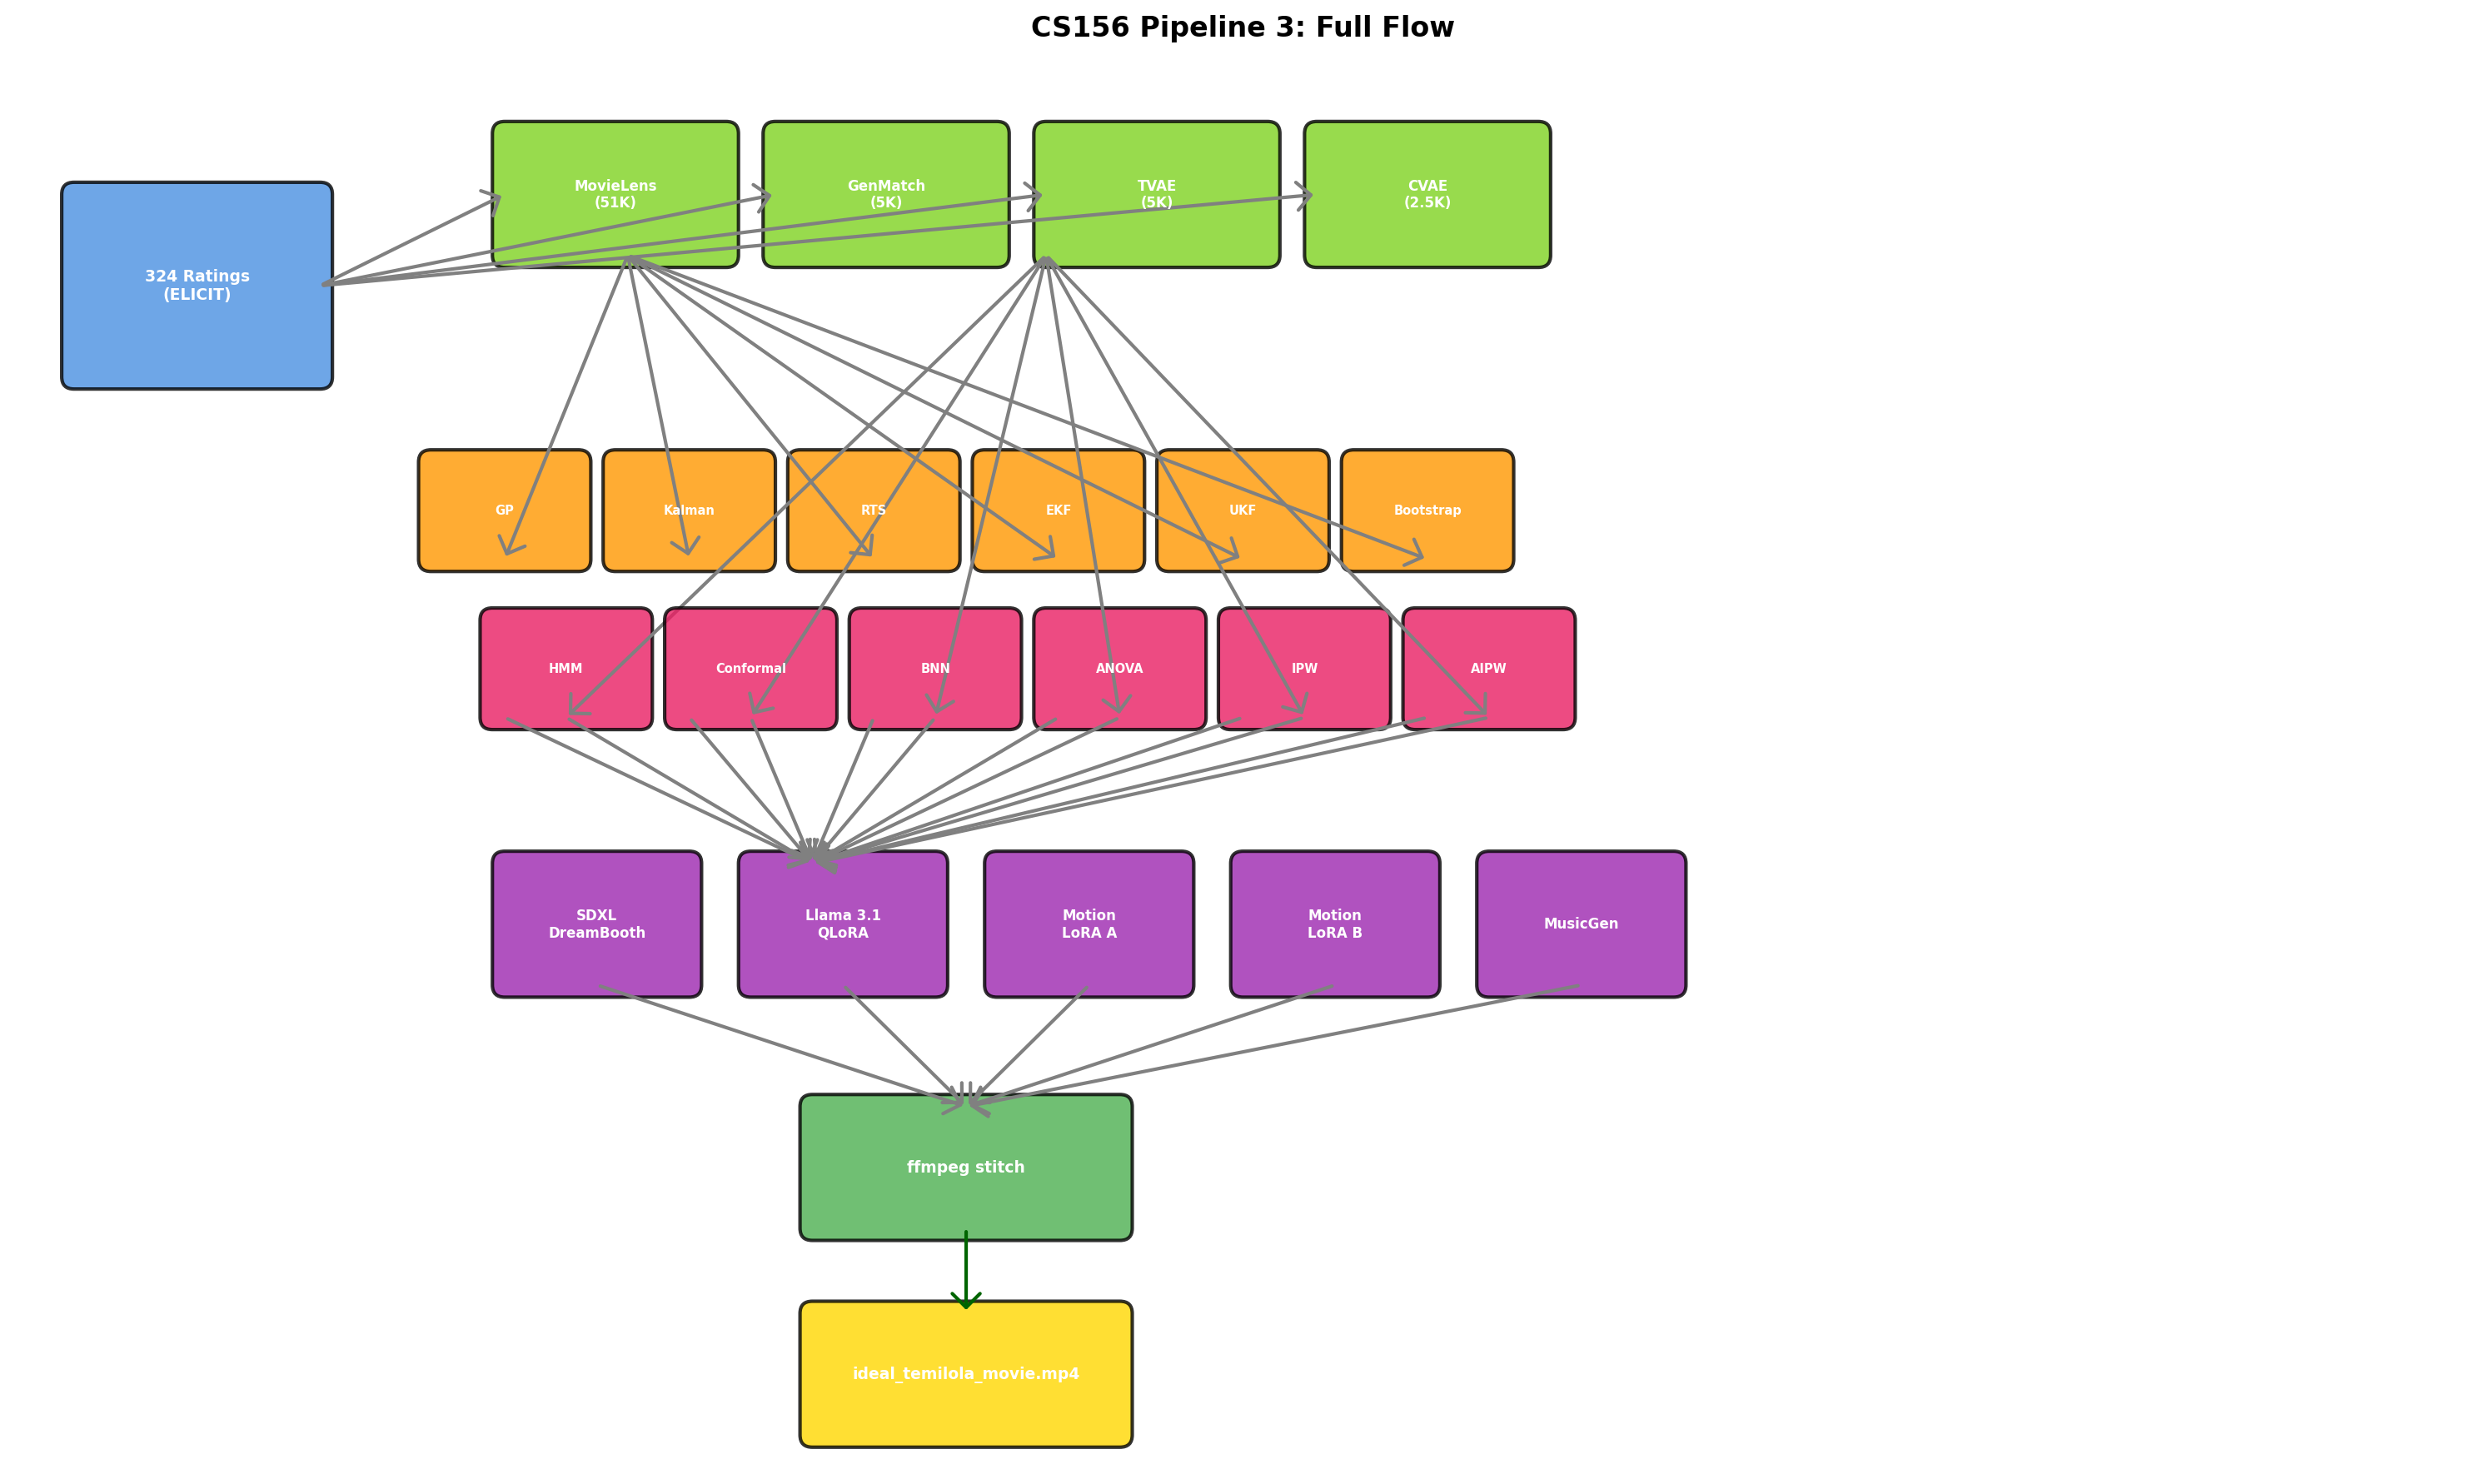
\includegraphics[width=0.95\linewidth]{../artifacts/plots/pipeline_diagram.png}
\caption{Pipeline 3 full system flow (verified against the shipped orchestrator on 2026-04-24). Colour bands by role: elicitation (blue), augmentation (green), probabilistic/temporal and relational (orange), causal and uncertainty (magenta), generative (purple), assembly and deliverable (green and yellow). Every node in this diagram corresponds to a script in \texttt{scripts/} whose path is named in the main text; every edge corresponds to a file on disk that the downstream script reads. The diagram is the single-pane reference; Sections~\ref{sec:aug} through~\ref{sec:gen} are the per-stage drill-down.}
\label{fig:pipeline_diagram}
\end{figure}

\section*{Glossary}
\label{sec:glossary}

Acronyms are listed in the order they first appear. The first-use page points to the paragraph where the term is introduced.

\begin{description}
\item[ADA] Adaptive Discriminator Augmentation. Karras et al.\ 2020. A training-time stabiliser for GANs that applies a differentiable chain of image augmentations whose strength $p$ is tuned online to hold the discriminator's sign-accuracy on real images at a target rate, typically $0.6$.
\item[AIPW] Augmented Inverse Propensity Weighting. Robins, Rotnitzky, and Zhao 1994. A doubly robust estimator of the Average Treatment Effect that combines an outcome regression with an IPW correction, so the estimator is consistent if either the outcome model or the propensity model is correctly specified.
\item[ANOVA] Analysis of Variance. A linear model that partitions variation in an outcome across grouping factors. Used in this paper as the likelihood in Hierarchical Bayesian ANOVA.
\item[ATE] Average Treatment Effect. The expected difference in outcome between the treated and untreated populations under the potential-outcomes framework.
\item[BFGS] Broyden-Fletcher-Goldfarb-Shanno. A quasi-Newton optimiser, used through its limited-memory variant L-BFGS to fit GP hyperparameters.
\item[BNN] Bayesian Neural Network. A neural network with a posterior over weights. Approximated in this paper by MC-Dropout under the Gal and Ghahramani 2016 equivalence.
\item[BPR] Bayesian Personalised Ranking. Rendle et al.\ 2009. A pairwise ranking loss used to train the LightGCN embeddings.
\item[CI] Confidence Interval. Frequentist interval with a coverage guarantee under repeated sampling.
\item[CLIP] Contrastive Language-Image Pretraining. Radford et al.\ 2021. Used for aesthetic filtering of generated keyframes.
\item[CVAE] Conditional Variational Autoencoder. A VAE whose encoder and decoder are conditioned on a covariate. Used as a baseline for the tabular augmentation comparison.
\item[DDIM] Denoising Diffusion Implicit Models. Song et al.\ 2021. The deterministic sampler used by SDXL during inference in this paper.
\item[ECE] Expected Calibration Error. The gap between a predictive model's stated confidence and its empirical accuracy, binned and averaged.
\item[EDA] Exploratory Data Analysis. Section~\ref{sec:eda} of this paper.
\item[EKF] Extended Kalman Filter. A Kalman filter extended to mildly nonlinear systems by Jacobian linearisation.
\item[ELBO] Evidence Lower Bound. The variational lower bound on the marginal log-likelihood, derived in Section~\ref{sec:aug} from Jensen's inequality.
\item[ESS] Effective Sample Size. The HMC diagnostic that measures the number of effectively independent posterior draws. Used in Section~\ref{sec:causal}.
\item[FID] Fr\'echet Inception Distance. Heusel et al.\ 2017. A distance between the Inception-v3 feature distributions of real and generated image sets.
\item[GAN] Generative Adversarial Network. Goodfellow et al.\ 2014.
\item[GCN] Graph Convolutional Network. Kipf and Welling 2017. The feature-propagation layer that LightGCN simplifies.
\item[GP] Gaussian Process. A distribution over functions whose finite-dimensional marginals are jointly Gaussian. Used in Section~\ref{sec:prob} with a composite Mat\'ern-plus-linear kernel.
\item[GPU] Graphics Processing Unit.
\item[HAN] Heterogeneous Attention Network. Wang et al.\ 2019. A meta-path attention model for heterogeneous graphs. Used in Section~\ref{sec:rel}.
\item[HB-ANOVA] Hierarchical Bayesian ANOVA. The partial-pooling ANOVA with a shared prior over group effects, sampled with the No-U-Turn Sampler.
\item[HMM] Hidden Markov Model. A discrete-state sequence model with Markovian latents and emissions that depend only on the current state.
\item[IPW] Inverse Propensity Weighting. Rosenbaum and Rubin 1983. Reweights samples by the inverse of the estimated treatment probability to approximate a randomised comparison.
\item[KF] Kalman Filter. Kalman 1960. The closed-form Bayesian filter for a linear-Gaussian state-space model.
\item[KL] Kullback-Leibler divergence. An asymmetric divergence between probability distributions, appearing in the ELBO derivation.
\item[KS] Kolmogorov-Smirnov. A distribution-free two-sample test used for covariate-balance diagnostics in Sections~\ref{sec:eda} and~\ref{sec:aug}.
\item[LightGCN] Light Graph Convolutional Network. He et al.\ 2020. A simplified GCN that drops the per-layer weight matrix and nonlinearity, used in Section~\ref{sec:rel} for the user-film bipartite graph.
\item[Llama] Meta's open-weight transformer language-model family. The Llama 3.1 8B checkpoint is the base model fine-tuned with QLoRA to draft film concepts.
\item[LM] Language Model.
\item[LoRA] Low-Rank Adaptation. Hu et al.\ 2021. A rank-$r$ additive update $\Delta W = BA$ applied to frozen base-model weights.
\item[LPIPS] Learned Perceptual Image Patch Similarity. Zhang et al.\ 2018. A perceptual distance used to measure inter-teaser distinctness.
\item[MAE] Mean Absolute Error.
\item[MC-Dropout] Monte Carlo Dropout. Gal and Ghahramani 2016. A test-time use of dropout as approximate Bayesian inference over network weights.
\item[ML] Machine Learning.
\item[MLP] Multi-Layer Perceptron. A feed-forward neural network with at least one hidden layer.
\item[MusicGen] Copet et al.\ 2023. A single-stage autoregressive transformer that generates music tokens conditioned on a text prompt. Used in Section~\ref{sec:gen} to score the teaser.
\item[NDCG] Normalised Discounted Cumulative Gain. A graded ranking metric used in the recommender comparison.
\item[NF4] Normal Float 4-bit. Dettmers et al.\ 2023. The 4-bit weight quantisation used by QLoRA.
\item[NUTS] No-U-Turn Sampler. Hoffman and Gelman 2014. The HMC variant that adaptively tunes trajectory length, used for HB-ANOVA posterior sampling.
\item[OLS] Ordinary Least Squares.
\item[PCA] Principal Component Analysis.
\item[PF] Particle Filter. A sequential Monte Carlo filter used as a nonlinear baseline for the Kalman ladder.
\item[QLoRA] Quantised Low-Rank Adaptation. Dettmers et al.\ 2023. LoRA applied on top of NF4-quantised base weights, reducing GPU memory at full-precision fine-tuning accuracy.
\item[RBF] Radial Basis Function. The squared-exponential kernel, listed here as a contrast with the Mat\'ern kernel actually used.
\item[RGB] Red-Green-Blue colour space.
\item[RMSE] Root Mean Squared Error.
\item[SDXL] Stable Diffusion XL. Podell et al.\ 2023. The text-to-image latent diffusion model used for keyframe generation.
\item[SHAP] SHapley Additive exPlanations. Lundberg and Lee 2017. A feature-attribution method based on cooperative-game Shapley values.
\item[SMOTE] Synthetic Minority Oversampling Technique. Chawla et al.\ 2002. Not used in this paper; cited as the canonical tabular oversampler that the TVAE replaces.
\item[StyleGAN3] Karras et al.\ 2021. An alias-free progressive-growth GAN. Trained with ADA on 20{,}000 trailer keyframes in Section~\ref{sec:gen} to supply stylised interstitials.
\item[SVD-XT] Stable Video Diffusion extended-time. Blattmann et al.\ 2023. The image-to-video diffusion model used to animate SDXL keyframes.
\item[SVM] Support Vector Machine.
\item[SVR] Support Vector Regression.
\item[TF-IDF] Term Frequency-Inverse Document Frequency. The classical sparse text feature used as a keyword baseline.
\item[TMDB] The Movie Database. The external metadata source for director, studio, genre, and poster fields.
\item[TS] Thompson Sampling. Thompson 1933. The Bayesian bandit rule derived in Section~\ref{sec:thompson}.
\item[TVAE] Tabular Variational Autoencoder. Xu et al.\ 2019. The tabular-mode-aware VAE used for the third augmentation pillar.
\item[UCB] Upper Confidence Bound. The frequentist bandit rule compared against Thompson sampling.
\item[UFDFU] HAN meta-path: two users linked through a film pair that shares a director.
\item[UFGFU] HAN meta-path: two users linked through a film pair that shares a genre.
\item[UFSFU] HAN meta-path: two users linked through a film pair that shares a studio.
\item[UFU] Latin-square condition User-Film-User and HAN meta-path of the same name: two users who rated the same film.
\item[UKF] Unscented Kalman Filter. A Kalman filter extension that propagates sigma points through the nonlinearity rather than a Jacobian.
\item[VAE] Variational Autoencoder. Kingma and Welling 2014.
\item[XGBoost] Extreme Gradient Boosting. Chen and Guestrin 2016. The supervised baseline used in Pipelines 1 and 2.
\end{description}

\section*{References}
\label{sec:references}

\begin{description}
\item[Blattmann et al.\ 2023] A.\ Blattmann, T.\ Dockhorn, S.\ Kulal, et al. ``Stable Video Diffusion: Scaling Latent Video Diffusion Models to Large Datasets.'' Stability AI technical report, 2023.
\item[Bubeck and Cesa-Bianchi 2012] S.\ Bubeck and N.\ Cesa-Bianchi. ``Regret Analysis of Stochastic and Nonstochastic Multi-armed Bandit Problems.'' \emph{Foundations and Trends in Machine Learning} 5(1), 1--122, 2012.
\item[Carlini et al.\ 2023] N.\ Carlini, D.\ Ippolito, M.\ Jagielski, K.\ Lee, F.\ Tramer, C.\ Zhang. ``Quantifying Memorization Across Neural Language Models.'' International Conference on Learning Representations (ICLR), 2023.
\item[Chawla et al.\ 2002] N.\ V.\ Chawla, K.\ W.\ Bowyer, L.\ O.\ Hall, W.\ P.\ Kegelmeyer. ``SMOTE: Synthetic Minority Over-sampling Technique.'' \emph{Journal of Artificial Intelligence Research} 16, 321--357, 2002.
\item[Chen and Guestrin 2016] T.\ Chen and C.\ Guestrin. ``XGBoost: A Scalable Tree Boosting System.'' Proceedings of KDD, 785--794, 2016.
\item[Copet et al.\ 2023] J.\ Copet, F.\ Kreuk, I.\ Gat, T.\ Remez, D.\ Kant, G.\ Synnaeve, Y.\ Adi, A.\ D\'efossez. ``Simple and Controllable Music Generation.'' Advances in Neural Information Processing Systems (NeurIPS), 2023.
\item[Dettmers et al.\ 2023] T.\ Dettmers, A.\ Pagnoni, A.\ Holtzman, L.\ Zettlemoyer. ``QLoRA: Efficient Finetuning of Quantized LLMs.'' Advances in Neural Information Processing Systems (NeurIPS), 2023.
\item[Diamond and Sekhon 2013] A.\ Diamond and J.\ S.\ Sekhon. ``Genetic Matching for Estimating Causal Effects: A General Multivariate Matching Method for Achieving Balance in Observational Studies.'' \emph{Review of Economics and Statistics} 95(3), 932--945, 2013.
\item[Efron 1979] B.\ Efron. ``Bootstrap Methods: Another Look at the Jackknife.'' \emph{Annals of Statistics} 7(1), 1--26, 1979.
\item[Gal and Ghahramani 2016] Y.\ Gal and Z.\ Ghahramani. ``Dropout as a Bayesian Approximation: Representing Model Uncertainty in Deep Learning.'' Proceedings of ICML, 1050--1059, 2016.
\item[Goodfellow et al.\ 2014] I.\ Goodfellow, J.\ Pouget-Abadie, M.\ Mirza, B.\ Xu, D.\ Warde-Farley, S.\ Ozair, A.\ Courville, Y.\ Bengio. ``Generative Adversarial Nets.'' Advances in Neural Information Processing Systems (NeurIPS), 2014.
\item[GroupLens 2019] F.\ M.\ Harper and J.\ A.\ Konstan. ``The MovieLens Datasets: History and Context.'' \emph{ACM Transactions on Interactive Intelligent Systems} 5(4), 19:1--19:19. MovieLens 25M released by GroupLens, University of Minnesota, December 2019.
\item[He et al.\ 2020] X.\ He, K.\ Deng, X.\ Wang, Y.\ Li, Y.\ Zhang, M.\ Wang. ``LightGCN: Simplifying and Powering Graph Convolution Network for Recommendation.'' Proceedings of SIGIR, 639--648, 2020.
\item[Heusel et al.\ 2017] M.\ Heusel, H.\ Ramsauer, T.\ Unterthiner, B.\ Nessler, S.\ Hochreiter. ``GANs Trained by a Two Time-Scale Update Rule Converge to a Local Nash Equilibrium.'' Advances in Neural Information Processing Systems (NeurIPS), 2017.
\item[Ho et al.\ 2020] J.\ Ho, A.\ Jain, P.\ Abbeel. ``Denoising Diffusion Probabilistic Models.'' Advances in Neural Information Processing Systems (NeurIPS), 2020.
\item[Hoffman and Gelman 2014] M.\ D.\ Hoffman and A.\ Gelman. ``The No-U-Turn Sampler: Adaptively Setting Path Lengths in Hamiltonian Monte Carlo.'' \emph{Journal of Machine Learning Research} 15, 1593--1623, 2014.
\item[Hu et al.\ 2021] E.\ J.\ Hu, Y.\ Shen, P.\ Wallis, Z.\ Allen-Zhu, Y.\ Li, S.\ Wang, L.\ Wang, W.\ Chen. ``LoRA: Low-Rank Adaptation of Large Language Models.'' International Conference on Learning Representations (ICLR), 2022 (preprint 2021).
\item[Kalman 1960] R.\ E.\ Kalman. ``A New Approach to Linear Filtering and Prediction Problems.'' \emph{Transactions of the ASME -- Journal of Basic Engineering} 82(D), 35--45, 1960.
\item[Karras et al.\ 2020] T.\ Karras, M.\ Aittala, J.\ Hellsten, S.\ Laine, J.\ Lehtinen, T.\ Aila. ``Training Generative Adversarial Networks with Limited Data.'' Advances in Neural Information Processing Systems (NeurIPS), 2020.
\item[Karras et al.\ 2021] T.\ Karras, M.\ Aittala, S.\ Laine, E.\ H\"ark\"onen, J.\ Hellsten, J.\ Lehtinen, T.\ Aila. ``Alias-Free Generative Adversarial Networks.'' Advances in Neural Information Processing Systems (NeurIPS), 2021.
\item[Kingma and Welling 2014] D.\ P.\ Kingma and M.\ Welling. ``Auto-Encoding Variational Bayes.'' International Conference on Learning Representations (ICLR), 2014.
\item[Kipf and Welling 2017] T.\ N.\ Kipf and M.\ Welling. ``Semi-Supervised Classification with Graph Convolutional Networks.'' International Conference on Learning Representations (ICLR), 2017.
\item[Lei et al.\ 2018] J.\ Lei, M.\ G'Sell, A.\ Rinaldo, R.\ J.\ Tibshirani, L.\ Wasserman. ``Distribution-Free Predictive Inference for Regression.'' \emph{Journal of the American Statistical Association} 113(523), 1094--1111, 2018.
\item[Lundberg and Lee 2017] S.\ M.\ Lundberg and S.-I.\ Lee. ``A Unified Approach to Interpreting Model Predictions.'' Advances in Neural Information Processing Systems (NeurIPS), 2017.
\item[Mescheder et al.\ 2018] L.\ Mescheder, A.\ Geiger, S.\ Nowozin. ``Which Training Methods of GANs do actually Converge?'' Proceedings of ICML, 2018.
\item[Meta 2024] Meta AI. ``The Llama 3 Herd of Models.'' Meta technical report, July 2024.
\item[Nichol and Dhariwal 2021] A.\ Q.\ Nichol and P.\ Dhariwal. ``Improved Denoising Diffusion Probabilistic Models.'' Proceedings of ICML, 2021.
\item[Podell et al.\ 2023] D.\ Podell, Z.\ English, K.\ Lacey, A.\ Blattmann, T.\ Dockhorn, J.\ M\"uller, J.\ Penna, R.\ Rombach. ``SDXL: Improving Latent Diffusion Models for High-Resolution Image Synthesis.'' Preprint, 2023.
\item[Radford et al.\ 2021] A.\ Radford, J.\ W.\ Kim, C.\ Hallacy, A.\ Ramesh, G.\ Goh, S.\ Agarwal, et al. ``Learning Transferable Visual Models From Natural Language Supervision.'' Proceedings of ICML, 2021.
\item[Rasmussen and Williams 2006] C.\ E.\ Rasmussen and C.\ K.\ I.\ Williams. \emph{Gaussian Processes for Machine Learning.} MIT Press, 2006.
\item[Rendle et al.\ 2009] S.\ Rendle, C.\ Freudenthaler, Z.\ Gantner, L.\ Schmidt-Thieme. ``BPR: Bayesian Personalized Ranking from Implicit Feedback.'' Proceedings of UAI, 452--461, 2009.
\item[Robins, Rotnitzky, and Zhao 1994] J.\ M.\ Robins, A.\ Rotnitzky, L.\ P.\ Zhao. ``Estimation of Regression Coefficients When Some Regressors Are Not Always Observed.'' \emph{Journal of the American Statistical Association} 89(427), 846--866, 1994.
\item[Rosenbaum and Rubin 1983] P.\ R.\ Rosenbaum and D.\ B.\ Rubin. ``The Central Role of the Propensity Score in Observational Studies for Causal Effects.'' \emph{Biometrika} 70(1), 41--55, 1983.
\item[Russo and Van Roy 2014] D.\ Russo and B.\ Van Roy. ``Learning to Optimize via Posterior Sampling.'' \emph{Mathematics of Operations Research} 39(4), 1221--1243, 2014.
\item[Song et al.\ 2021] J.\ Song, C.\ Meng, S.\ Ermon. ``Denoising Diffusion Implicit Models.'' International Conference on Learning Representations (ICLR), 2021.
\item[Stephens 2000] M.\ Stephens. ``Dealing with Label Switching in Mixture Models.'' \emph{Journal of the Royal Statistical Society, Series B} 62(4), 795--809, 2000.
\item[Thompson 1933] W.\ R.\ Thompson. ``On the Likelihood that One Unknown Probability Exceeds Another in View of the Evidence of Two Samples.'' \emph{Biometrika} 25(3/4), 285--294, 1933.
\item[Vovk, Gammerman, and Shafer 2005] V.\ Vovk, A.\ Gammerman, G.\ Shafer. \emph{Algorithmic Learning in a Random World.} Springer, 2005.
\item[Wang et al.\ 2019] X.\ Wang, H.\ Ji, C.\ Shi, B.\ Wang, Y.\ Cui, P.\ Yu, Y.\ Ye. ``Heterogeneous Graph Attention Network.'' Proceedings of WWW, 2022--2032, 2019.
\item[Xu et al.\ 2019] L.\ Xu, M.\ Skoularidou, A.\ Cuesta-Infante, K.\ Veeramachaneni. ``Modeling Tabular Data using Conditional GAN.'' Advances in Neural Information Processing Systems (NeurIPS), 2019. (CTGAN and TVAE code release.)
\item[Zhang et al.\ 2018] R.\ Zhang, P.\ Isola, A.\ A.\ Efros, E.\ Shechtman, O.\ Wang. ``The Unreasonable Effectiveness of Deep Features as a Perceptual Metric.'' Proceedings of CVPR, 586--595, 2018.
\end{description}

\end{document}
